\documentclass[a4paper, 14pt]{extarticle}
\usepackage[margin=1in]{geometry}
\usepackage{amsfonts, amsmath, amssymb, amsthm}
\usepackage[none]{hyphenat}
\usepackage{fancyhdr} %create a custom header and footer
\usepackage[utf8]{inputenc}
\usepackage[english, main=ukrainian]{babel}
\usepackage{pgfplots}
\usepgfplotslibrary{fillbetween}
\usepackage{tikz}
\usepackage{graphicx}
\usepackage{caption}
\usepackage{float}
\usepackage{physics}
\usepackage[unicode]{hyperref}
\usepgfplotslibrary{polar}
\usepackage{ifthen}
\usetikzlibrary{spy}


\fancyhead{}
\fancyfoot{}
\parindent 0ex
\DeclareMathOperator*\uplim{\overline{lim}}
\DeclareMathOperator*\downlim{\underline{lim}}
\def\stackbelow#1#2{\underset{\displaystyle\overset{\displaystyle\shortparallel}{#2}}{#1}}
\def\huge{\displaystyle}
\def\bigline{\vspace{5mm}\\}
\def\rightproof{$\boxed{\Rightarrow}$ }
\def\leftproof{$\boxed{\Leftarrow}$ }

\usepackage{pdfpages}

\newcommand{\sequence}[2][{}]{%
\ifthenelse{\equal{#1}{}}{$\{{#2}, n \geq 1 \}$}
{$\huge \left\{ {#2} = {#1}, n \geq 1 \right\}$}%
}

\newtheoremstyle{theoremdd}% name of the style to be used
  {\topsep}% measure of space to leave above the theorem. E.g.: 3pt
  {\topsep}% measure of space to leave below the theorem. E.g.: 3pt
  {\normalfont}% name of font to use in the body of the theorem
  {0pt}% measure of space to indent
  {\bfseries}% name of head font
  {}% punctuation between head and body
  { }% space after theorem head; " " = normal interword space
  {\thmname{#1}\thmnumber{ #2}\textnormal{\thmnote{ \textbf{#3}\\}}}

\theoremstyle{theoremdd}
\newtheorem{theorem}{Theorem}[subsection]
  
\theoremstyle{theoremdd}
\newtheorem{definition}[theorem]{Definition}

\theoremstyle{theoremdd}
\newtheorem{samedef}[theorem]{Definition}

\theoremstyle{theoremdd}
\newtheorem{example}[theorem]{Example}

\theoremstyle{theoremdd}
\newtheorem{proposition}[theorem]{Proposition}

\theoremstyle{theoremdd}
\newtheorem{remark}[theorem]{Remark}

\theoremstyle{theoremdd}
\newtheorem{lemma}[theorem]{Lemma}

\theoremstyle{theoremdd}
\newtheorem{corollary}[theorem]{Corollary}

\newenvironment{pf}{\vspace*{-3mm} \textbf{Proof. \\}}{$\blacksquare$}
\newenvironment{pfMI}{\vspace*{-3mm} \textbf{Proof MI. \\}}{$\blacksquare$}

%delete
\def\subsequence#1{$\displaystyle \left\{ {#1}, k\geq1 \right\}$}
\def\limitdef#1#2#3#4#5{$\displaystyle \forall #1 > 0: \exists #2(#1): \forall #3 \geq #2: \left|#4 - #5\right| < #1$}
\def\bounded#1#2#3{$\exists #1>0: \forall #2\geq1: \abs{#3} < #1$}

\def\proof{\textbf{Proof.}\\}
\def\qed{$\blacksquare$}

\begin{document}
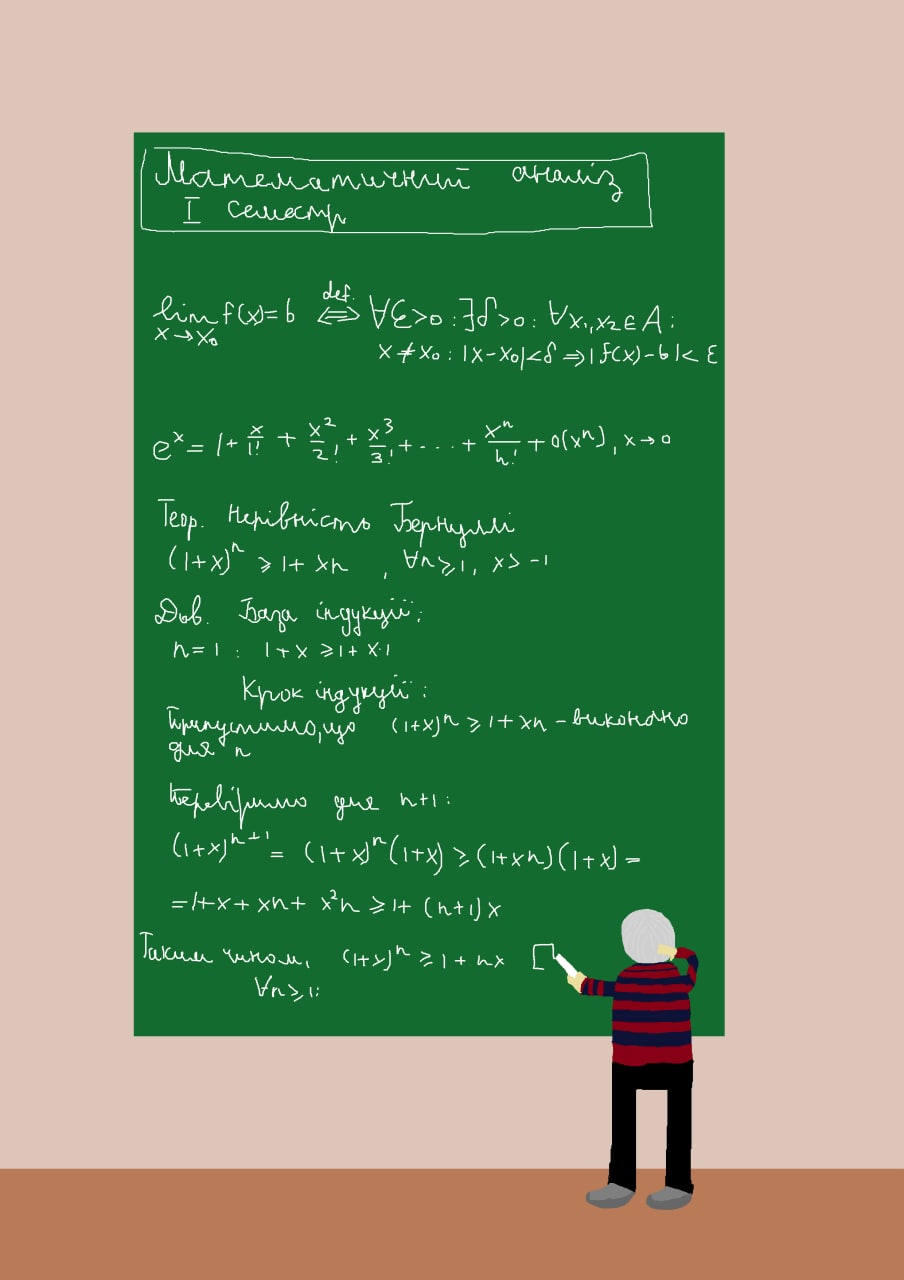
\includepdf{GB.jpg}
\tableofcontents
\newpage

\section*{Початкові нотації}
$\forall$ - для будь-якого, для довільного, ...\\
$\exists$ - існує, знайдеться принаймні один, ...\\
$\exists!$ - існує єдиний\\
$\not \exists$ - не існує
\bigline
$\implies$ - випливає\\
$\iff$ - еквівалентно; тоді й тільки тоді, коли...; 'теж саме, що'
\bigline
$x \in A$ - елемент $x$ належить множині $A$\\
$A \ni x$ - множина $A$ містить елемент $x$
\bigline

\textbf{Авторські нотації:}\\
\textbf{Definition} - означення\\
\textbf{Theorem} - теорема\\
\textbf{Corollary} - наслідок\\
\textbf{Proposition} - твердження\\
\textbf{Lemma} - лема\\
\textbf{Example} - приклад\\
\textbf{Remark} - зауваження\\
\textbf{Proof.} - доведення\\
\textbf{ProofMI.} - доведення методом математичної індукції\\
$\blacksquare$ - кінець доведення\\
! *купа тексту* ! - частина доведення якогось факту від супротивного
\newpage

\section{Комплексні числа}
\subsection{Арифметика}
Комплексним числом будемо називати число такого формату:
\begin{align*}
a + ib
\end{align*}
Тут $a,b \in \mathbb{R}$, тобто будь-яке число\\
А $i$ називають \textbf{уявною одиницею} - таке число, що
\begin{align*}
i^2 = -1
\end{align*}
Множину комплексних чисел ми позначимо за $\mathbb{C}$
\bigline
Якщо у нас є два комплексних числа $a_1 + ib_1$ та $a_2 + ib_2$, а також відомо, що\\
$a_1 + ib_1 = a_2 + ib_2$, то це теж саме, що $\begin{cases} a_1 = a_2 \\ b_1 = b_2 \end{cases}$\\
Більш математично це записується так (використовуючи нотації):\\
$a_1 + ib_1 = a_2 + ib_2 \iff \begin{cases} a_1 = a_2 \\ b_1 = b_2 \end{cases}$\\
\bigline
Основна арифметика: ми можемо два комплексних числа довадати/віднімати, множити та ділити\\
$(a_1+ib_1) \pm (a_2 + ib_2) = (a_1 \pm a_2) + i(b_1 \pm b_2)$
\bigline
$(a_1+ib_1) \cdot (a_2 + ib_2) = a_1 a_2 + a_1 i b_2 + ib_1 a_2 + i^2 b_1 b_2 = (a_1a_2-b_1b_2) + i(a_1b_2+a_2b_1)$
\bigline
З діленням ситуація цікавіша. Спочатку введемо поняття \textbf{комплексно спряжене число} - число формата
\begin{align*}
a - ib
\end{align*}
По суті кажучи, замість знаку $+$ ми ставимо знак $-$\\
Якщо тепер перемножити стандартне комплексне число на його спряжене, то ми отримаємо наступне:
\begin{align*}
(a+ib)(a-ib) = a^2 - (ib)^2 = a^2 + b^2
\end{align*}
Ідея ділення двох комплексних чисел полягає домноженню дроба на комплексно спряжене число знаменника\\
$\dfrac{a_1+ ib_1}{a_2 + ib_2} = \dfrac{(a_1 + ib_1)\textcolor{red}{(a_2-ib_2)}}{(a_2+ib_2)\textcolor{red}{(a_2-ib_2)}} = \dfrac{(a_1a_2 + b_1b_2) + i(a_2b_1-a_1b_2)}{a_2^2 + b_2^2} = \\ = \dfrac{a_1a_2 + b_1b_2}{a_2^2 + b_2^2} + i \dfrac{a_2 b_1 - a_1 b_2}{a_2^2 + b_2^2}$
\bigline
\subsection{Геометрична інтерпретація та додаткова арифметика}
Нехай є комплексне число $z = x + iy, \hspace{0.5cm} x,y \in \mathbb{R}, z \in \mathbb{C}$\\
Нові позначення:\\
$x = \Re z$ - \textbf{дійсна частина} \\
$y = \Im z$ - \textbf{уявна частина}\\
Комплексно спряжене до числа $z$ позначаємо $\bar{z} = x - iy$
\bigline
Копмлексне число можна інтерпретувати як 'вектор' на такій системі координат\\
\begin{tikzpicture}
\draw[thick, ->] (-3,0)--(4,0) node[anchor = north] {$x = \Re z$};
\draw[thick, ->] (0,-2)--(0,4) node[anchor = east] {$y = \Im z$};
\draw[thick, dashed] (-2,2)--(0,2) node[anchor = west] {$y$};
\draw[thick, dashed] (-2,2)--(-2,0) node[anchor = north] {$x$};
\draw[thick, ->, red] (0,0)--(-2,2) node[anchor = south] {$z$};
\draw[black] (0.5,0) arc (0:135:0.5) node at (0.5,0.5) {$\varphi$};
\draw node at (0.2,-0.3) {$0$};
\end{tikzpicture}\\
Можемо знайти \textbf{довжину} комплексного числа - відстань до початку координат\\
$|z| = \sqrt{x^2+y^2}$\\
Із цього випливає наступна формула:\\
$z \cdot \bar{z} (x+iy)(x-iy) = x^2+y^2 = |z|^2$
\bigline
Ще одне нове позначення:\\
$\varphi = \arg z$ - \textbf{аргумент комплексного числа}
\bigline
Повернімось до малюнку та спробуємо знайти $x,y$. За геометрічними міркуваннями:\\
$\begin{cases}
x = |z| \cos \varphi \\
y = |z| \sin \varphi
\end{cases}
$\\
Такі значення $x,y$ ми підставимо в комплексне число $z = x + iy$\\
Отримаємо \textbf{тригонометричну формулу} комплексного числа
\begin{align*}
z = |z|(\cos \varphi + i \sin \varphi)
\end{align*}
З'ясуємо арифметику комплексних чисел в тригонометричній формулі. Нехай є 2 комплексних числа:\\
$z_1 = |z_1| (\cos \varphi_1 + i \sin \varphi_1)$\\
$z_2 = |z_2| (\cos \varphi_2 + i \sin \varphi_2)$
\bigline
1. Множення\\
$z_1 \cdot z_2 = |z_1| |z_2| (\cos \varphi_1 + i \sin \varphi_2) (\cos \varphi_1 + i \sin \varphi_2) = \\ = |z_1| |z_2| (\cos \varphi_1 \cos \varphi_2 - \sin \varphi_1 \sin \varphi_2 + i[\sin \varphi_1 \cos \varphi_2 + \sin \varphi_2 \cos \varphi_1]) = \\
= |z_1||z_2|(\cos (\varphi_1 + \varphi_2) + i \sin(\varphi_1 + \varphi_2))$\\
Отримали, що коли ми множимо два комплексних числа, модулі ми множимо, а аргументи ми додаємо, тобто\\
$\begin{cases}
|z_1 \cdot z_2| = |z_1| \cdot |z_2| \\
\arg(z_1 \cdot z_2) = \arg z_1 + \arg z_2
\end{cases}$\\
$z_1 \cdot z_2 = |z_1||z_2|(\cos (\varphi_1 + \varphi_2) + i \sin(\varphi_1 + \varphi_2))$
\bigline
2. Ділення\\
$\dfrac{z_1}{z_2} \overset{\textrm{позн.}}{=} w$,\\
де $w = |w|(\cos \psi + i \sin \psi)$\\
Ми вже навчилися множити два комплексних числа, тому зведемо таким чином:\\
$z_1 = w z_2 \implies \begin{cases} |z_1| = |z_2| \cdot |w| \\ \arg z_1 = \arg z_2 + \arg w \end{cases} \implies \begin{cases} |z_1| = |z_2| \cdot |w| \\ \varphi_1 = \varphi_2 + \psi \end{cases}$\\
Звідси знайдемо, чому дорівнює $|w|$ та $\psi$\\
$\begin{cases} |w| = \dfrac{|z_1|}{|z_2|} \\ \psi = \varphi_1 - \varphi_2 \end{cases}$\\
В результаті отримаємо:\\
$w = \dfrac{z_1}{z_2} = \dfrac{|z_1|}{|z_2|} (\cos (\varphi_1 - \varphi_2) + i \sin (\varphi_1 - \varphi_2))$
\bigline
3. Зведення в степінь\\
$z^n = z \cdots z = |z| \cdots |z| (\cos(\varphi+\dots+\varphi) + i \sin (\varphi + \dots + \varphi)) = \\ = |z|^n (\cos (n \varphi) + i \sin (n \varphi))$\\
Отримали \textbf{формулу Муавра}
\begin{align*}
z^n = |z|^n (\cos (n \varphi) + i \sin (n \varphi))
\end{align*}
4. Вилучення коренів\\
$\sqrt[n]{z} \overset{\textrm{позн.}}{=} w$,\\
де $w = |w|(\cos \psi + i \sin \psi)$\\
Ми щойно навчилися зводити комплексне число в степінь, тому зведемо таким чином:\\
$z = w^n$\\
$|z|(\cos \varphi + i \sin \varphi) = |w|^n (\cos n \psi + i \sin n \psi)$\\
Отримаємо, що $\begin{cases} |w|^n = z \\ n \psi = \varphi + 2 \pi k \end{cases} \implies \begin{cases} |w| = \sqrt[n]{|z|} \\ \psi = \dfrac{\varphi + 2\pi k}{n} \end{cases}$\\
Більш детальне пояснення другого рівняння системи:\\
Ми мали, що $\cos \varphi = \cos (n \psi)$\\
Оскільки $\cos$ - $2\pi$-періодична функція, то нас влаштовують не лише $\varphi = n \psi$, а також кути $+2\pi$, $+4\pi$, $\dots$\\
В результаті отримаємо:\\
$w = \sqrt[n]{z} = \sqrt[n]{|z|} \left(\cos \dfrac{\varphi + 2\pi k}{n} + i \sin \dfrac{\varphi + 2 \pi k}{n} \right)$\\
$k = 0,1,\dots,n-1$\\
Якщо $k = n$, то ми отримаємо комплексне число для випадку $k = 0$ через періодичність тригонометричних функцій\\
Якщо $k = n+1$, то ми отримаємо комплексне число для випадку $k = 1$ через періодичність тригонометричних функцій\\
$\dots$\\
Якщо $k = -1$, то ми отримаємо комплексне число для випадку $k = n-1$ через періодичність тригонометричних функцій\\
Отже, коли ми витягаємо корінь, ми маємо $n$ штук комплексних чисел
\begin{example}
Знайти $\sqrt[3]{i}$\\
Розпишемо $i = 0 + i \cdot 1$\\
Якщо це намалювати на площині, то отримаємо, що \\ $|i| = \sqrt{0^2+1^2} = 1, \hspace{0.5cm} \arg i = \varphi = \dfrac{\pi}{2}$
\\
\begin{figure}[H]
\centering
\begin{tikzpicture}
\draw[thick, ->] (-2,0)--(3,0) node[anchor = north] {$x = \Re z$};
\draw[thick, ->] (0,-2)--(0,2) node[anchor = east] {$y = \Im z$};
\draw[thick, ->, red] (0,0)--(0,1) node[anchor = south west] {$z = i$};
\draw[black] (0.5,0) arc (0:90:0.5) node at (1.2,0.5) {$\varphi = \dfrac{\pi}{2}$};
\draw node at (0.2,-0.3) {$0$};
\end{tikzpicture}
\end{figure}
А тепер витягаємо корінь:\\
$\sqrt[3]{i} = \sqrt[3]{1} \left( \cos \dfrac{\dfrac{\pi}{2} + 2 \pi k}{3} + i \sin \dfrac{\dfrac{\pi}{2} + 2 \pi k}{3} \right), \hspace{0.5cm} k=0,1,2$\\
$k = 0 \implies \cos \dfrac{\pi}{6} + i \sin \dfrac{\pi}{6} = \dfrac{\sqrt{3}}{2} + \dfrac{1}{2}i$\\
$k = 1 \implies \cos \dfrac{5 \pi}{6} + i \sin \dfrac{5 \pi}{6} = -\dfrac{\sqrt{3}}{2} + \dfrac{1}{2}i$\\
$k = 2 \implies \cos \dfrac{3 \pi}{2} + i \sin \dfrac{3 \pi}{2} = -i$\\
\begin{figure}[H]
\centering
\begin{tikzpicture}
\draw[thick, ->] (-2,0)--(3,0) node[anchor = north] {$x = \Re z$};
\draw[thick, ->] (0,-2)--(0,2) node[anchor = east] {$y = \Im z$};
\draw[thick, ->, red] (0,0)--(0,-1) node[anchor = south west] {$z = -i$};
\draw[thick, ->, red] (0,0)--({sqrt(3)/2},{1/2}) node[anchor = south west] {$z = \dfrac{\sqrt{3}}{2} + \dfrac{1}{2}i$};
\draw[thick, ->, red] (0,0)--({-sqrt(3)/2},{1/2}) node[anchor = south east] {$z = - \dfrac{\sqrt{3}}{2} + \dfrac{1}{2}i$};
\draw node at (0.2,-0.3) {$0$};
\end{tikzpicture}
\end{figure}
\end{example}

\subsection{Квадратні рівняння}
Одна із головних мотивацій створення комплексних чисел - це квадратне рівняння\\
$x^2 = -1$\\
В дійсних числах (в школі) казали, що розв'язків нема. І дійсно, яке б ми число не зводили в квадрат, ми завжди отримуємо додатнє число\\
Тепер ситуація змінюється і ми навчилися вилучати від'ємні корені\\
$x = \sqrt{-1} = \pm i$
\begin{remark}
Там не випадково не написано $\pm$ перед коренем, тому що\\
$\sqrt{z} = \sqrt{|z|} \left( \cos \dfrac{\varphi + 2 \pi k}{n} + i \sin \dfrac{\varphi + 2 \pi k}{n} \right) = \left[ \begin{gathered} \sqrt{|z|} \left(\cos \dfrac{\varphi}{2} + i \sin \dfrac{\varphi}{2} \right) \\ \sqrt{|z|} \left(-\cos \dfrac{\varphi}{2} - i \sin \dfrac{\varphi}{2} \right) \end{gathered} \right. = \\ = \pm \sqrt{|z|} \left(\cos \dfrac{\varphi}{2} + i \sin \dfrac{\varphi}{2} \right)$\\
Тобто вилучаючи квадратний корінь, ми вже отримуємо два значення
\end{remark}
Але тепер можна спокійно розв'язувати квадратні рівняння\\
$az^2 + bz + c = 0$\\
$a \left( z^2 + \dfrac{2b}{2a}z + \left(\dfrac{b}{2a} \right)^2 \right) + c - \dfrac{b^2}{4a} = 0$\\
$a \left(z + \dfrac{b}{2a} \right)^2 = \dfrac{b^2-4ac}{4a}$\\
$\left(z + \dfrac{b}{2a} \right) = \dfrac{b^2-4ac}{a^2}$\\
$z + \dfrac{b}{2a} = \pm \dfrac{\sqrt{b^2-4ac}}{2a}$\\
$z = \dfrac{-b\pm \sqrt{D}}{2a}$\\

\subsection{Показникова формула}
Коли ми множимо два комплексних числа, то аргументи ми додаємо\\
$(\cos \varphi + i \sin \varphi)(\cos \psi + i \sin \psi) = \cos (\varphi + \psi) + i \sin (\varphi + \psi)$\\
Додавання при множенні чогось виявляється в степенях:\\
$a^x a^y = a^{x+y}$\\
Така паралель буде мотивацією нової форми комплексного числа\\
Нехай $z = |z|(\cos \varphi + i \sin \varphi)$\\
\textbf{Показникова форма} має наступний вигляд
\begin{align*}
z = |z|e^{i \varphi}
\end{align*}
Звідси автоматично випливає \textbf{формула Ейлера}
\begin{align*}
e^{i \varphi} = \cos \varphi + i \sin \varphi
\end{align*}
Що таке $e$ і звідки воно, дізнаємось трохи згодом, а поки сприймаємо це так: $e \approx 2.71$
\bigline
Запишемо формулу Ейлера:\\
$e^{i \varphi} = \cos \varphi + i \sin \varphi$ $(1)$\\
Підставимо в цю формулу $-\varphi$, отримаємо:\\
$e^{-i \varphi} = \cos \varphi - i \sin \varphi$ $(2)$\\
$(1) + (2) \implies \cos \varphi = \dfrac{e^{i \varphi} + e^{-i \varphi}}{2}$\\
$(1) - (2) \implies \sin \varphi = \dfrac{e^{i \varphi} - e^{-i \varphi}}{2i}$
\newpage

\section{Інші теми}
\subsection{Гіперболічні функції}
Гіперболічні функції визначимо таким чином:\\
$\sh x = \dfrac{e^x - e^{-x}}{2}$ - \textbf{гіперболічний сінус} \\
$\ch x = \dfrac{e^x + e^{-x}}{2}$ - \textbf{гіперболічний косінус}
\bigline
Коли в стандартній тригонометрії ми мали тотожність\\
$\cos ^2 x + \sin^2 x = 1$\\
то в гіперболічному вигляду воно виглядає так:\\
$\ch ^2 x - \sh ^2 x = 1$\\
Дійсно, $\ch ^2 x - \sh ^2 x = \dfrac{1}{4}(e^{2x} + 2 + e^{-2x} - e^{2x} + 2 - e^{-2x}) = 1$
\bigline
$2 \ch x \sh x = \sh 2x$\\
Дійсно, $2 \dfrac{e^x + e^{-x}}{2} \dfrac{e^x - e^{-x}}{2} = \dfrac{e^{2x}-e^{-2x}}{2} = \sh 2x$
\bigline
\textbf{Геометрична репрезентація}\\
Співвідношення $\cos ^2 x + \sin^2 x = 1$ дає репрезентацію кола $x^2+y^2=1$\\
Співвідношення $\ch ^2 x + \sh^2 x = 1$ водночас дає репрезентацію гіперболи $x^2-y^2=1$
\begin{center}
\begin{tikzpicture}
\draw[thick, ->] (-2,0)--(2,0) node[anchor = north west] {$x$};
\draw[thick, ->] (0,-2)--(0,2) node[anchor = south east] {$y$};
\draw (0,0) circle (1 cm);
\end{tikzpicture}
\qquad
\begin{tikzpicture}
\draw[thick, ->] (-2,0)--(2,0) node [anchor = north west] {$x$};
\draw[thick, ->] (0,-2)--(0,2) node [anchor = south east] {$y$};

\pgfmathsetmacro{\e}{sqrt(2)}   % eccentricity
\pgfmathsetmacro{\a}{1}
\pgfmathsetmacro{\b}{(\a*sqrt((\e)^2-1)}
%\draw (-2pt,-2)--(2pt,-2) node [anchor = north east] {$-b$};
%\draw (-2pt,2)--(2pt,2) node [anchor = south east] {$b$};
\draw plot[domain=-1:1] ({\a*cosh(\x)},{\b*sinh(\x)});
\draw plot[domain=-1:1] ({-\a*cosh(\x)},{\b*sinh(\x)});
\draw[dashed, domain=-1.5:1.5, variable=\x, samples = 1000] plot({\x}, {\b/\a*\x});
\draw[dashed, domain=-1.5:1.5, variable=\x, samples = 1000] plot({\x}, {-\b/\a*\x});
\end{tikzpicture}
\end{center}
\subsection{Полярні координати}
Задано полярний промінь (піввісь)\\
Точка задається такою парою координат: $A(\rho, \varphi)$, де\\
$\varphi$ - кут між промінем, на якій лежить т. $A$, та полярним променем\\
$\rho$ - відстань від початку координат до т. $A$
\begin{center}
\begin{tikzpicture}
\draw[thick, ->] (0,0)--(3,0);
\draw[thick, red] (0,0)--(-1,2) node at (-1,1) {$\rho$};
\draw[fill = black] (-1,2) circle (1pt) node [anchor = south] {$A$};
\draw[black] (0.5,0) arc (0:{180-atan(2)}:0.5) node at (1,0.5) {$\varphi$};
\end{tikzpicture}
\end{center}
Знайдемо зв'язок між полярною та декартовою систем координат\\
\begin{center}
\begin{tikzpicture}
\draw[thick, ->] (0,0)--(3,0);
\draw[thick, red] (0,0)--(-1,2) node at (-0.8,1) {$\rho$};
\draw[fill = black] (-1,2) circle (1pt) node [anchor = south] {$A$};
\draw[black] (0.5,0) arc (0:{180-atan(2)}:0.5) node at (1,0.5) {$\varphi$};
\draw[thick, ->] (-3,0)--(3,0) node[anchor = north west]{$x$};
\draw[thick, ->] (0,-3)--(0,3) node[anchor = south east]{$y$};
\draw[dashed] (-1,2)--(-1,0)  node [anchor = north] {$x_A$};
\draw[dashed] (-1,2)--(0,2)  node [anchor = west] {$y_A$};
\end{tikzpicture}
\end{center}
З геометричних міркувань, отримаємо наступний зв'язок:\\
$\begin{cases}
x_A = \rho \cos \varphi \\
y_A = \rho \sin \varphi
\end{cases}
$
\bigline
Розглянемо тепер рівняння кола\\
$x^2+y^2 = 1$\\
Підставимо щойно отриманий зв'язок. Тоді отримаємо рівняння кола радіуса $R$ із центром в початку координат в полярних системах коордиат\\
$\rho = R$
\\
Рівняння променя, що виходить із початку координат:\\
$\varphi = \varphi_0$, де $\varphi_0$ - якась величина
\begin{center}
\begin{tikzpicture}
\draw[thick, ->] (0,0)--(3,0);
\draw[thick, red, ->] (0,0)--(1,2);
\draw[black] (0.5,0) arc (0:{atan(2)}:0.5) node at (1,0.5) {$\varphi_0$};
\end{tikzpicture}
\end{center}

\begin{example}
Побудуємо $\rho = \sin 3 \varphi$\\
Малювати будемо за точками, але перед цим знайдемо, які кути нас задовільняють\\
$\rho \geq 0 \implies \sin 3 \varphi \geq 0 \implies 3\pi k \leq 3 \varphi \leq \pi + 2 \pi k, k=0,1,2$
\begin{center}
\begin{tabular}{c|c}
$\varphi$ & $\rho$ \\
\hline
$0$ & $0$ \\
$\dfrac{\pi}{18}$ & $\dfrac{1}{2}$ \\
$\dfrac{\pi}{12}$ & $\dfrac{\sqrt{2}}{2}$ \\
$\dfrac{\pi}{9}$ & $\dfrac{\sqrt{3}}{2}$ \\
$\dfrac{\pi}{6}$ & $1$ \\
\end{tabular}
\qquad
\begin{tabular}{c|c}
$\varphi$ & $\rho$ \\
\hline
$\dfrac{2 \pi}{9}$ & $\dfrac{\sqrt{3}}{2}$ \\
$\dfrac{\pi}{4}$ & $\dfrac{\sqrt{2}}{2}$ \\
$\dfrac{5 \pi}{18}$ &  $\dfrac{1}{2}$ \\
$\dfrac{\pi}{3}$ & $0$ \\
\end{tabular} \\
Це ми щойно розглянули більш зручні нам кути з нерівності $3 \pi k \leq 3 \varphi \leq \pi + 2 \pi k$ при $k = 0$
\end{center}

\begin{center}
\begin{tikzpicture}
   \begin{polaraxis}
     \addplot[mark=none,domain=0:360,samples=300] {sin(x*3)};
   \end{polaraxis}
\end{tikzpicture}
\end{center}
Перша пелюстка при $k = 0$, друга пелюстка при $k =1$, третя пелюстка при $k = 2$
\end{example}

\subsection{Про відображення}
\begin{definition}
Задані дві множини $A,B$\\
\textbf{Відображенням} назвемо таке правило $f$, що кожному елементу із множини $A$ відповідає елемент множини $B$\\
Позначення: $f: A \to B$
\end{definition}

\begin{center} {
\begin{tikzpicture}
\fill[red!40] (0,0) ellipse (1cm and 2cm);
\fill[blue!40] (4,0) ellipse (1cm and 2cm);
\node (A1) at (0.7,1) [circle,fill,inner sep=1.5pt]{};
\node (A2) at (-0.5,-0.7) [circle,fill,inner sep=1.5pt]{};
\node (A3) at (0.5,-0.1) [circle,fill,inner sep=1.5pt]{};

\node (B1) at (4+0,1) [circle,fill,inner sep=1.5pt]{};
\node (B2) at (4-0.8,0.2) [circle,fill,inner sep=1.5pt]{};
\node (B3) at (4+0.5,-0.9) [circle,fill,inner sep=1.5pt]{};
\node[anchor = south east] at (0,0) {$A$};
\node[anchor = north west] at (4,0) {$B$};

\draw[thick, ->] (A1)--(B1);
\draw[thick, ->] (A2)--(B3); \draw[thick, ->] (A3)--(B1);
\end{tikzpicture}
}
\end{center}
\begin{definition}
Задані два відображення: $f: A \to B$, $g: B \to C$\\
	\textbf{Композицією відображень} $f$ та $g$ називають відображення \\ $h: A \to B$ таке, що:
	\begin{align*}
	\forall x \in A: h(x) = g(f(x)) \textrm{, або } h(x) = (g \circ f) (x)
	\end{align*}
\end{definition}
	\begin{center} {
\begin{tikzpicture}
\fill[red!40] (0,0) ellipse (1cm and 2cm);
\fill[blue!40] (4,0) ellipse (1cm and 2cm);
\fill[green!40] (8,0) ellipse (1cm and 2cm);

\node[anchor = south east] at (0,1) {$A$};
\node[anchor = south east] at (4,1) {$B$};
\node[anchor = south east] at (8,1) {$C$};

\draw[thick, ->](0.5,0) .. controls (2,1) .. (4,0) node at (2,1.2) {$f$};
\draw[thick, ->](4.5,0) .. controls (6,1) .. (8,0) node at (6,1.2) {$g$};
\draw[thick, ->](0.5,-0.1) .. controls (4,-1) .. (8,-0.1) node at (6,-1) {$h = g \circ f$};;

\end{tikzpicture}
}
\end{center}
\begin{example}
$f,g: \mathbb{R} \to \mathbb{R}$, $f(x) = x^2$, $g(x) = \sin x$\\
	Тоді $h: \mathbb{R} \to \mathbb{R}$, $h(x) = g(f(x)) = \sin x^2$\\
\end{example}

\begin{proposition}
	Задані відображення $f: A \to B$, $g: B \to C$, \\ $h: C \to D$.
	Тоді $h \circ (g \circ f) = (h \circ g) \circ f$
\end{proposition}

\begin{pf}
	$(h \circ (g \circ f)) (x) = h((g \circ f) (x)) = h(g(f(x)))$\\
	$((h \circ g) \circ f) (x) = (h \circ g) (f(x)) = h(g(f(x)))$
\end{pf}

	\begin{figure}[H]
\centering {
\begin{tikzpicture}
\fill[yellow!40] (0,0) ellipse (1cm and 2cm);
\fill[red!40] (4,0) ellipse (1cm and 2cm);
\fill[blue!40] (8,0) ellipse (1cm and 2cm);
\fill[green!40] (12,0) ellipse (1cm and 2cm);

\node[anchor = south east] at (0,1) {$A$};
\node[anchor = south east] at (4,1) {$B$};
\node[anchor = south east] at (8,1) {$C$};
\node[anchor = south east] at (12,1) {$D$};

\draw[thick, ->](0.5,0) .. controls (2,1) .. (4,0) node at (2,1.2) {$f$};
\draw[thick, ->](4.5,0) .. controls (6,1) .. (8,0) node at (6,1.2) {$g$};
\draw[thick, ->](4+4.5,0) .. controls (4+6,1) .. (4+8,0) node at (4+6,1.2) {$h$};
\draw[thick, ->](0.5,-0.1) .. controls (4,-1) .. (8,-0.1) node at (6,0) {$g \circ f$};
\draw[thick, ->](4+0.5,-0.1-1) .. controls (4+4,-1-1) .. (4+8,-0.1-1) node at (4+6,-1-1) {$h \circ g$};
\draw[thick, ->] (0,1.5) .. controls (6,3) .. (12,1.5) node at(6,3.2) {$h \circ (g \circ f) = (h \circ g) \circ f$};
\end{tikzpicture}
}
\end{figure}

\begin{definition}
Задано відображення $f: A \to B$\\
\textbf{Образом} множини $A_0 \subset A$ називається множина
\begin{align*}
f(A_0) = \{f(x) \in B: x \in A_0 \}
\end{align*}
\textbf{Повним прообразом} множини $B_0 \subset B$ називається множина
\begin{align*}
f^{-1}(B_0) = \{x \in A:  f(x) \in B_0 \}
\end{align*}
\end{definition}

\begin{example}
Задано відображення $f: \mathbb{R} \to \mathbb{R}$: $f(x) = x^2$\\
$A = [-5, 4)$\\
$\Rightarrow f(A) = \{f(x) = x^2: x \in [-5, 4) \} = [0, 25]$\\
$\Rightarrow f^{-1}(A) = \{x: f(x) = x^2 \in [-5, 4) \} \overset{x^2 < 4}{=} (-2, 2)$
\end{example}

\begin{proposition}
Справедливі рівності:\\
$1) f^{-1}(A \cup B) = f^{-1}(A) \cup f^{-1}(B)$\\
$2) f^{-1}(A \cap B) = f^{-1}(A) \cap f^{-1}(B)$\\
$3) f^{-1}(\overline{A}) = \overline{f^{-1}(A)}$\\
\textit{Випливає з теорії множин}
\end{proposition}

\begin{remark}
Властивість образів не часто співпадають:\\
$f(A \cap B) \neq f(A) \cap f(B)$
\end{remark}

\subsection{Принцип математичної індукції}
\begin{definition}
Числова множина $E$ називається \textbf{індуктивною}, якщо
\begin{align*}
\forall x \in E: x+1 \in E
\end{align*}
\end{definition}

\begin{example}
Множини $\mathbb{N}$, $\left\{x \in \mathbb{Q}: x > \dfrac{127}{19} \right\}$ - індуктивні
\end{example}
	
	\begin{proposition}
	Множина $\mathbb{N}$ - мінімальна індуктивна множина, що містить одиничку\\
	Інакше кажучи, будь-яка підмножина $E$, що містить одиничку буде надмножиною $\mathbb{N}$, тобто $E \supset \mathbb{N}$
	\end{proposition}
	\begin{pf}
	Зафіксуємо таку індуктивну множину $E$, що $1 \in E$\\
	Покажемо, що $\mathbb{N} \subset E \iff \forall n \in \mathbb{N}: n \in E$\\
	$1 \in E \overset{\textrm{індуктивна}}{\implies} 2 \in E \overset{\textrm{індуктивна}}{\implies} 3 \in E \overset{\textrm{індуктивна}}{\implies} \dots \overset{\textrm{індуктивна}}{\implies} n \in E$\\
	Таким чином, $\mathbb{N} \subset E$
	\end{pf}
	
	\begin{corollary}[Метод математичної індукції]
	Хочемо перевірити, що $\forall n \in \mathbb{N}$ виконується твердження $P(n)$ (може бути якась рівність, нерівність або ще щось)\\
	1. База індукції. Перевірка, що $P(1)$ - виконано\\
	2. Крок індукції. Припускаємо, що $P(n)$ - виконано для $n$ (або для всіх $k \leq n$). На основі цього доводимо, що $P(n+1)$ - виконано\\
	Тоді множина $P = \{n: P(n) - \textrm{виконано}\}$ - індуктивна та містить одиничку\\
	Отже, $\mathbb{N} \subset P$, а це означає, що $\forall n \in \mathbb{N}: P(n)$ - виконано
	\end{corollary}
	
	\begin{example}
	Доведемо рівність: $1 + 2 + \dots + n = \dfrac{n(n+1)}{2}, \forall n \in \mathbb{N}$\\
	Позначимо $P(n) = \left(1 + 2 + \dots + n = \dfrac{n(n+1)}{2} \right)$\\
	1. База індукції. $P(1) = \left(1 = \dfrac{1\cdot 2}{2} = 1 \right)$ - виконано\\
	2. Крок індукції. Припустимо, що $P(n)$ - виконано для фіксованого $n$, тобто\\
	$1 + 2 + \dots + n = \dfrac{n(n+1)}{2}$ $(*)$\\
	Перевіримо, що $P(n+1)$ - виконано\\
	$1 + 2 + \dots + n + (n+1) \overset{(*)}{=} \dfrac{n(n+1)}{2} + (n+1) = \dfrac{n(n+1)+2(n+1)}{2} = \\ = \dfrac{(n+1)(n+2)}{2}$\\
	$\implies P(n+1)$ - виконано\\
	Таким чином, отримали, що $P(n)$ виконано $\forall n \in \mathbb{N}$, або\\
	$1 + 2 + \dots + n = \dfrac{n(n+1)}{2}, \forall n \in \mathbb{N}$\\
	МІ доведено
	\end{example}
	
	\subsection{Біноміальні коефіцієнти, біном Ньютона}
	Зробимо нове позначення: \\ $n\cdot (n-1) \dots 2 \cdot 1 = n!$ - \textbf{факторіал натуралнього числа}\\
	Властивість: $(n+1)! = (n+1) \cdot \underbrace{n \cdot (n-1) \dots 2 \cdot 1}_{n!} = (n+1)n!$\\
	Домовленість: $0! = 1$
	
	\begin{definition}
	\textbf{Біноміальним коефіцієнтом} назвемо ось таке число
	\begin{align*}
	C_n^k = \dfrac{n!}{k!(n-k)!}
	\end{align*}
	Інтерпретація того числа: серед $n$ студентів обрати $k$ студентів, що будуть відраховані
	\end{definition}

	Властивість:\\
	$C_n^k + C_n^{k+1} = C_{n+1}^{k+1}$\\
	\begin{pf}
	\\
	$C_n^k + C_n^{k+1} = \dfrac{n!}{k!(n-k)!} + \dfrac{n!}{(k+1)!(n-(k+1))!} \boxed{=}$\\
	За властивістю факторіала, $(n-k)! = (n-k-1)!(n-k)$, а також $(k+1)! = (k+1)k!$\\
	$\boxed{=} \dfrac{n!}{k!(n-k)(n-k-1)!} + \dfrac{n!}{k!(k+1)(n-k-1)!} = \dfrac{n!}{k!(n-k-1)!} \left(\dfrac{1}{n-k} + \dfrac{1}{k+1} \right) = \\ = \dfrac{n!}{k!(n-k-1)!} \dfrac{n+1}{(n-k)(k+1)} \boxed{=}$\\
	Знову за властивістю факторіала, $(n+1)n! = (n+1)!$, а також \\ $(n-k)(n-k-1)! = (n-k)!$, $(k+1)k! = (k+1)!$ \\
	$\boxed{=} \dfrac{(n+1)!}{(k+1)!(n-k)!} = \dfrac{(n+1)!}{(k+1)!((n+1)-(k+1))!} = C_{n+1}^{k+1}$
	\end{pf}
	\bigline
	\textbf{Трикутник Паскаля}\\
	В школі були такі формули:\\
	$(a+b) = a + b$\\
	$(a+b)^2 = a^2+2ab + b^2$\\
	$(a+b)^3 = a^3 + 3a^2b + 3ab^2 + b^3$\\
	$(a+b)^4 = ?$\\
	Приберімо зараз літери $a,b$ та отримаємо такий малюнок:\\
	\begin{tikzpicture}
	\node at (1,1) {$1$};
	\node at (2,1) {$1$};
	\node at (0.5,0) {$1$};
	\node at (1.5,0) {$2$};
	\draw[->] (0.6,-0.2)--(0.9,-0.8);
	\draw[->] (1.4,-0.2)--(1.1,-0.8);
	\node at (2.5,0) {$1$};
	\node at (0,-1) {$1$};
	\node[red] at (1,-1) {$3$};
	\node at (2,-1) {$3$};
	\node at (3,-1) {$1$};
	\end{tikzpicture}\\
	По краям трикутника ми будемо завжди з одиницями. Червоне число $3$ взялося шляхом додавання двох чисел зверху: $1 + 2$. Якщо дотримуватись аналогічних міркувань, то ми зможемо розширити трикутник Паскаля:\\
	\begin{tikzpicture}
	\node at (1,1) {$1$};
	\node at (2,1) {$1$};
	\node at (0.5,0) {$1$};
	\node at (1.5,0) {$2$};
	\node at (2.5,0) {$1$};
	\node at (0,-1) {$1$};
	\node at (1,-1) {$3$};
	\node at (2,-1) {$3$};
	\node at (3,-1) {$1$};
	
	\node[blue] at (-0.5,-2) {$1$};
	\node[blue] at (0.5,-2) {$4$};
	\node[blue] at (1.5,-2) {$6$};
	\node[blue] at (2.5,-2) {$4$};
	\node[blue] at (3.5,-2) {$1$};
	
	\node at (-1,-3) {$1$};
	\node at (0,-3) {$5$};
	\node at (1,-3) {$10$};
	\node at (2,-3) {$10$};
	\node at (3,-3) {$5$};
	\node at (4,-3) {$1$};
	\node at (1.5,-4) {$\dots$};
	\end{tikzpicture}\\
	Із цього трикутника ми тепер можем знайти $(a+b)^4$, якщо знати, як повернути літери:\\
	$(a+b)^4 = \textcolor{blue}{1} a^4 + \textcolor{blue}{4}a^3 b + \textcolor{blue}{6} a^2  b^2 + \textcolor{blue}{4}a b^3 + \textcolor{blue}{1} b^4$\\
	Формула починається з $a^4$ та $b^0$. А далі степінь $a$ зменшуємо на одиницю, а степінь $b$, навпаки, збільшуємо на одиницю\\
	А тепер узагальнимо це
	\begin{theorem}[Біном Ньютона]
	$(a+b)^n = C_n^0 a^n b^0 + C_n^1 a^{n-1}b + C_n^2 a^{n-2}b^2 + \dots + C_n^{n-1} a b^{n-1} + C_n^n a^0 b^n \overset{\textrm{коротко}}{=} \\ = \huge \sum_{k=0}^n C_n^k a^{n-k} b^k$
	\end{theorem}
	\begin{pfMI}
	1. База індукції. $n = 1 \implies (a+b)^1 = C_1^0 a^1 b^0 + C_1^1 a^0 b^1 = a + b$\\
	2. Крок індукції. Припустимо, що для фіксованого $n$ формула виконана, тобто\\
	$(a+b)^n = \huge \sum_{k=0}^n C_n^k a^{n-k} b^k$\\
	Перевіримо цю формулу для $n+1$\\
	$(a+b)^{n+1} = (a+b)(a+b)^n \overset{\textrm{припущення МІ}}{=} (a+b) \huge \sum_{k=0}^n C_n^k a^{n-k} b^k = \\ = \huge \sum_{k=0}^n C_n^k a^{n-k+1} b^k + \huge \sum_{k=0}^n C_n^k a^{n-k} b^{k+1} = \\ = \textcolor{red}{a^{n+1}} + \huge \sum_{\textcolor{red}{k=1}}^n C_n^k a^{n-k+1} b^k + \huge \sum_{k=0}^{\textcolor{red}{n-1}} C_n^k a^{n-k} b^{k+1} + \textcolor{red}{b^{n+1}} \boxed{=}$\\
	В другій сумі ми замінимо лічильник: $m = k+1$\\
	Було: $0,1,2,\dots, n-1$\\
	Стало: $1,2,3,\dots,n$\\
	$\boxed{=} a^{n+1} + \huge \sum_{k=1}^n C_n^k a^{n-k+1}b^k + \huge \sum_{m=1}^n C_n^{m-1} a^{n-(m-1)}b^{(m-1)+1} + b^{n+1} \boxed{=}$ \\
	Замінимо літеру $m = k$, сума від цього не зміниться\\
	$\boxed{=} a^{n+1} + \huge \sum_{k=1}^n C_n^k a^{n-k+1}b^k + \huge \sum_{k=1}^n C_n^{k-1} a^{n-k+1}b^{k} + b^{n+1} = \\
	= a^{n+1} + \huge \sum_{k=1}^n a^{n-k+1}b^k \left(C_n^k + C_n^{k-1} \right) + b^{n+1} = \\ = a^{n+1} + \huge \sum_{k=1}^n a^{n-k+1}b^k C_{n+1}^k + b^{n+1} = \\
	= C_{n+1}^0 a^{n+1} b^0 + \huge \sum_{k=1}^n a^{n-k+1}b^k C_{n+1}^k + C_{n+1}^{n+1} a^0 b^{n+1} = \sum_{k=0}^{n+1} C_{n+1}^k a^{n-k+1}b^k = \\ = (a+b)^{n+1}$\\
	МІ доведено
	\end{pfMI}
	\newpage
	
	\section{Про множину дійсних чисел}
	\subsection{Аксіоматика}
	Візьмемо якісь числа $a,b,c \in\mathbb{R}$. Тоді наступні твердження/рівності справедливі:\\
	Відносно операції $+$:\\
	$a+b=b+a$ - комутативність\\
	$(a+b)+c=a+(b+c)$ - асоціативність\\
	$\exists 0 \in\mathbb{R}: a+0=a$ - існування нейтрального елементу\\
	$\exists (-a) \in\mathbb{R}: a+(-a)=0$ - існування оберненого елементу\\
	\\
	Відносно операції $\cdot$:\\
	$a \cdot b=b \cdot a$ - комутативність\\
	$(a \cdot b) \cdot c=a \cdot (b \cdot c)$ - асоціативність\\
	$\exists 1 \in\mathbb{R}: a \cdot 1=a$ - існування нейтрального елементу\\
	$\huge \exists \left(\frac{1}{a}\right) \in\mathbb{R}: a \cdot \frac{1}{a}=1$ - існування оберненого елементу\\
	\\
	$(a+b) \cdot c = a \cdot c + b \cdot c$\\
	\\
	Відношення порядка:\\
	Якщо $a>b$, то $a+c>b+c$\\
	Якщо $c>0$ та $a>b$, то $a+c>b$\\
	Якщо $c>0$ та $a>b$, то $a \cdot c>b \cdot c$\\
	\\
	\textbf{Аксіома відокремленості}\\
	Нехай є дві множини $A,B \subset \mathbb{R}$. Відомо, що $\forall a \in A$, $\forall b \in B: a \leq b$. Тоді $\exists c \in \mathbb{R}: a \leq c \leq b$
	\bigline
	\textbf{Remark 3.1.1.} Мотивацією такої аксіоми може слугувати наступний приклад\\
	$A= \{x \in \mathbb{Q}: x^2 < 2\}, B = \{x \in \mathbb{Q}: x^2 > 2\}$\\
	Тут дійсно $\forall a \in A, b \in B: a < b$, але не існує самого числа $c$, що може розділити обидві множини в раціональних числах. Але $c =\sqrt{2} \in \mathbb{R}$, тобто в дійсних числах, все працює. Коротше, цим можна казати, що на числовій прямій тупо всі числа лежать
	\bigline
	\subsection{Точкові межі}
	\begin{definition}
	Задана множина $A \subset \mathbb{R}$\\
	Множина $A$ називається \textbf{обмеженою зверху}, якщо
	\begin{align*}
	\exists c \in \mathbb{R}: \forall a \in A: a \leq c
	\end{align*}
	\end{definition}

	\begin{definition}
	Задана множина $B \subset \mathbb{R}$\\
	Множина $B$ називається \textbf{обмеженою знизу}, якщо
	\begin{align*}
	\exists d \in \mathbb{R}: \forall b \in B: b \geq d
	\end{align*}
	\end{definition}
	
	Множину всіх чисел, що обмежують множину зверху, позначу за $UpperA$, тобто
	\begin{align*}
	UpperA = \{c \in \mathbb{R}: \forall a \in A: a \leq c \}
	\end{align*}
	Множину всіх чисел, що обмежують множину знизу, позначу за $LowerB$, тобто
	\begin{align*}
	LowerB = \{d \in \mathbb{R}: \forall b \in B: b \geq d \}
	\end{align*}
	\begin{example}
	Задана множина $A = \{1-2^{-n} | n \in \mathbb{N}\} = \left\{\dfrac{1}{2}, \dfrac{3}{4}, \dfrac{7}{8}, \dots \right\}$\\
	Є обмеженою зверху, наприклад, числом $2 \in \mathbb{R}$, тобто $\forall a \in A: a < 2$\\
	Є обмеженою знизу, наприклад, числом $0 \in \mathbb{R}$, тобто $\forall a \in A: a > 0$
	\end{example}
	
	\begin{proposition}[\hspace{0.1cm}]
	Якщо $c \in UpperA$ та $c_1 > c$, то $c_1 \in UpperA$\\
	Якщо $d \in LowerB$ та $d_1 < d$, то $d_1 \in LowerB$\\
	\textit{Обидва твердження випливають з визначення множин}
	\end{proposition}
	
	\begin{proposition}
	Множина $UpperA$ обмежена знизу, а множина $LowerB$ обмежена зверху\\
	\textit{Випливає з означень обмеженості}	
	\end{proposition}
	
	\begin{proposition}
	Для множини $UpperA$ існує мінімальний елемент, а для множини $LowerB$ існує максимальний елемент
	\end{proposition}
	\begin{pf}
	$UpperA = \{c \in \mathbb{R}: \forall a \in A: a \leq c \}$\\ За аксіомою відокремленості, $\exists c' \in \mathbb{R}: a \leq c' \leq c \Rightarrow c' \in UpperA$\\
	$\forall c \in UpperA: c' \leq c \Rightarrow c' = \min UpperA$\\
	Для $LowerB$ доведення аналогічне
	\end{pf}
	
	\begin{definition}[\hspace{0.1cm}]
	\textbf{Точковою верхньою межею} називають наступне число:
	\begin{align*}
	\sup A = \min UpperA
	\end{align*}
	\textbf{Точковою нижньою межею} називають наступне число:
	\begin{align*}
	\inf B = \max LowerB
	\end{align*}
	\end{definition}
	
	\begin{theorem}[Критерій супремуму]
	$c' = \sup A \iff \begin{cases} 
	 \forall a \in A: a \leq c' \\
	 \forall \varepsilon > 0: \exists a_{\varepsilon} \in A: a_{\varepsilon} > c' - \varepsilon
	\end{cases}$\\
	Другий пункт каже ось що: якщо ми візьмемо супремум та трохи зменшимо, то ми знайдемо такий елемент, що буде явно більше за 'зменшеного супремуму' - а отже, цей 'зменший супремум' не буде супремумом. І так для кожного зменшеного
	\begin{figure}[H]
	\centering
	\begin{tikzpicture}
	\draw[thick, ->] (0,0)--(5,0) node at (1,0.5) {$A$};
	\draw[thick] (4,-3pt)--(4,3pt) node at (5,0.5) {$c' = \sup A$};
	\draw node at (3.5,0) {$($};
	\draw node at (3.5, -0.5) {$c' - \varepsilon$};
	\draw[thick, red] (3.5,0)--(4,0);
	\end{tikzpicture}
	\caption*{В червоній зоні буде завжди якийсь елемент $a_{\varepsilon}$}
	\end{figure}
	\end{theorem}
	\begin{pf}
	\rightproof Дано: $c' = \sup A$\\
	Тоді автоматично $c' \in UpperA$, тобто $\forall a \in A: a \leq c'$\\
	Оскільки це мінімальне значення, то\\ $\forall \varepsilon > 0: c' - \varepsilon \notin UpperA \Rightarrow \exists a_{\varepsilon} \in A: a_{\varepsilon} > c' - \varepsilon$
	\bigline
	\leftproof Дано: система з двох умов\\
	Із першої умови випливає, що  $c' \in UpperA$, а із другої умови - \\$c' = \min UpperA = \sup A$
	\end{pf}
	\begin{theorem}[Критерій інфімуму]
	$d' = \inf B \iff \begin{cases} 
	 \forall b \in B: b \geq d'\\
	 \forall \varepsilon > 0: \exists b_{\varepsilon} \in B: b_{\varepsilon} < d' + \varepsilon
	\end{cases}$\\
	\textit{Доведення є аналогічним до критерію супремуму}
	\end{theorem}

	\begin{example} 
	Повернімось до множини \\ $A = \{1-2^{-n} | n \in \mathbb{N}\} = \left\{\dfrac{1}{2}, \dfrac{3}{4}, \dfrac{7}{8}, \dots \right\}$\\
	Доведемо, що $\sup A = 1$\\
	Дійсно, $\forall a \in A: a = 1 - \dfrac{1}{2^n} < 1$\\
	Залишилось довести, що $\forall \varepsilon > 0: \exists a_{\varepsilon}: a_{\varepsilon} > 1 - \varepsilon$\\
	Або $\exists n: 1 - 2^{-n} > 1 -\varepsilon \Rightarrow n > - \log_2 \varepsilon$
	\end{example}
	\begin{definition}
	Множина $F \subset \mathbb{R}$ називається \textbf{обмеженою}, якщо
	\begin{align*}
	\exists p>0: \forall f \in F: |f| \leq p
	\end{align*}
	\end{definition}
	
	\begin{remark}[\hspace{0.1cm}]
	Якщо $A$ не є обмеженою зверху, то вважаємо $\sup A = +\infty$\\
	Якщо $B$ не є обмеженою знизу, то вважаємо $\inf B = -\infty$
	\end{remark}
	
	\subsection{Основні нерівності}
	\begin{theorem}[Нерівність Бернуллі]
	Для всіх $x>-1$ виконується нерівність:
	\begin{align*}
	(1+x)^n \geq 1+nx
	\end{align*}
	\end{theorem}
	\begin{pfMI}
	1. База індукції. $n=1$: $(1+x)^1 \geq 1+1\cdot x$. Нерівність виконується\\
	2. Крок індукції. Нехай для фіксованого $n$ дана нерівність виконується. Доведемо для значення $n+1$\\
	$(1+x)^{n+1}=(1+x)\textcolor{red}{(1+x)^n} \textcolor{red}{\geq} (1+x)\textcolor{red}{(1+nx)}=1+(n+1)x+nx^2 \geq \\ \overset{\textrm{оскільки } x^2 \geq 0}{\geq} 1+(n+1)x$\\
	Отже, така нерівність справедлива $\forall n \geq 1$\\
	МІ доведено
	\end{pfMI}
	\\
	\begin{theorem}[Нерівність Коші]
	Для всіх $a_1, \cdots, a_n \geq 0$ виконується нерівність:
	\begin{align*}
	\frac{a_1+\cdots+a_n}{n} \geq \sqrt[n]{a_1 \cdots a_n}
	\end{align*}
	\end{theorem}
	\begin{pf}
	Тимчасове перепозначення: $\huge A_n = \frac{a_1+\cdots+a_n}{n}$, $\huge G_n = \sqrt[n]{a_1 \cdots a_n}$\\
	Зрозуміло, що $\huge \frac{A_n}{A_{n-1}} > 0 \Rightarrow \frac{A_n}{A_{n-1}}-1>-1$. Тоді за нерівністю Бернуллі\\
	$\huge \left(1+ \left(\frac{A_n}{A_{n-1}} -1 \right) \right)^n \geq 1 + n \cdot \left(\frac{A_n}{A_{n-1}} -1 \right)$\\
	$\Rightarrow \huge \frac{(A_n)^n}{(A_{n-1})^n} \geq \frac{a_n}{A_{n-1}}$\\
	$\Rightarrow \huge (A_n)^n \geq a_n (A_{n-1})^{n-1}$, $\forall n \geq 1$. Тоді\\
	$(A_n)^n \geq a_n (A_{n-1})^{n-1} \geq \cdots \geq a_n a_{n-1} \cdots a_1$. Отже,\\
	$A_n \geq G_n$, що й хотіли довести
	\end{pf}
	\\
	\begin{theorem}[Нерівність трикутника]
	Для довільних $x,y \in \mathbb{R}$ справедлива нерівність:
	\begin{align*}
	|x+y|\leq|x|+|y|
	\end{align*}
	\end{theorem}
	\begin{pf}
	$(|x+y|)^2=(x+y)^2=x^2+2xy+y^2 = |x|^2 + 2xy + |y|^2 \leq |x|^2 + 2|x||y|+|y|^2 = \\ = (|x|+|y|)^2$\\
	$\Rightarrow |x+y| \leq |x|+|y|$
	\end{pf}
	\\
	
	\subsection{Аксіома Архімеда та основні наслідки}
	\textbf{Аксіома Архімеда}\\
	Множина натуральних чисел $\mathbb{N}$ не є обмеженою зверху, тобто
	\begin{align*}
	\forall a \in \mathbb{R}: \exists n \in \mathbb{N}: n > a
	\end{align*}
	
	\begin{corollary}
	Множина цілих чисел $\mathbb{Z}$ не є обмеженою взагалі
	\end{corollary}
	\begin{pf}
	Відомо, що $\forall a \in \mathbb{R}: \exists n \in \mathbb{N}: n > a$\\
	Тоді $\exists m \in \mathbb{N}: (-a) < m \iff (-m) < a$\\
	А число $-m \in \mathbb{Z}$
	\end{pf}
	
	\begin{corollary}
	Задано таке число $a$, що\\
	- $a \geq 0$ \\
	- $\forall \varepsilon > 0: a < \varepsilon$\\
	Тоді $a = 0$
	\end{corollary}
	
	\begin{pf}
	!Припустимо, що $a \neq 0$, тобто лишається випадок $a > 0$\\
	Тоді звідси $\dfrac{1}{a} > 0$\\
	За аксіомою Архімеда, $\exists n \in \mathbb{N}: n > \dfrac{1}{a} \iff a > \dfrac{1}{n}$\\
	Проте нам відомо, що $\forall \varepsilon > 0: a < \varepsilon$. Суперечність!\\
	Таким чином, $a = 0$
	\end{pf}
	
	\begin{corollary}
	Задані такі два числа $a, \in \mathbb{R}$, що $a < b$\\
	Тоді $\exists q = \dfrac{m}{n} \in \mathbb{Q} | m \in \mathbb{Z}, n \in \mathbb{N}: a < \dfrac{m}{n} < b$\\
	Інакше кажучи, в будь-якому інтервалі $(a,b)$ знайдеться принаймні одне раціональне число
	\end{corollary}
	
	\begin{pf}
	$a < b$, тоді розглянемо число $b-a>0 \overset{\textrm{аксіома Архімеда}}{\implies} \exists n: \dfrac{1}{n} < b-a$\\
	Розглянемо таке число $m$, що $\dfrac{m-1}{n} \leq a$ та $\dfrac{m}{n} > a$\\
	!Припустимо, що $\dfrac{m}{n} \geq b$, ми цим кажемо, що $\dfrac{m}{n}$ НЕ потрапляє в інтервал $(a,b)$\\
	Тоді маємо: $b - a \leq \dfrac{m}{n} - \dfrac{m-1}{n} = \dfrac{1}{n}$\\
	Отримали, що $b-a \leq \dfrac{1}{n}$ - суперечність! Оскільки в нас була нерівність навпаки\\
	Таким чином, $\dfrac{m}{n} < b$\\
	Остаточно: $a < \dfrac{m}{n} < b \implies q = \dfrac{m}{n} \in (a,b)$
	\end{pf}
	
	\begin{corollary}
	Задано число $h > 0$ - одиниця шкали, масштаб\\
	Тоді $\forall x \in \mathbb{R}: \exists ! m \in \mathbb{Z}: (m-1)h \leq x \leq mh$
	\end{corollary}
	
	\begin{pf}
	Маємо $h>0$. Із аксіоми Архімеда випливає, що\\
	$\exists !m \in \mathbb{Z}: \dfrac{x}{h} < m$, а також $m-1 \leq \dfrac{x}{h}$\\
	Отже, $m-1 \leq \dfrac{x}{h} \leq m \implies (m-1)h < x \leq mh$
	\end{pf}
	
	\begin{remark}
	Якщо встановити $n = 1$, то $\exists !m \in \mathbb{Z}: m-1 \leq x < m$\\
	В такому випадку позначимо $m-1 = [x]$ - \textbf{ціла частина} числа $x$\\
	Тобто найближче менше ціле число\\
	$[2.6] = 2, [-1.1] = -2$
	\end{remark}
	
	\subsection{Основні твердження мат. аналізу}
	\begin{lemma}[Лема Кантора про вкладені відрізки]
	Задані відрізки наступним чином: $\forall n \geq 1: [a_n, b_n] \supset [a_{n+1}, b_{n+1}]$. Інакше кажучи, $[a_1, b_1] \supset [a_2, b_2] \supset \dots$ Тоді\\
	1) $\exists c \in \mathbb{R}: \forall n \geq 1: c \in [a_n,b_n]$\\
	2) Якщо $\forall \varepsilon > 0: \exists n \in \mathbb{N}: b_n - a_n < \varepsilon$, то $\exists! c \in \mathbb{R}: \forall n \geq 1: c \in [a_n,b_n]$
	\end{lemma}
	\begin{figure}[H]
	\centering
	\begin{tikzpicture}
	\draw[thick, ->] (0,0)--(6,0);
	\draw node at (0.5,0) {$[$}; \draw node at (5.5,0) {$]$};
	\draw node at (1.5,0) {$[$}; \draw node at (4.5,0) {$]$};
	\draw node at (2,0.5) {$\dots$}; \draw node at (4,0.5) {$\dots$};
	\draw node at (2.5,0) {$[$}; \draw node at (3.5,0) {$]$};
	
	\draw node at (0.5,-0.5) {$a_1$}; \draw node at (5.5,-0.5) {$b_1$};
	\draw node at (1.5,-0.5) {$a_2$}; \draw node at (4.5,-0.5) {$b_2$};
	\draw node at (2.5,-0.5) {$a_n$}; \draw node at (3.5,-0.5) {$b_n$};
	\end{tikzpicture}
	\end{figure}
	\begin{pf}
	1) Із умови випливає, що $\forall n,m \in \mathbb{N}:$\\
	$a_1 \leq a_2 \leq \dots \leq a_n \leq \dots < \dots \leq b_n \leq \dots \leq b_2 \leq b_1$\\
	Отже, $\forall n,m \in \mathbb{N}: a_n \leq b_m$\\
	Тому що:\\
	- $n < m: a_n \leq \dots \leq a_m < b_m \leq \dots \leq b_n$\\
	- $n > m: a_n < b_n \leq \dots \leq b_m$\\
	Розглянемо множини $A = \{a_1,\dots,a_n\}, B = \{b_1, \dots, b_m\}$\\
	$\forall a_n \in A: \forall b_m \in B: a_n \leq b_m$\\
	Тоді за аксіомою відокремленості, $\exists c \in \mathbb{R}: \forall n,m \in \mathbb{N}: a_n \leq c \leq b_m$\\
	Таким чином, $\forall n \geq 1: c \in [a_n,b_n]$
	\bigline
	2) Розглянемо окремо, коли $\forall \varepsilon > 0: \exists n: b_n - a_n < \varepsilon$\\
	!Припустимо, що $\exists c' \in \mathbb{R}:$, тобто ще один елемент, що $\forall n \geq 1: \\ c' \in [a_n,b_n]$, але $c \neq c'$\\
	Задамо $\varepsilon = |c' - c| > 0$\\
	Тоді $\exists n: b_n - a_n < \varepsilon$, але $c,c' \in [a_n,b_n]$ для заданого $n$\\
	Тому $\varepsilon = |c'-c| < a_n-b_n < \varepsilon$ - суперечність!\\
	Отже, така точка $c$ є єдиною, причому\\
	$[a_1, b_1] \cap [a_2, b_2] \cap \dots = \{c\}$
	\end{pf}
	
	\begin{definition}
	Задано множина $A \subset \mathbb{R}$\\
	Точка $a_0 \in \mathbb{R}$ називатимемо \textbf{граничною точкою} множини $A$, якщо
	\begin{align*}
	\forall \varepsilon > 0: (a_0 - \varepsilon, a_0 + \varepsilon) \cap A \textrm{ - нескінченна множина}
	\end{align*}
	Водночас інтервал $(a_0 - \varepsilon, a_0 + \varepsilon) \overset{\textrm{позн.}}{=} U_{\varepsilon}(a_0)$ називають \textbf{$\varepsilon$-окілом} т. $a_0$
	\end{definition}
	
	\begin{example}
	Задано множина $A = [0,1)$. Знайдемо всі граничні точки\\
	1. $a \in (0,1)$\\
	$\forall \varepsilon > 0: (a-\varepsilon,a+\varepsilon) \cap [0,1) = \left[ \begin{gathered} \left[0, a + \varepsilon \right) \textrm{або } (0,1), \varepsilon \geq a \\ \left(a-\varepsilon,a+\varepsilon \right) \textrm{або} \left(a, 1\right), 0 < \varepsilon < a \end{gathered} \right.$\\
	Всі множини є нескінченними\\
Отже: із $(0,1)$ всі точки є граничними
\bigline
	2.1) $a = 0$\\
	$(a-\varepsilon, a+\varepsilon) \cap [0,1) = [0,a+\varepsilon)$ або $[0,1)$ - нескінченні множини. Тож $a = 0$ - гранична\\
	2.2) $a = 1$\\
	$(a-\varepsilon, a+\varepsilon) \cap [0,1) = (1-\varepsilon,1)$ або $[0,1)$ - нескінченні множини. Тож $a = 1$ - гранична
	\bigline
	3.1) $a < 0$\\
	Розглянемо $\varepsilon = \dfrac{-a}{2}$\\
	Тоді $(a-\varepsilon,a+\varepsilon) = \left(\dfrac{3a}{2}, \dfrac{a}{2} \right) \subset \left(\dfrac{3a}{2},0 \right)$\\
	$\implies (a-\varepsilon,a+\varepsilon) \cap [0,1) = \emptyset$ - порожня множина\\
	Отже, жодна точка, яка $a < 0$, не є граничною
	\bigline
	3.2) $a > 1$\\
	Розглянемо $\varepsilon = \dfrac{a-1}{2}$\\
	Тоді $(a-\varepsilon,a+\varepsilon) = \left(\dfrac{a+1}{2}, \dfrac{3a-1}{2} \right) \subset \left(1, \dfrac{3a-1}{2} \right)$\\
	$\implies (a-\varepsilon,a+\varepsilon) \cap [0,1) = \emptyset$ - порожня множина\\
	Отже, жодна точка, яка $a > 1$, не є граничною
	\end{example}
	
	\begin{example}
	Задано множина $A = \left\{\dfrac{1}{n} | n \in \mathbb{N} \right\} = \left\{1, \dfrac{1}{2}, \dfrac{1}{3}, \dots \right\}$. Знайдемо всі граничні точки\\
	1. $a \in (0,1]$\\
	Ми завжди можемо знайти номер $n \in \mathbb{N}$, що $\dfrac{1}{n+1} \leq a \leq \dfrac{1}{n}$\\
	Зафіксуємо $\varepsilon = \dfrac{1}{(n+1)^{20}}$. Тоді $(a-\varepsilon,a+\varepsilon) \cap A = \emptyset$ або $= \dfrac{1}{n}$
	\bigline
	2. $a > 1$\\
	Зафіксуємо $\varepsilon = \dfrac{a-1}{2}$. Тоді $(a-\varepsilon,a+\varepsilon) \cap A = \emptyset$
	\bigline
	3. $a < 0$\\
	Зафіксуємо $\varepsilon = \dfrac{-a}{2}$. Тоді $(a-\varepsilon,a+\varepsilon) \cap A = \emptyset$
	\bigline
	4. $a = 0$\\
	Тоді $\forall \varepsilon > 0: (a-\varepsilon,a+\varepsilon) \cap A = (-\varepsilon, + \varepsilon) \cap A$ - нескінчення множина\\
	Тому що $\exists N: \forall n \geq N:$ $\dfrac{1}{n} < \varepsilon \iff n > \dfrac{1}{\varepsilon}$\\
	Остаточно: $a = 0$ - єдина гранична точка
	\end{example}
	
	\begin{theorem}[Теорема Больцано-Вейєрштрасса]
	Задано множина $A$ - обмежена множина з нескінченною кількістю елементів. Тоді вона містить принаймні одну граничну точку
	\end{theorem}
	
	\begin{pf}
	Оскільки $A$ - обмежена, то:\\
	$\exists a \in \mathbb{R}: \forall x \in A: x \geq a$\\
	$\exists b \in \mathbb{R}: \forall x \in A: x \leq b$\\
	Тобто маємо множину $A \subset [a,b]$\\
	Розіб'ємо множину $[a,b]$ навпіл: $\left[a, \dfrac{a+b}{2}\right]$ та $\left[\dfrac{a+b}{2},b \right]$\\
	Оскільки $A$ має нескінченну кількість чисел, то принаймні одна з множин $\left[a, \dfrac{a+b}{2}\right] \cap A$ або $\left[\dfrac{a+b}{2}, b\right] \cap A$ - нескінченна множина. Ту половину позначимо за множину $[a_1,b_1]$ (якщо обидва нескінченні, то вибір довільний). Тоді $A \cap [a_1,b_1]$ - нескінченна множина\\
	Розіб'ємо множину $[a_1,b_1]$ навпіл: $\left[a_1, \dfrac{a_1+b_1}{2}\right]$ та $\left[\dfrac{a_1+b_1}{2},b_1 \right]$\\
	І за аналогічними міркуваннями одна з множин нескінченна, позначу за $[a_2,b_2]$. Тоді $A \cap [a_2,b_2]$ - нескінченна множина\\
	Розіб'ємо множину $[a_2,b_2]$ навпіл: $\left[a_2, \dfrac{a_2+b_2}{2}\right]$ та $\left[\dfrac{a_2+b_2}{2},b_2 \right]$\\
	$\dots$\\
	В результаті матимемо вкладені відрізки: $[a,b] \supset [a_1,b_1] \supset [a_2,b_2] \supset \dots$\\
	Причому $\forall n: b_n - a_n = \dfrac{b-a}{2^n}$\\
	Зафіксуємо $\varepsilon > 0$ та перевіримо, чи існує $n$, що $b_n - a_n < \varepsilon$\\
	Маємо: $\dfrac{b-a}{2^n} < \varepsilon \Rightarrow \dots \Rightarrow n > \log_2 \dfrac{b-a}{\varepsilon}$\\
	Тоді за лемою Кантора, $\exists! c \in \mathbb{R}: \forall n \geq 1: c \in [a_n,b_n]$\\
	А далі покажемо, що $c$ - дійсно гранична точка множини $A$\\
	Зафіксуємо $\varepsilon > 0$. Знайдемо, чи існує $n$: $b_n - a_n = \dfrac{b-a}{2^n} < \dfrac{\varepsilon}{2} \Rightarrow \dots \Rightarrow n > \log_2 \dfrac{2(b-a)}{\varepsilon}$\\
	Тоді $[a_n,b_n] \subset (c-\varepsilon, c+\varepsilon)$, оскільки $c-a_n \leq \dfrac{\varepsilon}{2}$ та $b_n -c \leq \dfrac{\varepsilon}{2}$\\
	І це все виконується $\forall \varepsilon > 0$\\
	Таким чином, $A \cap (c-\varepsilon, c+\varepsilon) \supset A \cap [a_n,b_n]$ - нескінченна множина, а отже, $c$ - гранична точка $A$
	\end{pf}
	\newpage
	
	\section{Границі числової послідовності}
	\subsection{Основні означення}
	\begin{definition}
	\textbf{Числовою послідовністю} називають якийсь набір чисел \sequence{a_n}\\
	Тобто кожному номеру $n$ буде зіставлено якесь число $a_n$
	\end{definition}

	\begin{definition}
	Число $a$ називається \textbf{границею числової послідовності} \sequence{a_n}, якщо справедливе таке твердження:
	\begin{align*}
	\forall \varepsilon > 0: \exists N(\varepsilon) \in \mathbb{N}: \forall n \geq N: |a_n - a| < \varepsilon
	\end{align*}
	Позначення: $\displaystyle \lim_{n \to \infty} a_n = a$ або $a_n \overset{n \to \infty}{\longrightarrow} a$\\
	Якщо в деякої послідовності існує чисельна границя, то така послідовність називається \textbf{збіжною}. В інакшому випадку - \textbf{розбіжна}
	\end{definition}
	
	\begin{theorem}
	Для збіжної границі існує єдина границя
	\end{theorem}
	
	\begin{pf}
	!Припустимо, задана збіжна числова послідовність \sequence{a_n}, для якої існують дві границі:\\
	$\displaystyle \lim_{n \to \infty} a_n = a, \lim_{n \to \infty} a_n = b$\\
	Врахуємо, що $a<b$ (для $a>b$ міркування є аналогічними)\\
	Оскільки границі існують, ми можемо задати $\displaystyle \varepsilon = \frac{b-a}{3}$. Тоді\\
	$\displaystyle \exists N_1: \forall n \geq N_1: |a_n-a|< \frac{b-a}{3} \Rightarrow a_n < a + \frac{b-a}{3}$\\
	$\displaystyle \exists N_2: \forall n \geq N_2: |a_n-b|< \frac{b-a}{3} \Rightarrow a_n > b - \frac{b-a}{3}$\\
	Аби обидві нерівності працювали одночасно, ми зафіксуємо новий \\ $N= \max\{N_1,N_2\}$. Тоді:\\
	$\displaystyle \forall n \geq N: a_n < \frac{a+(a+b)}{3} < \frac{b+(a+b)}{3}<a_n$\\
	Отримали суперечність! Отже, обидва ліміти не існують одночасно
	\end{pf}
	
	\begin{example}
	Доведемо за означенням, що $\displaystyle\lim_{n \to \infty} \frac{1}{n} = 0$\\
	Задане довільне $\varepsilon > 0$. Необхідно знайти $\displaystyle N: \forall n \geq N: \left|\frac{1}{n}-0 \right|<\varepsilon$\\
	$\huge \abs{\frac{1}{n} - 0} < \varepsilon \iff \displaystyle \frac{1}{n}<\varepsilon \iff n > \frac{1}{\varepsilon}$\\
	Зафіксуємо $\displaystyle N = \left[\frac{1}{\varepsilon} \right] + 1$. Тоді маємо:\\
	$\forall \varepsilon > 0: \exists N = \huge \left[\frac{1}{\varepsilon} \right] + 1: \forall n \geq N: n > \frac{1}{\varepsilon} \Rightarrow \abs{\frac{1}{n} - 0} < \varepsilon$\\
	Отже, означення виконується, тому $\displaystyle\lim_{n \to \infty} \frac{1}{n} = 0$\\
	\begin{figure}[H]
\centering
\resizebox{0.8\textwidth}{!} {
\begin{tikzpicture}
\draw[thick, ->] (-1,0)--(15cm,0) node[anchor = north] {$n$};
\draw[thick, ->] (0,-1)--(0,8.5cm) node[anchor = east] {$a_n$};
\foreach \x in {1,2,4,8,11}
	\draw (\x cm, 1pt) -- (\x cm, -1pt) node[anchor = north] {$\x$};
	
\foreach \i [evaluate=\i as \x using 8/ \i] in {1,2,4,8}
	\draw (1pt, \x cm) -- (-1pt, \x cm) node[anchor = east] {$\frac{1}{\i}$};


\foreach \x in {1,2,...,15}
	\node[blue] at (\x,8/\x) [circle,fill,inner sep=1.5pt]{};
	
	\draw[thick, red, dashed] (-1,0.1*8)--(15,0.1*8) node[anchor = south] {$0+\varepsilon$};
	\draw[thick, red, dashed] (-1,-0.1*8)--(15,-0.1*8) node[anchor = north] {$0-\varepsilon$};
\end{tikzpicture}
}
\caption*{Як працює означення границі на малюнку. Тут на малюнку я обрав $\varepsilon = 0.1$. Тоді починаючи з $n=11$ (або з $12$, $13$,...), всі решта члени не покидатимуть червоного коридору.
Якщо члени не будуть покидати ці лінії для будь-якого заданого $\varepsilon$, то тоді границя існує}
\end{figure}
\end{example}

\begin{example}
Доведемо за означенням, що $\displaystyle\lim_{n \to \infty} \sqrt[n]{n}=1$\\
	Знову задамо довільне $\varepsilon > 0$. Знову необхідно знайти $\displaystyle N: \forall n \geq N: \left|\sqrt[n]{n}-1  \right|<\varepsilon \iff \sqrt[n]{n}<1+\varepsilon$\\
	Використовуючи нерівність Коші, ми отримаємо таку оцінку:\\
	$\displaystyle \sqrt[n]{n}= \sqrt[n]{\sqrt{n}\cdot\sqrt{n}\cdot 1 \cdots 1} \leq \frac{\sqrt{n}+\sqrt{n}+1+\cdots+1}{n} = \frac{2\sqrt{n}+n-2}{n} = \\ = \frac{2}{\sqrt{n}}+1-\frac{2}{n}<\frac{2}{\sqrt{n}}+1$. Тоді:\\
	$\displaystyle \sqrt[n]{n} < \frac{2}{\sqrt{n}} + 1 < 1 + \varepsilon \iff \frac{2}{\sqrt{n}} < \varepsilon \iff n > \frac{4}{\varepsilon^2}$\\
	Тепер зафіксуємо $\displaystyle N = \left[\frac{4}{\varepsilon^2} \right] + 2021$. Ну й тоді $\forall n \geq N$ всі нерівності виконуються, зокрема $\left|\sqrt[n]{n}-1  \right|<\varepsilon$\\
	Остаточно, $\displaystyle\lim_{n \to \infty} \sqrt[n]{n}=1$
\end{example}

\begin{example}
	Доведемо за означенням, що $\displaystyle\lim_{n \to \infty} \frac{n^k}{b^n} = 0$, $b>1$\\
	Вже було доведено в {\textbf{Ex. 4.1.5.}}, що $\displaystyle\lim_{n \to \infty} \sqrt[n]{n}=1$, а тому означення працює:
	\limitdef{\varepsilon'}{N_0}{n}{\sqrt[n]{n}}{1} $\iff \sqrt[n]{n}<1+\varepsilon'$\\
	Оскільки границя існує, ми оберемо $\displaystyle \varepsilon' = \sqrt[2k]{b}-1$. Тоді:\\
	$\displaystyle \sqrt[n]{n} < 1 + \sqrt[2k]{b}-1 \iff n^k < b^{\frac{n}{2}}$\\
	Отже, ми отримали, що $\forall n \geq N_0: n^k < b^{\frac{n}{2}}$. Дану оцінку використаємо для доведення бажаного ліміту\\
	\\
	Зафіксуємо інше $\varepsilon>0$. Хочемо знайти $N_1: \forall n \geq N_1: \displaystyle \abs{\frac{1}{b^{\frac{n}{2}}}} < \varepsilon$\\
	$\displaystyle \iff \cdots \iff n>2 \log_{b} \frac{1}{\varepsilon}$. Тоді $\displaystyle N_1 = \left[\log_{b} \frac{1}{\varepsilon} \right] + 2^2$\\
	Нарешті, якщо зафіксувати $N=\max\{N_0, N_1\}$, то $\forall n \geq N$ справедлива оцінка:\\
	$\displaystyle \abs{\frac{n^k}{b^n}} < \abs{\frac{1}{b^{\frac{n}{2}}}} < \varepsilon'$\\
	\\
	Остаточно, $\forall \varepsilon > 0: \exists N = \max\{N_0(\varepsilon), N_1(\varepsilon)\}: \forall n \geq N: \abs{\dfrac{n^k}{b^k} - 0} < \varepsilon$\\
	$\overset{\textrm{def.}}{\iff} \displaystyle\lim_{n \to \infty} \frac{n^k}{b^n} = 0$, $b>1$
\end{example}

\begin{example}
	Доведемо, що не існує $\displaystyle \lim_{n \to \infty} (-1)^n$\\
	Припускаємо, що даний ліміт збіжний, тобто $\displaystyle \lim_{n \to \infty} (-1)^n = a$, тобто\\
	\limitdef{\varepsilon}{N}{n}{(-1)^n}{a}. Тоді\\
	$\displaystyle 2=\abs{(-1)^n-(-1)^{n+1}}=\abs{((-1)^n)-a+(a-(-1)^{n+1})} \overset{\textrm{нер-ть трикутника}}{\leq} \\ \leq \abs{(-1)^n-a}+\abs{a-(-1^{n+1})} < 2\varepsilon \Rightarrow \varepsilon > 1$\\
	Прийшли до суперечності. Тому даний ліміт існувати не може\\
	\begin{figure}[H]
\centering
\resizebox{0.7\textwidth}{!} {
\begin{tikzpicture}
\draw[thick, ->] (-1,0)--(8.5,0) node[anchor = north] {$n$};
\draw[thick, ->] (0,-1.5)--(0,1.7) node[anchor = east] {$a_n$};
\foreach \x in {1,2,...,8}
	\draw (\x cm, 1pt) -- (\x cm, -1pt) node[anchor = north] {$\x$};
	
\draw (1pt, 1 cm) -- (-1pt,1 cm) node[anchor = east] {$1$};
\draw (1pt, -1 cm) -- (-1pt,-1 cm) node[anchor = east] {$-1$};
\foreach \i [evaluate=\i as \x using (-1)^(\i)] in {1,2,...,8}
	\node[blue] at (\i,\x) [circle,fill,inner sep=1.5pt]{};
	
	\draw[thick, red, dashed] (-1,1+0.5)--(8.5,1+0.5) node[anchor = south west] {$1+\varepsilon$};
	\draw[thick, red, dashed] (-1,1-0.5)--(8.5,1-0.5) node[anchor = north west] {$1-\varepsilon$};
	\draw[thick, gray] (-1,1)--(8.5, 1) node[anchor = south] {$a$};
\end{tikzpicture}
}
\caption*{Тут на малюнку я встановил границю $a=1$. Лише для деяких $\varepsilon$ всі члени потраплятимуть всередину. Однак, скажімо, не для $\varepsilon = 0.5$ як на малюнку, ось чому ліміт не може бути рівним $1$. І так для кожного $a$}
\end{figure}
\end{example}

\begin{definition}
	Послідовність \sequence{a_n} називається \textbf{обмеженою}, якщо \begin{align*}
	\exists C>0: \forall n \geq 1: |a_n|\leq C
	\end{align*}
\end{definition}

\begin{theorem}
	Будь-яка збіжна послідовність є обмеженою
\end{theorem}

\begin{pf}
	Нехай задана збіжна послідовність \sequence{a_n}, тобто для неї\\ $\displaystyle \exists \lim_{n \to \infty} a_n = a \overset{\textrm{def.}}{\iff}$ \limitdef{\varepsilon}{N}{n}{a_n}{a}\\
	Оскільки ліміт існує, то задамо $\varepsilon = 1$. Тоді: $\forall n \geq N: \abs{a_n-a}<1$
	Спробуємо оцінити вираз $|a_n|$ для нашого бажаного:\\
	$|a_n| = |a_n - a + a| \leq |a_n-a|+|a| < 1 + |a|$. Це виконується $\forall n \geq N$. Інакше кажучи, всі числа, починаючи з $N$, є обмеженими.\\
	Покладемо $C=\max\{|a_1|,|a_2|,\cdots, |a_{N-1}|, 1+|a|\}$. Тоді отримаємо, що\\
	$\forall n\geq1: |a_n|\leq C$, що й позначає обмеженість
\end{pf}

\begin{remark}
Обернене твердеження не є вірним\\
В {\textbf{Ex. 4.1.7.}} послідовність \sequence[(-1)^n]{a_n} є обмеженою, але не збіжна
\end{remark}

\begin{definition}
	Посідовність \sequence{a_n} \textbf{має границю} $\infty$ (тобто або $+\infty$, або $-\infty$), якщо виконується твердження: 
	\begin{align*}
	\forall E>0: \exists N(E) \in \mathbb{N}: \forall n \geq N: |a_n|>E
	\end{align*}
	Якщо $+\infty$, то $a_n > E$\\
	Якщо $-\infty$, то $-a_n > E$
\end{definition}

\begin{example}
	Доведемо за означенням, що $\displaystyle\lim_{n \to \infty} 2^n = +\infty$\\
	Задано довільне $E>0$. Необхідно знайти $N: \forall n \geq N: 2^n>E \iff n>\log_2{E}$\\
	Фіксуємо $N=\left[\log_2{E} \right] + 2^2$. Тоді $\forall n \geq N$ виконується остання нерівність, а отже, початкова\\
	Тому $\displaystyle\lim_{n \to \infty} 2^n = +\infty$\\
	\begin{figure}[H]
\centering
\resizebox{0.6\textwidth}{!} {
\begin{tikzpicture}
\draw[thick, ->] (-1cm,0)--(5.5cm,0) node[anchor = north] {$n$};
\draw[thick, ->] (0,-1cm)--(0,4.5cm) node[anchor = east] {$a_n$};
\foreach \x in {1,2,...,4}
	\draw (\x cm, 1pt) -- (\x cm, -1pt) node[anchor = north] {$\x$};
	
\foreach \i [evaluate=\i as \x using 2^(\i)/4] in {1,2,...,4}
	\node[blue] at (\i,\x) [circle,fill,inner sep=1.5pt]{};
\foreach \i [evaluate=\i as \x using 2^(\i)/4] [evaluate=\i as \y using int(2^\i)] in {1,2,...,4}
	\draw (1pt, \x) -- (-1pt,\x) node[anchor = east] {$\y$};
	\draw[thick, red, dashed] (-1cm,1.5)--(5.5cm,1.5) node[anchor = south west] {$E$};
	%\draw[thick, red, dashed] (-1,1-0.5)--(8.5,1-0.5) node[anchor = north west] {$1-\varepsilon$};
	%\draw[thick, gray] (-1,1)--(8.5, 1) node[anchor = south] {$a$};
\end{tikzpicture}
}
\caption*{Тут на малюнку $E = 6$. Тоді починаючи з $n=3$ (або з $4$, $5$,...), всі решта члени будуть вище за червону лінію. Тому границя є - це плюс нескінченність}
\end{figure}
\end{example}
	
	\subsection{Нескінченно малі/великі послідовності}
	\begin{definition}[\hspace{0.1cm}]
	Якщо послідовність \sequence{a_n} містить границю $\displaystyle\lim_{n \to \infty} a_n = 0$, то така послідовність називається \textbf{нескінченно малою (н.м.)}\\
	Якщо послідовність \sequence{a_n} містить границю $\displaystyle\lim_{n \to \infty} a_n = \infty$, то така послідовність називається \textbf{нескінченно великою (н.в.)}
	\end{definition}
	
	\begin{example}
	Зокрема \sequence[\dfrac{1}{n}]{a_n} є нескінченно малою, а \sequence[2^n]{b_n} є нескінченно великою, виходячи з минулих прикладів
	\end{example}
	
	\begin{theorem}[Арифметика н.м. та н.в.]
	Задані такі послідовності:\\
	1. \sequence{a_n} - н.м.;\\
	2. \sequence{b_n} - н.м.;\\
	3. \sequence{c_n} - обмежена;\\
	4. \sequence{d_n} - н.в.;\\
	5. \sequence{p_n} - послідовність, що віддалена від 0 \\ ($\exists \delta>0: \forall n\geq 1: |p_n|\geq \delta$)\\
	Тоді наступні послідовності:\\
	1) \sequence{a_n+b_n} - н.м.\\
	2) \sequence{C \cdot a_n} - н.м.\\
	3) \sequence{c_n \cdot a_n} - н.м.\\
	4) \sequence{\dfrac{1}{a_n}} - н.в.\\
	5) \sequence{\dfrac{1}{d_n}} - н.м.\\
	6) \sequence{p_n \cdot d_n} - н.в.
	\end{theorem}
	
	\begin{pf}
	1) $\displaystyle \lim_{n \to \infty} a_n = 0, \lim_{n \to \infty} b_n = 0 \overset{\textrm{def.}}{\iff}$\\
	\limitdef{\varepsilon}{N_1}{n}{a_n}{0} $\displaystyle \Rightarrow |a_n|<\frac{\varepsilon}{2}$\\
	\limitdef{\varepsilon}{N_2}{n}{b_n}{0} $\displaystyle \Rightarrow |b_n|<\frac{\varepsilon}{2}$\\
	Нехай існує $N=\max\{N_1,N_2\}$. Тоді $\forall n \geq N:$\\
	$|a_n+b_n| \leq |a_n|+|b_n| < \varepsilon$\\
	Отже, \sequence{a_n+b_n} - н.м.
	\bigline
	3) $\displaystyle \lim_{n \to \infty} a_n = 0 \overset{\textrm{def.}}{\iff}$ \limitdef{\varepsilon}{N}{n}{a_n}{0} $\Rightarrow \displaystyle |a_n| < \frac{\varepsilon}{M}$\\ 
	Також \bounded{M}{n}{c_n}\\
	Тоді $\forall n \geq N: |a_n \cdot c_n| = |a_n| \cdot |c_n| < \varepsilon$\\
	Отже, \sequence{a_n \cdot c_n} - н.м.
	\bigline
	4) $\displaystyle \lim_{n \to \infty} a_n = 0 \overset{\textrm{def.}}{\iff}$ \limitdef{\varepsilon}{N}{n}{a_n}{0} $\Rightarrow \displaystyle |a_n| < \varepsilon$\\
	Зафіксуємо $\displaystyle \varepsilon = \frac{1}{E}$. Тоді $\displaystyle \forall n \geq N: |a_n|<\frac{1}{E} \iff \abs{\frac{1}{a_n}} > E$\\
	Отже, \sequence{\dfrac{1}{a_n}} - н.в.\\
	2), 6) доводиться як 3). 5) доводиться аналогічно як 4)
	\end{pf}
	
	\begin{remark}
	Є випадки, які НЕ дають точний результат:\\
	1) н.в + н.в.\\
	2) н.м. $\cdot$ н.в.\\
	3) $\dfrac{\textrm{н.м.}}{\textrm{н.м.}}$, $\dfrac{\textrm{н.в.}}{\textrm{н.в.}}$
	\end{remark}
	
	\begin{lemma}[Про характеризацію збіжної послідовності]
	Послідовність \sequence{a_n} є збіжною $\iff a_n=a+\alpha_n$, \\ де \sequence{\alpha_n} - н.м.
	\end{lemma}
	\begin{pf}
	\boxed{\Rightarrow} Дано: \sequence{a_n} - збіжна, тобто\\
	\limitdef{\varepsilon}{N}{n}{a_n}{a}\\
	Позначимо $a_n-a=\alpha_n$. Тоді $a_n=a+\alpha_n$ та послідовність \sequence{\alpha_n} - н.м., оскільки $|\alpha_n - 0| = |\alpha_n| = |a_n - a| < \varepsilon$
	\bigline
	\boxed{\Leftarrow} Дано: \sequence{\alpha_n} - н.м., де $a_n = a + \alpha_n$. Тоді\\
	\limitdef{\varepsilon}{N}{n}{\alpha_n}{0} $\Rightarrow |a_n-a|<\varepsilon$\\
	Отже, \sequence{a_n} - збіжна
	\end{pf}
	
	\begin{theorem}
	Задані \sequence{a_n}, \sequence{b_n} та \\ $\exists \huge \lim_{n \to \infty} a_n = a, \exists \huge \lim_{n \to \infty} b_n = b$ Тоді:\\
	1) $\displaystyle \exists \lim_{n \to \infty} (a_n+b_n) = \lim_{n \to \infty} a_n+\lim_{n \to \infty} b_n$\\
	2) $\displaystyle \forall C \in \mathbb{R}: \exists \lim_{n \to \infty} C \cdot a_n = C \lim_{n \to \infty} a_n$\\
	3) $\displaystyle \exists \lim_{n \to \infty} (a_n \cdot b_n) = \lim_{n \to \infty} a_n \cdot \lim_{n \to \infty} b_n$\\
	4) $\displaystyle \exists \lim_{n \to \infty} \frac{a_n}{b_n} = \frac{\displaystyle \lim_{n \to \infty} a_n}{\displaystyle \lim_{n \to \infty} b_n}_{\neq 0}$
	\end{theorem}
	\begin{pf}
	Обидва послідовності збіжні $\iff$ $a_n = a + \alpha_n$, \sequence{\alpha_n} - н.м., а також $b_n=b+\beta_n$, \sequence{\beta_n} - н.м.\\
	Тоді:\\
	1) $a_n+b_n=a+\alpha_n+b+\beta_n=(a+b)+(\alpha_n+\beta_n)$, причому \sequence{\alpha_n + \beta_n} - н.м. $\iff$ послідовність \sequence{a_n+b_n} має границю:\\ $\displaystyle \lim_{n \to \infty} (a_n+b_n) = a+b = \lim_{n \to \infty} a_n+\lim_{n \to \infty} b_n$\\ \\
	2) довести самостійно\\ \\
	3) $a_n b_n - ab = (a+\alpha_n)(b+\beta_n) - ab = \alpha_n b + \alpha_n \beta_n + a \beta_n = \gamma_n$, причому послідовність \sequence{\gamma_n} - н.м. $\iff$ послідовність \sequence{a_n b_n} має границю:\\
	$\displaystyle \lim_{n \to \infty} (a_n \cdot b_n) = ab = \lim_{n \to \infty} a_n \cdot \lim_{n \to \infty} b_n$\\ \\
4) В принципі, це є наслідком 3), якщо представити послідовність \\ $\dfrac{a_n}{b_n} = a_n \cdot \dfrac{1}{b_n}$\\
	Треба лишень довести, що $\dfrac{1}{b_n} \to \dfrac{1}{b}, n \to \infty$\\
	Відомо, що $b_n \to b \iff \forall \varepsilon > 0: \exists N': \forall n \geq N: |b_n-b| < \varepsilon$\\
	Зафіксую $\varepsilon = \dfrac{|b|}{2}$, тоді $\exists N: \forall b \geq N'': \forall n \geq N'': \\ |b_n| = |b_n - b + b| \leq |b_n - b| + |b| < \dfrac{3|b|}{2}$\\
	Я хочу одночасно $|b_n| < \dfrac{3|b|}{2}$ та $|b_n - b| < \varepsilon$, тож нехай $N = \max \{N', N'' \}$, тоді\\
	$\forall n \geq N: \abs{\dfrac{1}{b_n} - \dfrac{1}{b}} = \dfrac{|b_n -b|}{|b_n| |b|} < \dfrac{\varepsilon}{ \dfrac{3|b|}{2} |b|} = \dfrac{2}{3} \varepsilon$\\
	Таким чином, можна твердити, що $\dfrac{1}{b_n} \to \dfrac{1}{b}, n \to \infty$
	\end{pf}
	
	\begin{example}
	Знайти границю $\displaystyle\lim_{n \to \infty} \frac{2n^2-3n+5}{1-n-3n^2}$\\
	$\displaystyle\lim_{n \to \infty} \frac{2n^2-3n+5}{1-n-3n^2} =\lim_{n \to \infty} \frac{\displaystyle 2-\frac{3}{n}+\frac{5}{n^2}}{\displaystyle \frac{1}{n^2}-\frac{1}{n}-3} = \frac{\displaystyle \lim_{n \to \infty} 2-\frac{3}{n}+\frac{5}{n^2}}{\displaystyle \lim_{n \to \infty} \frac{1}{n^2}-\frac{1}{n}-3} =\\ = \frac{\displaystyle \lim_{n \to \infty} 2- \lim_{n \to \infty} \frac{3}{n}+ \lim_{n \to \infty} \frac{5}{n^2}}{\displaystyle \lim_{n \to \infty} \frac{1}{n^2}- \lim_{n \to \infty}\frac{1}{n}- \lim_{n \to \infty} 3} = \frac{2-0+5}{0-0-3} = -\frac{2}{3}$
	\end{example}
	
	\begin{remark}
	Більш детально, чому рівності спрацьовують:\\
	Оскільки існують ліміти в четвертому дробі, то існують ліміти в третьому дробі (як сума), то тоді існує ліміт в другому дробі (як частка)
	\end{remark}
	
	
	\subsection{Нерівності в границях}	
	\begin{theorem}
	Задані дві збіжні числові послідовності \sequence{a_n}, \sequence{b_n} таким чином, що $\exists N': \forall n \geq N': a_n \leq b_n$. Тоді\\ $\displaystyle \lim_{n \to \infty} a_n \leq \lim_{n \to \infty} b_n$
	\end{theorem}
	
	\begin{pf}
	Задані дві збіжні послідовності, для яких $\displaystyle \lim_{n \to \infty} a_n =a, \lim_{n \to \infty} b_n = b$\\
	Припустимо, що $a>b$ та розглянемо $\displaystyle \varepsilon = \frac{a-b}{2}$. Тоді за означенням границі,\\
	$\exists N_1: \forall n \geq N_1:|a_n-a|<\varepsilon \Rightarrow a_n>a-\varepsilon$\\
	$\exists N_2: \forall n \geq N_2:|b_n-b|<\varepsilon \Rightarrow b_n<b+\varepsilon$\\
	Задамо $N=\max \{N_1, N_2\}$. Тоді\\ $\displaystyle b_n < b+\varepsilon = b + \frac{a-b}{2}=\frac{a+b}{2}=a-\frac{a-b}{2} = a-\varepsilon<a_n \Rightarrow b_n<a_n$. Суперечність!
	\end{pf}
	
	\begin{corollary}
	Задана збіжна числова послідовность \sequence{b_n} таким чином, що $\exists N': \forall n \geq N': a \leq b_n$. Тоді $\displaystyle a \leq \lim_{n \to \infty} b_n$\\
	\textit{Вказівка: розглянути послідовність \sequence{a_n=a} - так звана стаціонарна послідовність}
	\end{corollary}
	
	\begin{remark}
	Для інших нерівностей: $<$, $\geq$, $>$ - ці теореми теж працюють 
	\end{remark}
	
	\begin{theorem}[Теорема про 3 послідовності]
	Задані три послідовності: \sequence{a_n},\sequence{b_n},\sequence{c_n} таким чином, що $\displaystyle \lim_{n \to \infty} a_n = \displaystyle \lim_{n \to \infty} b_n = a$. Більш того, $\exists N': \forall n \geq N': a_n \leq c_n \leq b_n$.\\
	Тоді $\exists \displaystyle \lim_{n \to \infty} c_n = a$\\
	Така теорема має іншу назву: "про двох поліцаїв"
	\end{theorem}

	\begin{pf}
	$\displaystyle \lim_{n \to \infty} a_n = a \overset{\textrm{def.}}{\iff}$ \limitdef{\varepsilon}{N_1}{n}{a_n}{a} $\Rightarrow a_n > a - \varepsilon$\\
	$\displaystyle \lim_{n \to \infty} b_n = a \overset{\textrm{def.}}{\iff}$ \limitdef{\varepsilon}{N_2}{n}{b_n}{a} $\Rightarrow b_n<a+\varepsilon$\\
	Зафіксуємо $N=\max\{N_1, N_2, N'\}$. Тоді $\forall n \geq N:$\\
	$a-\varepsilon< a_n \leq c_n \leq b_n < a+\varepsilon \Rightarrow |c_n - a|<\varepsilon$\\
	Отже, $\displaystyle \lim_{n \to \infty} c_n = a$
	\end{pf}
	
	\begin{example}
	Знайти границю $\displaystyle \lim_{n \to \infty} \sqrt[n]{2^n+7^n}$\\
	Можна отримати наступну оцінку:\\
	$\sqrt[n]{7^n} \leq \sqrt[n]{2^n+7^n} \leq \sqrt[n]{n\cdot 7^n}$\\
	Ця нерівність виконується завжди, починаючи з якогось номера $n$. Рахуємо ліміти з обох сторін\\
	$\displaystyle \lim_{n \to \infty} \sqrt[n]{7^n} = 7$\\
	$\displaystyle \lim_{n \to \infty} \sqrt[n]{n \cdot 7^n} = 7 \lim_{n \to \infty} \sqrt[n]{n} = 7$\\
	Тому з цього випливає, що $\displaystyle \lim_{n \to \infty} \sqrt[n]{2^n+7^n} = 7$
	\end{example}
	
	\subsection{Трошки про першу чудову границю}
	Розглянемо наступний геометричний малюнок:\\
\begin{figure}[H]
\centering
\resizebox{0.5\textwidth}{!} {
\begin{tikzpicture}
\fill[thick, fill = blue!40] (1,0) arc (0:45:1cm) -- (0,0) -- (1,0) -- cycle node[anchor = south east] {$\alpha$};
\draw[thick, ->] (-1.5*3cm,0)--(1.5*3cm,0) node[anchor = west] {$x$};
\draw[thick, ->] (0,-1.5*3cm)--(0,1.5*3cm) node[anchor = east] {$y$};
\draw[thick] (0,0) circle (1*3cm);
\draw[thick] (0,0)--(1*3,1*3) node[anchor = south west] {$K$};
\draw[thick] (1*3,1*3)--(1*3,0) node[anchor = south west] {$C$};
\draw[thick] ({cos(45)*3},{sin(45)*3})--({cos(45)*3},0) node[anchor = north] {$B$};
\node[anchor = north west] at (0,0) {$0$};
\node[anchor = south] at ({cos(45)*3},{sin(45)*3}) {$A$};
\draw (1pt, 1*3 cm) -- (-1pt, 1*3 cm) node[anchor = south east] {$1$};
\draw (1*3 cm, 1pt) -- (1*3 cm, -1pt) node[anchor = north west] {$1$};
\end{tikzpicture}
}
\captionsetup{justification=centering}
\caption*{Коло радіусом $1$}
\end{figure}
	Виділимо з малюнку наступні дані:\\
	$|AB|=\sin \alpha$\\
	$|AC|=\alpha$\\
	$|KC|=\tg \alpha$\\
	Зрозуміло, що $|AB|<|AC|<|KC| \Rightarrow \\ \sin \alpha < \alpha < \tg \alpha$\\
	Розглянемо обидва сторони:\\
	$\displaystyle \sin \alpha < \alpha \Rightarrow \frac{\sin \alpha}{\alpha} < 1$\\
	$\displaystyle \alpha < \tg \alpha = \frac{\sin \alpha}{\cos \alpha} \Rightarrow \frac{\sin \alpha}{\alpha} > \cos \alpha = 1-2 \sin^2 \frac{\alpha}{2} > 1 - 2 \frac{\alpha^2}{4} = 1 - \frac{\alpha ^2}{2}$\\
	$\displaystyle 1- \frac{\alpha^2}{2}<\frac{\sin \alpha}{\alpha} < 1$\\
	Нехай $\displaystyle \alpha = \frac{1}{n}$. Тоді\\
	$\displaystyle  \underset{\displaystyle \underset{1}{\rotatebox[origin=c]{90}{$\leftarrow$}}}{1- \frac{1}{2n^2}}<\frac{\sin \frac{1}{n}}{\frac{1}{n}} < \underset{\displaystyle \underset{1}{\rotatebox[origin=c]{90}{$\leftarrow$}}}{1}$,
	$n \to \infty$\\
	Отже, отримаємо наступні розрахунки:
	\begin{theorem}
	$\huge \lim_{n \to \infty} \frac{\sin\frac{1}{n}}{\frac{1}{n}} = 1$
	\end{theorem}
		
	\subsection{Монотонні послідовності. Число $e$ та трошки про другу чудову границю}
	\begin{definition}
	Послідовність \sequence{a_n} називається:\\
	- \textbf{строго монотонно зростаючою}, якщо $\forall n \geq 1: a_{n+1} > a_n$\\
	- \textbf{монотонно не спадною}, якщо $\forall n \geq 1: a_{n+1} \geq a_n$\\
	- \textbf{строго монотонно спадною}, якщо $\forall n \geq 1: a_{n+1} < a_n$\\
	- \textbf{монотонно не зростаючою}, якщо $\forall n \geq 1: a_{n+1} \leq a_n$
	\end{definition}
	
	\begin{example}
	Дослідимо послідовність \sequence{a_n = \sqrt{n}} на монотонність\\
	$\displaystyle a_{n+1} - a_n = \sqrt{n+1} - \sqrt{n} = \frac{n+1-n}{\sqrt{n+1} + \sqrt{n}} = \frac{1}{\sqrt{n+1} + \sqrt{n}} > 0$\\
	$\Rightarrow a_{n+1}>a_n$, тобто дана послідовність зростає
	\end{example}
	
	\begin{theorem}[Теорема Вейєрштрасса]
	Будь-яка обмежена та монотонна (принаймні починаючи з якогось номера) послідовність є збіжною
	\end{theorem}
	\begin{pf}
	Нехай задана послідовність \sequence{a_n}, що задовільняє умові теореми. Нехай вона монотонно не спадає\\
	Оскільки вона монотонна, а ще - обмежена, то $\exists \sup\{a_n\} = a < +\infty$.\\
	За критерієм sup: \\
	$\forall n \geq 1: a_n \leq a$\\
	$\forall \varepsilon > 0: \exists N(\varepsilon): a_{N} > a - \varepsilon$\\
	Отримаємо наступний ланцюг нерівностей: $\forall n \geq N:$\\
	$a-\varepsilon < a_N \leq a_n \leq a < a + \varepsilon \Rightarrow |a_n-a|<\varepsilon$\\
	Отже, $\displaystyle \exists \lim_{n \to \infty} a_n = \sup\{a_n\}$\\
	Для інших випадків монотонності все аналогічно
	\end{pf}
	
	\begin{example}
	Довести, що для послідовності \sequence[\dfrac{2000^n}{n!}]{a_n} існує границя\\
	Перевіримо на монотонність:\\
	$\displaystyle \frac{a_{n+1}}{a_n} = \frac{2000^{n+1} n!}{(n+1)! 2000^n} = \frac{2000}{n+1}$\\
	Отримаємо, що $a_{n+1} < a_n$ принаймні $\forall n \geq 2000$\\
	Послідовність обмежена принаймні знизу, тому що $a_n > 0$. Тоді для цієї послідовності існує ліміт:\\
	$\displaystyle a = \lim_{n \to \infty} a_n$. Тоді також $\displaystyle a = \lim_{n \to \infty} a_{n+1}$\\
	\textit{В послідовності ми зробили зсув вперед, але тим не менш від цього границя не зміниться}\\
	$\displaystyle a = \lim_{n \to \infty} a_{n+1} = \lim_{n \to \infty} \frac{2000}{n+1} a_n = 0$. Отже, $\displaystyle \lim_{n \to \infty} a_n = 0$
	\end{example}
	
	\begin{remark}
	Такими самими міркуваннями можна довести, що \\ $\displaystyle \frac{n^k}{b^n}, \frac{b^n}{n!}, \frac{n!}{n^n} \to 0$, якщо $n \to \infty$
	\end{remark}
	\vspace{0.5cm}
	\textbf{Число $e$}\\
	Розглянемо послідовність \sequence[\left(1+\dfrac{1}{n} \right)^n]{a_n}. Спробуємо для неї знайти границю\\
	1. Покажемо, що вона є монотонно зростаючою\\
	$\displaystyle \frac{a_{n+1}}{a_n} = \frac{\displaystyle \left(1+\frac{1}{n+1} \right)^{n+1}}{\displaystyle \left(1+\frac{1}{n} \right)^n} = \left(1 + \frac{1}{n+1} \right) \left( \frac{\displaystyle 1+\frac{1}{n+1}}{\displaystyle 1 + \frac{1}{n}} \right)^n = \frac{n+2}{n+1} \cdot \left( \frac{n(n+2)}{(n+1)^2} \right)^n = \\ = \frac{n+2}{n+1} \cdot \left(1 - \frac{1}{(n+1)^2} \right)^n = \frac{\displaystyle \frac{n+2}{n+1}}{\displaystyle 1-\frac{1}{(n+1)^2}} \cdot \left( 1 - \frac{1}{(n+1)^2} \right)^{n+1} = \\ = \frac{n+2}{n+1} \cdot \frac{(n+1)^2}{n^2+2n} \cdot \left( 1 - \frac{1}{(n+1)^2} \right)^{n+1} \boxed{\geq}$\\
	Тут ми маємо права на третю дужку використати нерівність Бернуллі, оскільки $\displaystyle - \frac{1}{(n+1)^2} > -1$\\
	$\displaystyle \boxed{\geq} \frac{n+2}{n+1} \cdot \frac{(n+1)^2}{n^2+2n} \cdot \left(1 - \frac{n+1}{(n+1)^2} \right) = \frac{n+1}{n} \left(1-\frac{1}{n+1} \right) = 1$\\
	Коротше, $\displaystyle \frac{a_{n+1}}{a_n} \geq 1 \Rightarrow a_{n+1} \geq a_n$. Тобто наша послідовність монотонно зростає\\
	\\
	2. Доведемо, що вона є обмеженою\\
	Для цього треба розглянути \sequence{b_n = \left(1+\frac{1}{n} \right)^{n+1}} і довести, що:\\
	а) $a_n < b_n \forall n \geq 1$\\
	b) вона є монотонно спадною\\
	\\
	a) Перший пункт очевидний, оскільки $\displaystyle \left(1+\frac{1}{n} \right)^n < \left(1+\frac{1}{n} \right)^{n+1}$ через однакову основу степені, що є більше одинички\\
	b) А це розпишу:\\
	$\displaystyle \frac{b_{n-1}}{b_n} = \frac{\displaystyle \left(1+\frac{1}{n-1} \right)^{n}}{\displaystyle \left(1+\frac{1}{n} \right)^{n+1}} = \frac{1}{\displaystyle \left(1+\frac{1}{n}\right)} \cdot \left(\frac{n^2}{n^2-1}\right)^n = \frac{n}{n+1} \cdot \left(1+\frac{1}{n^2-1} \right)^n \boxed{\geq}$\\
	За аналогічними причинами я можу користатися нерівностю Бернуллі для другої дужки\\
	$\displaystyle \boxed{\geq} \frac{n}{n+1} \left(1+\frac{n}{n^2-1}\right) = \frac{n}{n+1} + \frac{n^2}{(n+1)(n^2-1)} = \frac{n^3+n^2-n}{n^3+n^2-n-1} > 1$\\
	Коротше, $\displaystyle \frac{b_{n-1}}{b_n} > 1 \Rightarrow b_n < b_{n-1}$. Тобто ця послідовність монотонно спадає\\
	В результаті всього можемо отримати наступну оцінку:\\
	$2=a_1 \leq a_2 \leq \cdots \leq a_n < b_n \leq \cdots \leq b_2 \leq b_1 = 4$. Тобто довели обмеженість\\
	А це означає, що для послідовності \sequence[\left(1+\dfrac{1}{n}\right)^n]{a_n} існує границя:
	\begin{theorem}
	$\huge \lim_{n \to \infty}\left(1+\frac{1}{n} \right)^n = e \approx 2.71...$
	\end{theorem}
	
	До речі, оскільки $\{a_n \}$ зростає, а $\{b_n \}$ спадає та обидва обмежені, то:\\
	$\forall n \geq 1: a_n<e<b_n$\\
	$\displaystyle \left(1+\frac{1}{n} \right)^n < e < \left(1+\frac{1}{n} \right)^{n+1}$\\
	Зробимо нове позначення: $\log_{e} a =\ln a$. Тоді:\\
	$\displaystyle n \ln \left(1+\frac{1}{n} \right) < 1 < (n+1) \ln \left(1+\frac{1}{n} \right)$\\
	В результаті ми можемо отримати одну оцінку:
	\begin{align*}
	 \frac{1}{1+n} < \ln (1+\frac{1}{n}) < \frac{1}{n}
	\end{align*}\\
	
	\subsection{Підпослідовності}
	\begin{definition}
	\textbf{Послідовністю натуральних чисел} називають строго зростаючу послідовність \subsequence{n_k} $\subset \mathbb{N}$
	\end{definition}
	
	\begin{definition}
	Задана послідовність \sequence{a_n} та послідовність натуральних чисел \subsequence{n_k}\\
	Послідовність \subsequence{a_{n_k}} називається \textbf{підпослідовністю}
	\end{definition}
	
	\begin{proposition}
	Якщо для \sequence{a_n} $\displaystyle \exists \lim_{n \to \infty} a_n = a $, то для \subsequence{a_{n_k}} $\exists \huge \lim_{k \to \infty} a_{n_k} = a$
	\end{proposition}
	
	\begin{pf}
	$\displaystyle \exists \lim_{n \to \infty} a_n = a \iff$ \limitdef{\varepsilon}{N}{n}{a_n}{a}\\
	Візьмемо підпослідовність $\{a_{n_k}, k \geq 1\}$. Оскільки послідовність \\ $\{n_k, k \geq 1\}$ - строга зростаюча послідовність натуральних чисел, то $\exists \huge \lim_{k \to \infty} n_k = \infty$\\
	Тоді для $E = N(\varepsilon): \exists K(\varepsilon): \forall k \geq K: n_k > N$\\
	Зокрема оскільки $n_k > N$, то одразу $|a_{n_k} - a| < \varepsilon$\\
	$\Rightarrow \displaystyle \lim_{k \to \infty} a_{n_k} = a$
	\end{pf}
	
	\begin{theorem}[Теорема Больцано-Вейєрштрасса]
	Для будь-якої обмеженої послідовності існує збіжна підпослідовність
	\end{theorem}
	
	\begin{pf}
	Розглянемо послідовність \sequence{a_n}. Існують 2 випадки:\\
	1. Послідовність - скінченна (наприклад, як в {\textbf{Ex. 4.1.7}}) Тоді одне із значень послідовності буде прийматись нескінченну кількість разів. Отримаємо стаціонарну підпослідовність, яка є збіжною\\
	\\
	2. Послідовність - нескінченна (наприклад, як в {\textbf{Ex. 4.6.7}})\\
	Оскільки вона є обмеженою, то за іншою теоремою Больцано-Вейєрштрасса, в неї існує гранична точка $b_* \iff \forall \varepsilon > 0:\{a_n\}\cap (b_*-\varepsilon, b_*+\varepsilon)$ - нескінченна множина\\
	Розглянемо $\varepsilon = \displaystyle \frac{1}{k}$\\
	$\displaystyle k = 1: \{a_n\}\cap(b_*-1, b_*+1) \rotatebox[origin=c]{180}{$\in$}a_{n_1}$\\
	$\displaystyle k = 2: \{a_n\}\cap(b_*-\frac{1}{2}, b_*+\frac{1}{2}) \rotatebox[origin=c]{180}{$\in$}a_{n_2}, n_2>n_1$\\
	$\cdots$\\
	Побудовали підпослідовність \subsequence{a_{n_k}} таким чином, що\\ $\displaystyle b_*-\frac{1}{k} < a_{n_k} < b_*+\frac{1}{k}$\\
	А далі спрямуємо $k$ до нескінченності. В результаті чого отримаємо:\\
	$\displaystyle \underset{\rotatebox[origin=c]{-45}{$\rightarrow$}}{b_*-\frac{1}{k}} < \underset{\underset{\displaystyle b_*}{\rotatebox[origin=c]{90}{$\leftarrow$}}}{a_{n_k}} < \underset{\rotatebox[origin=c]{45}{$\leftarrow$}}{b_*+\frac{1}{k}}, k \to \infty$\\
	Тоді за теоремою про два поліцая, $\displaystyle \exists \lim_{k \to \infty} a_{n_k} = b_*$
	\end{pf}
	
	\begin{corollary}
	Множина всіх часткових границь не є порожньою\\
	Таку множину позначу за $A$
	\end{corollary}
	
	\begin{definition}[\vspace{0.1cm}]
	\textbf{Верхньою границею} називають число:
	\begin{align*}
	\displaystyle \uplim_{n \to \infty} a_n \overset{\textrm{або}}{=} \limsup_{n \to \infty} a_n = \sup A
	\end{align*}
	\textbf{Нижньою границею} називають число:
	\begin{align*}
	\displaystyle \downlim_{n \to \infty} a_n \overset{\textrm{або}}{=} \liminf_{n \to \infty} a_n = \inf A
	\end{align*}
	\end{definition}
	
	\begin{example}
	Знайдемо часткові границі для послідовнонсті\\ \sequence[(-1)^n \dfrac{n-1}{n}]{a_n}\\
	Якщо $n=2k$, то отримаємо підпослідовність \subsequence{a_{n_k} = \frac{2k-1}{2k}}. $\displaystyle \lim_{k \to \infty} \frac{2k-1}{2k} = 1$\\
	Якщо $n=2k+1$, то отримаємо підпослідовність \subsequence{a_{n_k} = -\frac{2k+1-1}{2k+1}}. $\displaystyle \lim_{k \to \infty} -\frac{2k+1-1}{2k+1} = -1$\\
	Множина всіх часткових границь: $A = \{-1, 1 \}$ - є не порожньою\\
	$\displaystyle \uplim_{n \to \infty} a_n = 1$, 
	$\displaystyle \downlim_{n \to \infty} a_n = -1$
	\end{example}

	\begin{remark}
	Якщо послідовність \sequence{a_n} не є обменежою:\\
	- зверху, то $\displaystyle \uplim_{n \to \infty} = +\infty$\\
	- знизу, то $\displaystyle \downlim_{n \to \infty} = -\infty$
	\end{remark}
	
	\begin{theorem}
	Будь-яка обмежена послідовність має верхню/нижню границю
	\end{theorem}
	
	\begin{pf}
	Наша мета: показати, що існує така $\{a_{n_k}, k \geq 1\}$, що \\ $\huge \lim_{k \to \infty} a_{n_k} = \downlim_{n \to \infty} a_n = x_* = \inf X$\\
	Оскільки $X$ - множина часткових границь, то\\
	$\forall \varepsilon > 0: \exists x_{\varepsilon} \in X: x_* \leq x_{\varepsilon} < x_* + \dfrac{\varepsilon}{2}$\\
	Оскільки $x_\varepsilon \in X$, то тоді це - часткова границя для послідовності \\ $\{a_n, n \geq 1\}$. Тому за Больцано-Вейєрштрасса, $\exists \{a_{n_m}^{(\varepsilon)}, m \geq 1\}: \huge \\ \lim_{m \to \infty} a_{n_m}^{(\varepsilon)} = x_{\varepsilon}$\\
	$\Rightarrow \exists M(\varepsilon): \forall m \geq M: |a_{n_m}^{(\varepsilon)} - x_{\varepsilon}| < \varepsilon$\\
	$\Rightarrow |a_{n_m}^{(\varepsilon)} - x_*| = |a_{n_m}^{(\varepsilon)} - x_{\varepsilon} + x_{\varepsilon} - x_*| \leq |a_{n_m}^{(\varepsilon)} - x_{\varepsilon}| + |x_{\varepsilon} - x_*| < \dfrac{\varepsilon}{2} + \dfrac{\varepsilon}{2} = \varepsilon$\\
	При $\varepsilon = 1$ маємо: $|a_{n_{M(1)}}^{(1)} - x_*| < 1$\\
	При $\varepsilon = \dfrac{1}{2}$ маємо: $|a_{n_{M(\frac{1}{2})}}^{(\frac{1}{2})} - x_*| < \dfrac{1}{2}$\\
	$\dots$\\
	А тепер розглянемо підпослідовність $\{a_{n_k}, k \geq 1\}$, таку, що $a_{n_k} = a_{n_{M(\frac{1}{k})}}^{(\frac{1}{k})}$\\
	За побудовою, $|a_{n_k} - x_*| < \dfrac{1}{k} \Rightarrow$ $\displaystyle \underset{\rotatebox[origin=c]{-45}{$\rightarrow$}}{x_*-\frac{1}{k}} < \underset{\underset{\displaystyle x_*}{\rotatebox[origin=c]{90}{$\leftarrow$}}}{a_{n_k}} < \underset{\rotatebox[origin=c]{45}{$\leftarrow$}}{x_*+\frac{1}{k}}, k \to \infty$\\
	Таким чином, для $\{a_{n_k}, k \geq 1\}$ існує $\huge \lim_{k \to \infty} a_{n_k} = x_* = \downlim_{n \to \infty} a_n$
	\end{pf}
	
	\begin{corollary} Перепозначу $\displaystyle \downlim_{n \to \infty} a_n = x_*, \uplim_{n \to \infty} a_n = x^*$\\
	$\forall \varepsilon>0:$ в кожному інтервалі: $(x^*+\varepsilon, +\infty)$ та $(-\infty, x_*-\varepsilon)$ - міститься скінченна кількість елементів послідовності
	\end{corollary}
	\begin{pf}
	Припустимо, що $\exists \varepsilon > 0$, для якого $(x^*+\varepsilon, +\infty)$ містить НЕскінченну кількість членів послідовності\\
	Візьмемо підпослідовність $\{a_{n_k}, k \geq 1\}$, таку, що $x^* \geq a_{n_k} > x^* + \varepsilon$\\
	За Больцано-Вейєрштрасса, для $\{a_{n_{k_m}}, m \geq 1\}: \exists \huge \lim_{m \to \infty} a_{n_{k_m}} = q$\\
	З одного боку, $|a_{n_{k_m}} - q | < \varepsilon \Rightarrow a_{n_{k_m}} < q + \varepsilon$\\
	З іншого боку, $a_{n_{k_m}} > x^* + \varepsilon$\\
	Отримаємо звідси, що $x^* + \varepsilon < a_{n_{k_m}} < q + \varepsilon$\\
	$\Rightarrow q > x^*$\\
	Суперечність! Бо $x^* = \sup X$
	\end{pf}
	
	\subsection{Фундаментальна послідовність}
	\begin{definition}
	Послідовність \sequence{a_n} називається \textbf{фундаментальною}, якщо
	\begin{align*}
	\forall \varepsilon > 0: \exists N \in \mathbb{N}: \forall n,m \geq N: |a_n - a_m| < \varepsilon
	\end{align*}
	\end{definition}
	
	\begin{theorem}[Критерій Коші]
	Послідонвість \sequence{a_n} є збіжною $\iff$ вона є фундаментальною
	\end{theorem}
	\begin{pf}
	$\boxed{\Rightarrow}$ Дано: \sequence{a_n} - збіжна, тобто: $\forall \varepsilon >0: \exists N: $\\
	$\huge \forall n \geq N: |a_n - a| < \frac{\varepsilon}{2}$\\
	$\huge \forall m \geq N: |a_m - a| < \frac{\varepsilon}{2}$\\
	А тоді отримаємо,\\
	$|a_n - a_m| = |a_n - a + a - a_m| \leq |a_n - a| + |a_m - a| < \varepsilon$\\
	Отже, послідовність є фундаментальною\\
	\\
	$\boxed{\Leftarrow}$ Дано: \sequence{a_n} - фундаментальна, тобто\\
	$\forall \varepsilon > 0: \exists N \in \mathbb{N}: \forall n,m \geq N: |a_n - a_m| < \varepsilon$\\
	І. Доведемо, що вона є обмеженою\\
	Для $\varepsilon = 1: \exists N: \forall n \geq N, m = N: |a_n - a_N| < 1$\\
	$\Rightarrow |a_n| = |a_n - a_N + a_N| \leq |a_n - a_N| + |a_N| < 1 + |a_N|$\\
	Задамо $C = \max\{|a_1|, \dots, |a_{N-1}|, |1|+|a_N|\}$\\
	Тоді $\forall n \geq 1: |a_n| \leq C$, тобто обмежена
	\bigline
	II. Доведемо її збіжність\\
	Оскільки наша послідовність обмежена, виділимо збіжну підпослідовність \subsequence{a_{n_k}}, $\huge \lim_{n \to \infty} a_{n_k} = a \Rightarrow$\\
	$\huge \forall \varepsilon > 0: \exists K: \forall k \geq K: |a_{n_k} - a| < \frac{\varepsilon}{2}$\\
	Покладемо $m = n_k$. Тоді:\\
	$|a_n - a| = |a_n - a_{n_k} + a_{n_k} - a| \leq |a_n - a_{n_k}| + |a_{n_k} - a| < \varepsilon$\\
	Тобто $\huge \exists \lim_{n \to \infty} a_n = a$
	\end{pf}
	
	\begin{remark}
	Означення фундаментальної послідовності можна записати й таким чином
	\begin{align*}
	\forall \varepsilon > 0: \exists N \in \mathbb{N}: \forall n \geq N: \forall p \geq 1: |a_{n+p} - a_n| < \varepsilon
	\end{align*}
	Дійсно, якщо покласти $m = n + p$, де $p \in \mathbb{N}$, то отримаємо бажане
	\end{remark}
	
	\begin{example}
	Розглянемо послідовність $\{a_n, n \geq 1\}:$\\
	$a_n = \dfrac{\sin 1}{1^2} + \dfrac{\sin 2}{2^2} + \dots + \dfrac{\sin n}{n^2}$\\
	Доведемо її фундаментальність за означенням\\
	$|x_{n+p} - x_n| \leq \dfrac{1}{(n+1)^2} + \dots + \dfrac{1}{(n+p)^2} \leq \dfrac{1}{n(n+1)} + \dots + \dfrac{1}{(n+p-1)(n+p)} = \\ = \dfrac{1}{n} - \dfrac{1}{n-1} + \dots + \dfrac{1}{n+p-1} - \dfrac{1}{n+p} = \dfrac{1}{n} - \dfrac{1}{n+p} \leq \dfrac{1}{n} < \varepsilon$\\
	$\Rightarrow n > \dfrac{1}{\varepsilon}$\\
	Встановимо $N = \left[ \dfrac{1}{\varepsilon} \right] + 1$. Тоді $\forall n \geq N: \forall p \geq 1: |x_{n+p} - x_n| < \varepsilon$\\
	Отже, наша послідовність - фундаментальна
	\end{example}
	
	\subsection{Послідовність комплексних чисел}
	\begin{definition}
	Число $w$ називається \textbf{границею послідовності} \\ \sequence{z_n}, якщо
	\begin{align*}
	\forall \varepsilon > 0: \exists N(\varepsilon): \forall n \geq N: |z_n - w| < \varepsilon
	\end{align*}
	\end{definition}
	
	\begin{theorem}
	Послідовність \sequence[x_n+iy_n]{z_n} - збіжна $\iff$ \sequence[\Re z]{x_n} та \sequence[\Im z]{y_n} - збіжні обидва
	\end{theorem}
	\begin{pf}
	\rightproof Дано: $\{z_n, n \geq 1\}$ - збіжна, тобто $\exists \huge \lim_{n \to \infty} z_n = w$\\
	$\implies \forall \varepsilon > 0: \exists N: \forall n \geq N: |z_n - w| < \varepsilon$\\
	Або $|x_n+iy_n - (x+iy)| = |(x_n-x) + i(y_n-y)| < \varepsilon$\\
	Або $\sqrt{(x_n-x)^2 + (y_n-y)^2} < \varepsilon \implies (x_n-x)^2 + (y_n-y)^2 < \varepsilon^2$\\
	$\implies \begin{cases} (x_n-x)^2 < \varepsilon^2 \\ (y_n-y)^2 < \varepsilon^2 \end{cases} \implies \begin{cases} |x_n-x| < \varepsilon \\ |y_n-y| < \varepsilon \end{cases}$\\
	Взагалі ми отримали:\\
	$\forall \varepsilon > 0: \exists N: \forall n \geq N: \begin{cases} |x_n-x| < \varepsilon \\ |y_n-y| < \varepsilon \end{cases}$\\
	А це означає, що $\begin{cases} \exists \huge \lim_{n \to \infty} x_n = x \\ \exists \huge \lim_{n \to \infty} y_n = y \end{cases}$, тобто \sequence{x_n} та \sequence{y_n} - збіжні одночасно
	\bigline
	
	\leftproof Дано: \sequence[\Re z]{x_n} та \sequence[\Im z]{y_n} - збіжні обидва, тобто\\
	$\begin{cases} \exists \huge \lim_{n \to \infty} x_n = x \\ \exists \huge \lim_{n \to \infty} y_n = y \end{cases}$, тоді за означенням:\\
	$\forall \varepsilon > 0: \begin{cases} \exists N_1: \forall n \geq N_1: |x_n-x| < \dfrac{\varepsilon}{\sqrt{2}} \\ \exists N_2: \forall n \geq N_2: |y_n-y| < \dfrac{\varepsilon}{\sqrt{2}} \end{cases}$\\
	Зафіксуємо номер $N = \max \{N_1, N_2\}$ для одночасного виконання обох нерівностей. Тоді\\
	$\forall n \geq N: |z_n - w| = |x_n + iy_n - (x + iy)| = |(x_n-x) + i(y_n - y)| = \sqrt{(x_n-x)^2 + (y_n-y)^2} < \sqrt{\dfrac{\varepsilon^2}{2} + \dfrac{\varepsilon^2}{2}} = \varepsilon$\\
	А це означає, що $\exists \huge \lim_{n \to \infty} z_n = w$
	\end{pf}
	
	\begin{example}
	Обчислимо $\huge \lim_{n \to \infty} \dfrac{n-2ni}{n+2}$\\
	Тут $x_n = \Re \left(\dfrac{n-2ni}{n+2} \right) = \dfrac{n}{n+2}$, \hspace{1cm} $y_n = \Im \left( \dfrac{n-2ni}{n+2} \right) = \dfrac{-2n}{n+2}$\\
	Обчислимо границі послідовності $\{x_n\}, \{y_n\}$\\
	$\huge \lim_{n \to \infty} x_n = \lim_{n \to \infty} \dfrac{n}{n+2} = \lim_{n \to \infty} \dfrac{1}{1 + \dfrac{2}{n}} = \textcolor{red}{1}$\\
	$\huge \lim_{n \to \infty} y_n = \lim_{n \to \infty} \dfrac{-2n}{n+2} = \lim_{n \to \infty} \dfrac{-2}{1 + \dfrac{2}{n}} = \textcolor{blue}{-2}$\\
	Тоді отримаємо, що $\huge \lim_{n \to \infty} \dfrac{n-2ni}{n+2} = \textcolor{red}{1} \textcolor{blue}{-2}i$
	\end{example}
	\newpage

	
	\section{Границі функції}
	Перед цим я хотів би все ж таки додати загублену теорему (принаймні я в ГБ таке не зустрічал)
	\begin{theorem}
	Задано множина $A \subset \mathbb{R}$\\
	$a$ - гранична точка $A$ $\iff \exists$ \sequence{a_n} $\subset A: \huge \lim_{n \to \infty} a_n = a$, причому $\forall n \geq 1: a_n \neq a$
	\end{theorem}
	
	\begin{pf}
	\rightproof Дано: $a$ - гранична т. $A$, тоді $\forall \varepsilon > 0: (a-\varepsilon, a + \varepsilon) \cap A$ - нескінченна множина\\
	$\varepsilon = 1: \exists a_1 \in (a-1,a+1) \cap A$\\
	$\varepsilon = \dfrac{1}{2}: \exists a_2 \in (a-\dfrac{1}{2}, a+\dfrac{1}{2}) \cap A$\\
	$\dots$\\
	Побудували послідовність \sequence{a_n}, таку, що $a_n \in (a-\dfrac{1}{n}, a+\dfrac{1}{n}) \cap A$\\
	Тобто $a - \dfrac{1}{n} < a_n < a + \dfrac{1}{n}$\\
	За теоремою про двох поліцаїв, якщо $n \to \infty$, то отримаємо, що \\ $\exists \huge \lim_{n \to \infty} a_n = a$
	\bigline
	
	\leftproof Дано: $\exists$ \sequence{a_n} $\subset A: \forall n \geq 1: a_n \neq a: \huge \lim_{n \to \infty} a_n = a$\\
	$\implies \forall \varepsilon > 0: \exists N: \forall n \geq N: |a_n-a|<\varepsilon \implies a_n \in (a-\varepsilon,a+\varepsilon)$\\
	А отже, $(a-\varepsilon,a+\varepsilon) \cap A$ - нескінченна множина, тож $a$ - гранична точка
	\end{pf}
	\subsection{Основні означення}
	\begin{definition}
	Задана функція $f: A \to \mathbb{R}$ та $x_0 \in A$ - гранична точка\\
	Число $b$ називається \textbf{границею функції в т.} $x_0$, якщо:
	\begin{align*}
	\forall \varepsilon > 0: \exists \delta(\varepsilon) > 0: \forall x \in A: x \neq x_0: |x-x_0|<\delta \Rightarrow |f(x)-b|<\varepsilon \textrm{ - def. Коші}
	\end{align*}
	\begin{align*}
	\forall \{x_n, n \geq 1\}\subset A: x_n \neq x_0: \forall n \geq 1: \lim_{n \to \infty} x_n = x_0 \Rightarrow \lim_{n \to \infty} f(x_n) = b \textrm{ - def. Гейне}
	\end{align*}
	Позначення: $\huge \lim_{x \to x_0} f(x) = b$
	\end{definition}
	
	\begin{theorem}
	Означення Коші $\iff$ Означення Гейне
	\end{theorem}
	\begin{pf}
	\rightproof Дано: означення Коші, тобто\\
	$\forall \varepsilon > 0: \exists \delta > 0: \forall x \in A: x \neq x_0: |x-x_0|<\delta \Rightarrow |f(x)-b|<\varepsilon$\\
	Зафіксуємо послідовність $\{x_n, n \geq 1\}$ таку, що:\\
	$\forall x_n \in A: \forall n \geq 1: x_n \neq x_0: \huge \lim_{n \to \infty} x_n = x_0$\\
	На це ми мали права, оскільки $x_0$ - гранична точка $A$\\
	Тоді для нашого заданого $\delta: \exists N: \forall n \geq N: |x_n - x_0| < \delta$\\
	$\Rightarrow \forall \varepsilon > 0: \exists N: \forall n \geq N: |f(x_n) - b| < \varepsilon$\\
	Таким чином, $\huge \lim_{n \to \infty} f(x_n) = b$ - означення Гейне
	\bigline
	\leftproof Дано: означення Гейне, тобто\\
	$\huge \forall \{x_n, n \geq 1\}\subset A: x_n \neq x_0: \forall n \geq 1: \lim_{n \to \infty} x_n = x_0 \Rightarrow \lim_{n \to \infty} f(x_n) = b$\\
	!Припустимо, що означення Коші не виконується, тобто\\
	$\exists \varepsilon^*>0: \forall \delta > 0: \exists x_{\delta} \in A: x_{\delta} \neq x_{0}: |x_{\delta} - x_0| < \delta \Rightarrow |f(x_{\delta}) - b| \geq \varepsilon^*$\\
	Зафіксуємо $\delta = \huge \frac{1}{n}$. Тоді побудуємо послідовність $\{x_n, n \geq 1\}$ таким чином, що $x_n \in A: |x_n-x_0| < \huge \frac{1}{n} \Rightarrow \exists \lim_{x \to \infty} x_n = x_0$ за теоремою про поліцаї, але водночас $|f(x_n) - b| \geq \varepsilon^*$\\
	Отже, суперечність!
	\end{pf}
	
	\begin{remark}
	Границя функції має єдине значення\\
	\textit{Випливає з означення Гейне, оскільки границя числової послідовності є єдиною}
	\end{remark}
	
	\begin{example}
	Довести, що $\huge \lim_{x \to 2} x^2 = 4$\\
	Покажемо це за означенням Коші, тобто\\
	$\forall \varepsilon > 0: \exists ? \delta > 0: \forall x: |x-2|<\delta \Rightarrow |x^2-4|<\varepsilon$\\
	$|x^2-4| = |x-2||x+2| \boxed{<}$\\
	Нехай $|x-2| < 1$. Тоді $-1<x-2<1 \Rightarrow |x+2|<5$\\
	$\boxed{<} 5|x-2|<\varepsilon$\\
	Якщо вказати $\delta = \huge \min \left\{1, \frac{\varepsilon}{5} \right\}$, то тоді наше означення Коші буде виконаним\\
	$\forall \varepsilon > 0: \exists \delta = \min \left\{1, \dfrac{\varepsilon}{5} \right\}: \forall x: |x-2| < \delta \Rightarrow |x^2-4| < \varepsilon$\\
	Отже, $\huge \lim_{x \to 2} x^2 = 4$
\begin{figure} [H]
\centering
\resizebox{0.4\textwidth}{!}
{
\begin{tikzpicture}

\draw[thick, ->] (-1,0)--(4,0) node[anchor = north] {$x$};
\draw[thick, ->] (0,-1)--(0,7.25) node[anchor = east] {$y$};

\draw[thick, domain=-0.5:2.5, variable=\x] plot({\x}, {\x*\x}) node[anchor = west, scale = 0.7] {$f(x) = x^2$};
\draw (2 cm, 1pt) -- (2 cm, -1pt) node[anchor = north] {$2$};
\draw (1 pt, 4cm) -- (-1 pt, 4cm) node[anchor = east] {$4$};
\draw[thick, blue, dashed] (2.2,2.2*2.2)--(2.2,0) node[anchor = north west, scale=0.9] {$2+\delta$};
\draw[thick, blue, dashed] (1.8,1.8*1.8)--(1.8,0) node[anchor = north east, scale=0.9] {$2-\delta$};
\draw[thick, red, dashed] (1.8,1.8*1.8)--(0,1.8*1.8) node[anchor = east, scale=0.9] {$4-\varepsilon$};
\draw[thick, red, dashed] (2.2,2.2*2.2)--(0,2.2*2.2) node[anchor = east, scale=0.9] {$4+\varepsilon$};
\draw[thick, dashed] (2,0)--(2,4);
\draw[thick, dashed] (2,4)--(0,4);
\node[white] at (2,4) [circle,fill,inner sep=1.5pt, draw = black]{};
\end{tikzpicture}

}
\caption*{Схематично це виглядає ось так. Наскільки б великим/маленьким я не задав червоний коридор, то завжди знайдеться блакитний коридор, що яки б я точки звідти не брав, то всі значення функції будут в червоному коридорі}
\end{figure}
\end{example}

\begin{example}
	Довести, що не існує границі $\huge \lim_{x \to 0} \arctg \frac{1}{x}$\\
	За означенням Гейне зафіксуємо наступну послідовність:\\
	$\huge \left\{x_n = \frac{(-1)^n}{n}, n \geq 1\right\}$, де $\huge \lim_{n \to \infty} x_n = 0$\\
	Але $\huge \lim_{n \to \infty} \arctan \frac{1}{x_n} = \left[ \begin{gathered} \frac{\pi}{2}, n = 2k \\ -\frac{\pi}{2}, n = 2k-1 \end{gathered} \right.$\\
	Таким чином, прийшли до висновку: границі не існує
\end{example}
	
	\begin{theorem}[Властивості границь функції]
	1) Задана функція $f: A \to \mathbb{R}$, що містить границю навколо т. $x_0$. Тоді вона є обмеженою в околі т. $x_0$
	\end{theorem}
	\begin{pf}
	$\exists \huge \lim_{x \to x_0} f(x) = b \Rightarrow \forall \varepsilon > 0: \exists \delta: \forall x \in A: |x-x_0|<\delta \Rightarrow |f(x)-b|<\varepsilon$\\
	Зафіксуємо $\varepsilon = 1$, тоді $|f(x) -b| < 1$\\
	$|f(x)| = |f(x) - b + b| \leq |f(x) - b| + |b| < 1 + |b|$\\
	Покладемо $c = \max\{1 + |b|, f(x_0) \}$. А тому отримаємо:\\
	$\forall x \in A: |x-x_0| < \delta \Rightarrow |f(x)| < c$. Отже, обмежена 
	\end{pf}
	\bigline
	Задані функції $f,g: A \to \mathbb{R}$, такі, що $\exists \huge \lim_{x \to x_0} f(x) = b_1$, $\exists \huge \lim_{x \to x_0} g(x) = b_2$. Тоді:\\
	$2.1) \forall c \in \mathbb{R}: \exists \huge \lim_{x \to x_0} cf(x) = c b_1$\\
	$2.2) \exists \huge \lim_{x \to x_0} (f(x)+g(x)) = b_1 + b_2$\\
	$2.3) \exists \huge \lim_{x \to x_0} f(x)g(x) = b_1 b_2$\\
	$2.4) \exists \huge \lim \frac{f(x)}{g(x)} = \frac{b_1}{b_2}$ при $b_2, g(x) \neq 0$\\
	\textit{Випливають з властивостей границь числової послідовності, якщо доводити за Гейне. Доведу лише другий підпункт}
	\bigline
	\begin{pf}\\
	$\forall \{x_n, n \geq 1\} \subset A: x_n \neq x_0: \forall n \geq 1: \huge \lim_{n \to \infty} x_n = x_0 \Rightarrow \begin{cases} \huge \lim_{n \to \infty} f(x_n) = b_1 \\ \huge \lim_{n \to \infty} g(x_n) = b_2 \end{cases}$\\
	Тоді за властивостями границь числової послідовності, \\ $\exists \huge \lim_{n \to \infty}( f(x_n)+g(x_n)) = b_1 + b_2$\\
	Таким чином, за Гейне, $\exists \huge \lim_{x \to x_0} (f(x)+g(x)) = b_1 + b_2$
	\end{pf}
	
	\begin{example}
	Обчислити границю: $\huge \lim_{x \to 0} \frac{x^2-1}{2x^2-2x-1}$\\
	$\huge \lim_{x \to 0} \frac{x^2-1}{2x^2-x-1} = \frac{\huge \lim_{x \to 0} (x^2-1)}{\huge \lim_{x \to 0}(2x^2-x-1)} = \frac{\huge \lim_{x \to 0}x^2 - \lim_{x \to 0}1}{\huge 2\lim_{x \to 0}x^2 - \lim_{x \to 0}x - \lim_{x \to 0}1} = \frac{0-1}{0-0-1} = \\ = 1$
	\end{example}
	
	\begin{definition}
	Задана функція $f: A \to \mathbb{R}$ та $x_0 \in A$ - гранична точка\\
	Функція \textbf{прямує до нескінченності в т.} $x_0$, якщо:
	\begin{align*}
	\forall E > 0: \exists \delta(E) > 0: \forall x \in A: x \neq x_0: |x-x_0|<\delta \Rightarrow |f(x)|>E \textrm{ - def. Коші}
	\end{align*}
	\begin{align*}
	\forall \{x_n, n \geq 1\}\subset A: x_n \neq x_0: \forall n \geq 1: \lim_{n \to \infty} x_n = x_0 \Rightarrow \lim_{n \to \infty} f(x_n) = \infty \textrm{ - def. Гейне}
	\end{align*}
	Позначення: $\huge \lim_{x \to x_0} f(x) = \infty$\\
	Для $+\infty$ буде нерівність $f(x) > E$, для $-\infty$ буде нерівність $-f(x) > E$
	\end{definition}
	
	\begin{definition}
	Задана функція $f: A \to \mathbb{R}$ та $x_0 \in A$ - гранична точка \\
	Якщо $\huge \lim_{x \to x_0} f(x) = \infty$, то функцію $f(x)$ називають \textbf{нескінченно великою в т.} $x_0$, або \textbf{н.в.}\\
	Якщо $\huge \lim_{x \to x_0} f(x) = 0$, то функцію $f(x)$ називають \textbf{нескінченно малою в т.} $x_0$, або \textbf{н.м.}
	\end{definition}
	
	\begin{theorem}[Арифметичні властивості н.м. та н.в. великих функцій]
	Задані функції $f,g,h: A \to \mathbb{R}$ - відповідно н.м., н.в., обмежена, та $x_0 \in A$ - гранична точка. Тоді:\\
	1) $f(x) \cdot h(x)$ - н.м.\\
	2) $\huge \frac{1}{f(x)}$ - н.в.\\
	3) $\huge \frac{1}{g(x)}$ - н.м.\\
	\end{theorem}
	
	\begin{pf}
	Зафіксуємо $\{x_n, n \geq 1\}$, таку, що $\huge \lim_{n \to \infty} x_n = x_0$. Тоді за Гейне, \\ $\huge \lim_{n \to \infty} f(x_n) = 0$, $\huge \lim_{n \to \infty} g(x_n) = \infty$, отже\\
	$\{f(x_n), n \geq 1\}$ - н.м.\\
	$\{g(x_n), n \geq 1\}$ - н.в.\\
	$\{h(x_n), n \geq 1\}$ - досі обмежена\\
	За властивостями границь числової послідовності, $\left\{f(x_n) \cdot h(x_n) \right\}$ - н.м., $\left\{ \huge \frac{1}{f(x_n)} \right\}$ - н.в., $\left\{ \huge \frac{1}{g(x_n)} \right\}$ - н.м.\\
	Ну а тому, існують відповідні границі: $\huge \lim_{n \to \infty} f(x_n) h(x_n) = 0$, \\ $\huge \lim_{n \to \infty} \frac{1}{f(x_n)} = \infty$, $\huge \lim_{n \to \infty} \frac{1}{g(x_n)} = 0$\\
	За Гейне, отримаємо бажане
	\end{pf}
	
	\begin{example}
	Знайти границю $\huge \lim_{x \to \infty} \frac{(x-1)(x-2)(x-3)}{(4x-5)^3}$\\
	Завдяки щойно доведеної теореми, ми отримаємо наступне:\\
	$\huge \lim_{x \to \infty} \frac{(x-1)(x-2)(x-3)}{(4x-5)^3} = \lim_{x \to \infty} \frac{(1-\frac{1}{x})(1-\frac{2}{x})(1-\frac{3}{x})}{(4-\frac{5}{x})^3} = \frac{1}{64}$
	\end{example}
	
	\begin{definition}
	Задана функція $f: \mathbb{R} \to \mathbb{R}$ \\
	Число $b$ називається \textbf{границею функції} при $x \to \infty$, якщо:
	\begin{align*}
	\forall \varepsilon > 0: \exists \Delta(\varepsilon) > 0: \forall x \in \mathbb{R}: |x|>\Delta \Rightarrow |f(x)-b|<\varepsilon \textrm{ - def. Коші}
	\end{align*}
	\begin{align*}
	\forall \{x_n, n \geq 1\} \subset \mathbb{R}: \forall n \geq 1: \lim_{n \to \infty} x_n = \infty \Rightarrow \lim_{n \to \infty} f(x_n) = b \textrm{ - def. Гейне}
	\end{align*}
	Позначення: $\huge \lim_{x \to \infty} f(x) = b$
	\end{definition}
	
	\begin{remark}[\hspace{0.1cm}]
	1.Для $+\infty$ буде нерівність $x > \Delta$. Для $-\infty$ буде нерівність $-x > \Delta$\\
	2. Можна спробувати самостійно записати def. Коші та def. Гейне для випадку $\huge \lim_{x \to \infty} f(x) = \infty$\\
	3. Для інших варіацій границь функції, еквівалентність означень Коші та Гейне залишається в силі
	\end{remark}
	
	\begin{theorem}
	Задана функція $f: \mathbb{A} \to \mathbb{R}$ та $x_0 \in A$ - гранична точка\\
Відомо, що в околі т. $x_0$ функція $f(x) < c$ та $\exists \huge \lim_{x \to x_0} f(x) = b$. Тоді $b \leq c$
	\end{theorem}

	\begin{pf}
За Гейне, $\huge \forall \{x_n, n \geq 1\} \subset A:  \lim_{n \to \infty} x_n = x_0 \Rightarrow \lim_{n \to \infty} f(x_n) = b$. За властивостями границь числової послідовності, $b \leq c$
	\end{pf}

\begin{corollary}
Задані функції $f,g: A \to \mathbb{R}$ такі, що в околі т. $x_0$ справедлива $f(x) \leq g(x)$. Також $\exists \huge \lim_{x \to x_0} f(x) = b_1$, $\exists \huge \lim_{x \to x_0} g(x) = b_2$. Тоді $b_1 \leq b_2$\\
\textit{Вказівка: розглянути функцію} $h(x) = f(x) - g(x) \leq 0$
\end{corollary}

\begin{theorem}[Теорема про 3 функції]
Задані функції $f,g,h: A \to \mathbb{R}$ та $x_0 \in A$ - гранична точка\\
Відомо, що в околі т. $x_0$: $f(x) \leq g(x) \leq h(x)$ та \\ $\exists \huge \lim_{x \to x_0} f(x) = \lim_{x \to x_0} h(x) = a$\\
Тоді $\exists \huge \lim_{x \to x_0} g(x) = a$\\
\textit{Випливає з теореми про двох поліцаїв в числової послідовності}
\end{theorem}

\begin{theorem}[Критерій Коші]
Задана функція $f: A \to \mathbb{R}$ та $x_0 \in A$ - гранична точка\\
$\exists \huge \lim_{x \to x_0} f(x) \iff \forall \varepsilon > 0: \exists \delta(\varepsilon): \forall x_1,x_2 \in A: x_1,x_2 \neq x_0:$\\
$\begin{cases} |x_1-x_0|<\delta \\ |x_2-x_0|<\delta \end{cases} \Rightarrow |f(x_1)-f(x_2)|<\varepsilon
$
\end{theorem}

\begin{pf}
\rightproof Дано: $\exists \huge \lim_{x \to x_0} f(x) = b$, тобто за def. Коші,\\
$\forall \varepsilon > 0: \exists \delta: \forall x \in A: x \neq x_0: |x-x_0|<\delta \Rightarrow |f(x)-b|< \huge \frac{\varepsilon}{2}$\\
Тоді $\forall x_1, x_2 \in A: |x_1 - x_0| < \delta$ і одночачно $|x_2 - x_0| < \delta \Rightarrow$\\
$|f(x_1)-f(x_2)| = |f(x_1)-b + b - f(x_2)| \leq |f(x_1) - b| + |f(x_2)-b| < \varepsilon$\\
Отримали праву частину критерія
\bigline

\leftproof Дано: $\forall \varepsilon > 0: \exists \delta(\varepsilon): \forall x_1,x_2 \in A:, x_1,x_2 \neq x_0:$
$\begin{cases} |x_1-x_0|<\delta \\ |x_2-x_0|<\delta \end{cases} \Rightarrow |f(x_1)-f(x_2)|<\varepsilon$\\
Розглянемо послідовність $\{t_n, n \geq 1\}$, таку, що $\huge \lim_{n \to \infty} t_n = x_0$\\
Тоді за означенням, $\exists N: \forall n,m \geq N: \begin{cases} |t_n-x_0|<\delta \\ |t_m-x_0|<\delta \end{cases} \\ \Rightarrow |f(t_n)-f(t_m)|<\varepsilon$\\
Отримаємо, що $\{f(t_n),n \geq 1\}$ - фундаментальна послідовність, а тому є збіжною, тобто\\
$\exists \huge \lim_{n \to \infty} f(t_n) = b$\\
Розглянемо послідовність $\{s_n, n \geq 1\}$, таку, що $\huge \lim_{n \to \infty} s_n = x_0$\\
Тоді за аналогічними міркуваннями, $\exists \huge \lim_{n \to \infty} f(s_n) = a$\\
\bigline
І нарешті, побудуємо послідовність $\{p_n, n \geq 1\}$ таким чином, що $p_{2k} = t_k$, $p_{2k-1} = s_k$\\
Тут $\exists \huge \lim_{n \to \infty} p_n = x_0$. Тоді знову за аналогічними міркуваннями, $\exists \huge \lim_{n \to \infty} f(p_n)$, але чому буде дорівнювати, зараз побачимо\\
Оскільки $\huge \lim_{k \to \infty} f(p_{2k}) = b$ та $\huge \lim_{k \to \infty} f(p_{2k-1}) = a$, то ми можемо отримати, що $\huge \lim_{n \to \infty} f(s_{n}) = b$. Це означає, що результат не залежить від вибору послідовності\\
Тому за Гейне, отримаємо, що $\exists \huge \lim_{x \to x_0} f(x) = b$
\end{pf}

\begin{theorem}[Границя від композиції функції]
Задані функції $f: A \to B$, $g: B \to \mathbb{R}$ та композиція $h = g(f(x))$. Більш того, $x_0 \in A$ - гранична точка, $\exists \huge \lim_{x \to x_0} f(x) = y_0$ та $\exists \huge \lim_{y \to y_0} g(y) = b$\\
Тоді $\exists \huge \lim_{x \to x_0} h(x) = b$
\end{theorem}

\begin{pf}
$\exists \huge \lim_{y \to y_0} g(y) = b \overset{\textrm{def.}}{\Rightarrow} \forall \varepsilon > 0: \exists \delta: \forall y \in B: |y-y_0|<\delta \Rightarrow |g(y)-b|<\varepsilon$\\
$\exists \huge \lim_{x \to x_0} f(x) = y_0 \overset{\textrm{def.}}{\Rightarrow} \forall \delta > 0: \exists \tilde{\delta}: \forall x \in A: |x-x_0|<\tilde{\delta} \Rightarrow |f(x)-y_0|<\delta$\\
Таким чином, можемо отримати:\\
$\forall \varepsilon > 0: \exists \delta > 0 \Rightarrow \exists \tilde{\delta}: \forall x \in A: |x-x_0| < \tilde{\delta} \Rightarrow \\ |f(x)-y_0| = |y-y_0|<\delta \Rightarrow |g(y)-b|=|g(f(x))-b| = |h(x)-b|<\varepsilon$\\
Отже, $\exists \huge \lim_{x \to x_0} h(x) = b$
\end{pf}

\subsection{Перша чудова границя}
У нас уже було, що $\forall x \in \huge \left(0, \frac{\pi}{2} \right)$ виконується нерівність:\\
$\huge 1 - \frac{x^2}{2} < \cos x < \frac{\sin x}{x} < 1$\\
Можна розширити інтервал до $\huge \left(-\frac{\pi}{2},\frac{\pi}{2} \right)$\\
Тому за теоремою про 3 функції, маємо наступне:
\begin{theorem}[Перша чудова границя]
$\huge \lim_{x \to 0} \frac{\sin x}{x} = 1$
\end{theorem}

\begin{corollary}[\hspace{0.1cm}]
1. $\huge \lim_{x \to 0} \frac{\tg x}{x} = 1$\\
2. $\huge \lim_{x \to 0} \frac{\arcsin x}{x} = 1$\\
3. $\huge \lim_{x \to 0} \frac{\arctg x}{x} = 1$
\end{corollary}

\begin{pf}
\textit{Доведу лише другу границю}\\
$\huge \lim_{x \to 0} \frac{\arcsin x}{x} \boxed{=} $\\
Проведемо заміну: $\arcsin x = t$, тобто $x = \sin t$. Оскільки $x \to 0$, то $t \to 0$. Тоді за теоремою про границю композиції, рівність буде справедливою\\
$\boxed{=} \huge \lim_{t \to 0} \frac{t}{\sin t} = 1$
\end{pf}
\\

\subsection{Друга чудова границя}
Відомо, що $\forall x \in \mathbb{R}$ справедлива нерівність: $[x] \leq x < [x]+1$\\
Тоді можна дійти до цієї нерівності:\\
$\huge \left(1 + \frac{1}{[x]+1} \right)^{[x]} < \left(1 + \frac{1}{x} \right)^x < \left(1 + \frac{1}{[x]} \right)^{[x]+1}$\\
Вважаємо, що $x \to +\infty$, тоді відповідно $[x] \to + \infty$ та $[x]+1 \to + \infty$\\
Також $[x] \in \mathbb{N}$, тому за визначенням числа $e$ маємо\\
$\huge \lim_{[x] \to +\infty} \left(1 + \frac{1}{[x]} \right)^{[x]} = e$\\
Скористаємось цим фактом для нашої нерівності:\\
$\huge \left(1 + \frac{1}{[x]+1} \right)^{[x]} = \frac{\huge \left(1 + \frac{1}{[x]+1} \right)^{[x]+1}}{\huge 1 + \frac{1}{[x]+1}} \to \frac{e}{1} = e$\\
$\huge \left(1 + \frac{1}{[x]} \right)^{[x]+1} = \left(1 + \frac{1}{[x]} \right)^{[x]} \left(1 + \frac{1}{[x]} \right) \to e \cdot 1 = e$\\
І це все при $x \to +\infty$. Тоді за теоремою про поліцаїв, отримаємо так звану ще одну чудову границю
\begin{theorem}[Друга чудова границя]
$\huge \lim_{x \to +\infty} \left(1 +\frac{1}{x} \right)^x = e$
\end{theorem}

\begin{corollary}[\hspace{0.1cm}]
1. $\huge \lim_{x \to -\infty} \left(1 +\frac{1}{x} \right)^x = e$\\
2. $\huge \lim_{x \to 0} \left(1 +x \right)^{\textstyle \frac{1}{x}} = e$\\
3. $\huge \lim_{x \to 0} \frac{\ln(1+x)}{x} = 1$\\
4. $\huge \lim_{x \to 0} \frac{e^x - 1}{x} = 1$\\
5. $\huge \lim_{x \to 0} \frac{(1+x)^\alpha - 1}{x} = \alpha$
\end{corollary}
\textit{Вказівка до 4: $e^x - 1 = t$}\\
\textit{Вказівка до 5: $1 + x = e^t$}

\subsection{Односторонні границі та границі монотонних функцій}
\begin{definition}
Задана функція $f: A \to \mathbb{R}$, та $x_0 \in A$ - гранична точка\\
Числом $b$ називають \textbf{границею справа}, якщо
\begin{align*}
\forall \varepsilon > 0: \exists \delta(\varepsilon)>0: \forall x \in A: x \neq x_0: 0<x-x_0<\delta \Rightarrow |f(x)-b|<\varepsilon \textrm{ - def. Коші}\\
\forall \{x_n,n\geq 1\} \subset A: \forall n \geq 1: x_n > x_0: \lim_{n \to \infty}x_n = x_0 \Rightarrow \lim_{n \to \infty}f(x_n) = b \textrm{ - def. Гейне}
\end{align*}
Позначення: $\huge \lim_{x \to x_0^+} f(x) = b$\\
Числом $\tilde{b}$ називають \textbf{границею зліва}, якщо
\begin{align*}
\forall \varepsilon > 0: \exists \delta(\varepsilon)>0: \forall x \in A: x \neq x_0: 0<x_0-x<\delta \Rightarrow |f(x)-\tilde{b}|<\varepsilon \textrm{ - def. Коші}\\
\forall \{x_n,n\geq 1\} \subset A: \forall n \geq 1: x_n < x_0: \lim_{n \to \infty}x_n = x_0 \Rightarrow \lim_{n \to \infty}f(x_n) = \tilde{b} \textrm{ - def. Гейне}
\end{align*}
Позначення: $\huge \lim_{x \to x_0^-} f(x) = \tilde{b}$
\end{definition}

\begin{theorem}
Задана функція $f: A \to \mathbb{R}$, та $x_0 \in A$ - гранична точка\\
$\exists \huge \lim_{x \to x_0} f(x) = b \iff \exists \begin{cases} \huge \lim_{x \to x_0^+} f(x) = b \\ \huge \lim_{x \to x_0^-} f(x) = b \end{cases}$
\end{theorem}

\begin{pf}
$\exists \huge \lim_{x \to x_0} f(x) = b \iff$
$\forall \varepsilon > 0: \exists \delta: \forall x \in A: |x-x_0|<\delta \Rightarrow |f(x)-b|<\varepsilon$\\
$\iff \forall \varepsilon > 0: \exists \delta: \forall x \in A: |x-x_0|<\delta \Rightarrow \begin{cases} x-x_0<\delta \\ x_0-x<\delta \end{cases} \Rightarrow |f(x)-b|<\varepsilon$ \\ $\iff \exists \begin{cases} \huge \lim_{x \to x_0^+} f(x) = b \\ \huge \lim_{x \to x_0^-} f(x) = b \end{cases}$
\end{pf}
\\

\begin{definition}
Задана функція $f: (a,b) \to \mathbb{R}$\\
Її називають \textbf{монотонно}:\\
\textbf{- строго зростаючою}, якщо $\forall x_1,x_2 \in (a,b): x_1 > x_2 \Rightarrow f(x_1)>f(x_2)$\\
\textbf{- не спадною}, якщо $\forall x_1,x_2 \in (a,b): x_1 > x_2 \Rightarrow f(x_1) \geq f(x_2)$\\
\textbf{- строго спадною}, якщо $\forall x_1,x_2 \in (a,b): x_1 > x_2 \Rightarrow f(x_1) < f(x_2)$\\
\textbf{- не зростаючою}, якщо $\forall x_1,x_2 \in (a,b): x_1 > x_2 \Rightarrow f(x_1) \leq f(x_2)$
\bigline
Її називають \textbf{обмеженою}, якщо $\exists M>0: \forall x \in (a,b): |f(x)| \leq M$
\end{definition}

\begin{theorem}
Задана функція $f: (a,b) \to \mathbb{R}$ - монотонна та обмежена\\
Тоді $\huge \exists \lim_{x \to b^-} f(x) = d$ або $\huge \exists \lim_{x \to a^+} f(x) = c$
\end{theorem}

\begin{pf}
Доведу лише першу границю і буду вважати, що функція строго спадна. Для решти аналогічно\\
\\
Отже, $f$ - строго спадає, тобто $\forall x_1,x_2 \in (a,b): x_1>x_2 \Rightarrow f(x_1)<f(x_2)$\\
Більш того, $f$ - обмежена, тому $\exists \huge \inf_{x \in (a,b)} f(x) = d$\\
Доведемо, що вона є границею зліва. За критерієм $\inf$:\\
1) $\forall x \in (a,b): f(x) \geq d$\\
2) $\forall \varepsilon > 0: \exists x_{\varepsilon} \in (a,b): f(x_{\varepsilon})<c + \varepsilon$\\
Оберемо $\delta = b - x_{\varepsilon} > 0$. Тоді $\forall x \in (a,b): b-x<\delta \Rightarrow \\ x > b - (b-x_{\varepsilon}) = x_{\varepsilon} \Rightarrow f(x) < f(x_\varepsilon)$\\
Звідси справедлива наступна нерівність:\\
$d - \varepsilon < d \leq f(x) < f(x_\varepsilon) < d + \varepsilon \Rightarrow |f(x)-d| < \varepsilon$\\
Остаточно, за def. Коші, $\exists \huge \lim_{x \to b^-} f(x) =  d$
\end{pf}


\subsection{Порівняння функцій, відношення О-велике, о-маленьке та еквівалентності}
\begin{definition}
Задані функції $f,g: A \to \mathbb{R}$ та $x_0 \in A$ - гранична точка\\
Функція $f$ називається \textbf{порівнянною} з функцією $g$, якщо
\begin{align*}
\exists L>0: \exists \delta > 0: \forall x \in A: x \neq x_0: |x-x_0| < \delta \Rightarrow |f(x)| \leq L |g(x)|
\end{align*}
Позначення: $f(x) = O(g(x)), x \to x_0$
\end{definition}
Інакше називають, що $f$ - \textbf{обмежена відносно} $g$ при $x \to x_0$\\
Чоловіча мова: "функція $f(x)$ наближається до т. $x_0$ не швидше за $g(x)$"
\begin{theorem}[Властивості]
1) $f(x) = O(g(x)), x \to x_0 \iff \huge \frac{f(x)}{g(x)}$ - обмежена в околі т. $x_0$\\
\\
2) Якщо $\exists \huge \lim_{x \to x_0} \frac{f(x)}{g(x)} = c$, то $f(x) = O(g(x)), x \to x_0$\\
\\
3) Нехай $f_1(x) = O(g(x)), f_2(x) = O(g(x))$. Тоді:\\
a) $f_1(x) + f_2(x) = O(g(x))$\\
b) $\forall \alpha \in \mathbb{R}: \alpha f_1(x) = O(g(x))$\\
c) $\forall \alpha \neq 0: f_1(x) = O(\alpha g(x))$\\
Всюди $x \to x_0$\\
\\
4) Нехай $f(x) = O(g(x))$, $g(x) = O(h(x))$. Тоді $f(x) = O(h(x)), x \to x_0$
\end{theorem}

\begin{pf}
Доведу лише 3 а). Інші очевидно\\
$f_1(x) = O(g(x)) \Rightarrow \exists L_1: \exists \delta_1: \forall x : |x-x_0| < \delta_1 \Rightarrow |f_1(x)| \leq L_1 |g(x)|$
$f_2(x) = O(g(x)) \Rightarrow \exists L_2: \exists \delta_2: \forall x : |x-x_0| < \delta_2 \Rightarrow |f_2(x)| \leq L_2 |g(x)|$\\
Тоді $\exists \delta = \min\{\delta_1, \delta_2 \}: \forall x: |x-x_0|<\delta \Rightarrow$\\
$|f(x_1)+f(x_2)| \leq |f(x_1)|+|f(x_2)| \leq (L_1+L_2)|g(x)|$\\
А тому $f_1(x) + f_2(x) = O(g(x))$
\end{pf}

\begin{example}
Довести, що $x+x^2 = O(x), x \to 0$\\
Знайдемо наступну границю:\\
$\huge \lim_{x \to 0} \frac{x+x^2}{x} = \lim_{x \to 0}(1+x) = 1$\\
Отже, $x+x^2 = O(x), x \to 0$
\end{example}

\begin{definition}
Задані функції $f,g: A \to \mathbb{R}$ та $x_0 \in A$ - гранична точка\\
Функція $f$ називається \textbf{знехтувально малою} відносно $g$, якщо
\begin{align*}
\forall \varepsilon>0: \exists \delta > 0: \forall x \in A: x \neq x_0: |x-x_0| < \delta \Rightarrow |f(x)| < \varepsilon |g(x)|
\end{align*}
Позначення: $f(x) = o(g(x)), x \to x_0$
\end{definition}
Інакше кажуть, що $f$ - \textbf{нескінченно малой порівняльно з} $g$ при $x \to x_0$\\
Чоловіча мова: "функція $f(x)$ приймає значення близьке за нуль довше, ніж $g(x)$"
\bigline

\begin{theorem}[Властивості]
1) $f(x) = o(g(x)), x \to x_0 \iff \huge \exists \lim_{x \to x_0} \frac{f(x)}{g(x)} = 0$\\
\\
2) Нехай $f_1(x) = o(g(x)), f_2(x) = o(g(x))$. Тоді:\\
a) $f_1(x) + f_2(x) = o(g(x))$\\
b) $\forall \alpha \in \mathbb{R}: \alpha f_1(x) = o(g(x))$\\
c) $\forall \alpha \neq 0: f_1(x) = o(\alpha g(x))$\\
Всюди $x \to x_0$\\
\\
3) Нехай $f(x) = o(g(x))$, $g(x) = o(h(x))$. Тоді $f(x) = o(h(x)), x \to x_0$
\end{theorem}

\begin{pf}
Доведу лише 1. Інші очевидно\\
$f(x) = o(g(x)),x \to x_0 \iff \forall \varepsilon>0: \exists \delta: \forall x \in A: |x-x_0| < \delta \Rightarrow |f(x)| < \varepsilon |g(x)| \iff \huge \abs{\frac{f(x)}{g(x)} - 0} < \varepsilon \iff \exists \lim_{x \to x_0} \frac{f(x)}{g(x)} = 0$
\end{pf}

\begin{example}
Довести, що $x^3 - x^2 - x + 1 = o(x-1), x \to 1$\\
Знайдемо наступну границю:\\
$\huge \lim_{x \to 1} \dfrac{x^3-x^2-x+1}{x-1} = \lim_{x \to 1} \dfrac{x^2(x-1)-(x-1)}{x-1} = \lim_{x \to 1} (x^2-1) = 0$\\
Отже, $x^3 - x^2 - x + 1 = o(x-1), x \to 1$
\begin{figure} [H]
\centering
{
\begin{tikzpicture}
\draw[thick, ->] (-1.2,0)--(4,0) node[anchor = north] {$x$};
\draw[thick, ->] (0,-2)--(0,5) node[anchor = east] {$y$};


\draw[thick, domain=-1.2:2.2, variable=\x, samples = 1000] plot({\x}, {(\x)^3 - (\x)^2 - \x + 1}) node[anchor = south west, scale = 0.7] {$f(x) = x^3 - x^2 - x + 1$};
\draw[thick, domain=-1:2.2, variable=\x, samples = 1000] plot({\x}, {\x - 1}) node[anchor = south west, scale = 0.7] {$g(x) = x - 1$};
\end{tikzpicture}
\caption*{Тут $x-1$ миттєво стала нулем і миттєво пішла далі. А $x^3-x^2-x+1$ набагато довше була близька в нулі}
}
\end{figure}
\end{example}

\begin{theorem}[Інші властивості]
1.1) Нехай $f(x) = o(g(x))$ та $g(x) = O(h(x))$. Тоді $f(x) = o(h(x)), x \to x_0$\\
1.2) Нехай $f(x) = O(g(x))$ та $g(x) = o(h(x))$. Тоді $f(x) = o(h(x)), x \to x_0$\\
\\
2) Нехай $f(x) = o(g(x))$. Тоді $f(x) = O(g(x)), x \to x_0$
\end{theorem}

\begin{pf}
1) для обох випадків\\
$\huge \lim_{x \to x_0} \frac{f(x)}{h(x)} = \lim_{x \to x_0} \frac{f(x)}{g(x)} \frac{g(x)}{h(x)} =$ (обм *н.м.) $= 0 \Rightarrow f(x) = o(h(x)), x \to x_0$
\bigline
2) \textit{Випливає з властивості 2 О-великого}
\end{pf}

\begin{definition}
Задані функції $f,g: A \to \mathbb{R}$ та $x_0 \in A$ - гранична точка\\
Функція $f$ називається \textbf{еквівалентною} $g$, якщо
\begin{align*}
f(x) - g(x) = o(g(x)), x \to x_0
\end{align*}
Позначення: $f(x) \sim g(x), x \to x_0$
\end{definition}
Чоловіча мова: "функції $f(x)$ та $g(x)$ в околі т. $x_0$ дуже близькі між собою"
\bigline
\begin{theorem}
$f(x) \sim g(x) \iff \huge \exists \lim_{x \to x_0} \frac{f(x)}{g(x)} = 1$
\end{theorem}

\begin{pf}
$f(x) \sim g(x), x \to x_0 \iff f(x) - g(x) = o(g(x)), x \to x_0 \iff \huge \exists \lim_{x \to x_0} \frac{f(x)-g(x)}{g(x)} = 0 \iff \lim_{x \to x_0} \frac{f(x)}{g(x)} = 1$
\end{pf}

\begin{theorem}[Граничний перехід]
Нехай $f_1(x) \sim g_1(x)$ та $f_2(x) \sim g_2(x)$, $x \to x_0$. Тоді:\\
1) $\huge \lim_{x \to x_0} f_1(x) f_2(x) = \lim_{x \to x_0} g_1(x) g_2(x)$\\
2) $\huge \lim_{x \to x_0} \frac{f_1(x)}{f_2(x)} = \lim_{x \to x_0} \frac{g_1(x)}{g_2(x)}$
\end{theorem}

\begin{pf}
З початкових умов, отримаємо за \textbf{Th. 3.6.9.}, що:\\
$\huge \exists \lim_{x \to x_0} \frac{f_1(x)}{g_1(x)} = 1$, $\huge \exists \lim_{x \to x_0} \frac{f_2(x)}{g_2(x)} = 1$. Тоді\\
1) $\huge \lim_{x \to x_0} f_1(x) f_2(x) = \lim_{x \to x_0} \frac{f(x_1) f_2(x) g_1(x) g_2(x)}{g_1(x) g_2(x)} = \lim_{x \to x_0} \frac{f_1(x) f_2(x)}{g_1(x) g_2(x)} \lim_{x \to x_0} g_1(x) g_2(x) = \\ = \lim_{x \to x_0} g_1(x) g_2(x)$\\
2) $\huge \lim_{x \to x_0} \frac{f_1(x)}{f_2(x)} = \lim_{x \to x_0} \frac{f_1(x)g_1(x)g_2(x)}{f_2(x)g_1(x)g_2(x)} = \lim_{x \to x_0} \frac{f_1(x)g_2(x)}{f_2(x)g_1(x)} \lim_{x \to x_0} \frac{g_1(x)}{g_2(x)} = \lim_{x \to x_0} \frac{g_1(x)}{g_2(x)}$
\end{pf}

\begin{remark}
Еквівалентні функції задають відношення еквівалентності - рефлексивність, симетричність, транзитивність
\end{remark}

Використовуючи всі наслідки від чудових границь, ми можемо отримати наступні еквівалентні функції:\\
$x \to 0$
\begin{center}
\begin{tabular}{ c c }
 $\sin x \sim x$ & $\ln(1+x) \sim x$ \\ 
 $\tg x \sim x$ & $e^x - 1 \sim x$ \\
 $\arcsin x \sim x$ & $(1+x)^\alpha - 1 \sim \alpha x$ \\
 $\arctg x \sim x$ & $a^x - 1 \sim x \ln a$ \\ 
\end{tabular}
\end{center}

\begin{example}
Обчислити границю $\huge \lim_{x \to 0} \frac{\arcsin x \cdot (e^x - 1)}{1 - \cos x}$\\
Маємо, з таблиці еквівалентності:\\
$\huge \lim_{x \to 0} \frac{\arcsin x \cdot (e^x - 1)}{1 - \cos x} = \lim_{x \to 0} \frac{x \cdot x}{2 \sin^2 \frac{x}{2}} = \lim_{x \to 0} \frac{x \cdot x}{2 \frac{x^2}{4}} = 2$
\end{example}

\begin{remark}[Узагальнене зауваження]
$f(x) = O(1), x \to x_0 \iff f(x)$ - обмежена в околі т. $x_0$\\
$f(x) = o(1), x \to x_0 \iff f(x)$ - н.м. функція
\end{remark}

\begin{figure} [H]
\centering
{
\begin{tikzpicture}
\draw[thick, ->] (-4,0)--(4.2,0) node[anchor = north] {$x$};
\draw[thick, ->] (0,-4)--(0,4.2) node[anchor = east] {$y$};


\draw[thick, domain=-4:4, variable=\x, samples = 1000] plot({\x}, {sin(deg(\x))}) node[anchor = north west, scale = 0.7] {$f(x) = \sin x$};
\draw[thick, domain=-4:4, variable=\x, samples = 1000] plot({\x}, {\x}) node[anchor = south west, scale = 0.7] {$g(x) = x$};
\end{tikzpicture}
\caption*{В околі т. $x_0 = 0$ функція $\sin x$ дуже схожа на $x$}
}
\end{figure}
\newpage	

\section{Неперервність функції}
\subsection{Неперервність в точці}
\begin{definition}
Задана функція $f: A \to \mathbb{R}$ та $x_0 \in A$ - гранична точка\\
Функція $f(x)$ називається \textbf{неперервною в т.} $x_0$, якщо
\begin{align*}
\exists \lim_{x \to x_0} f(x) = f(x_0)
\end{align*}
Якщо $\huge \exists \lim_{x \to x_0^+} f(x) = f(x_0)$, то \textbf{неперервна справа в т.} $x_0$\\
Якщо $\huge \exists \lim_{x \to x_0^-} f(x) = f(x_0)$, то \textbf{неперервна зліва в т.} $x_0$\\
Якщо в т. $x_0$ вона не є неперервною, то її називають \textbf{точкою розриву}
\end{definition}

\begin{theorem}
Задана функція $f: A \to \mathbb{R}$ та $x_0 \in A$ - гранична точка\\
Функція $f$ - неперервна в т. $x_0 \iff$ Функція $f$ - неперервна зліва та справа\\
\textit{Випливає з} \textbf{Th. 5.4.2.}
\end{theorem}

\textbf{Класифікації точок розриву}\\
\textbf{I роду:}\\
- \textbf{усувна}, якщо $\exists \huge \lim_{x \to x_0} f(x) \neq f(x_0)$\\
- \textbf{стрибок}, якщо $\exists \huge \lim_{x \to x_0^+} f(x)$, $\exists \huge \lim_{x \to x_0^-} f(x)$, але вони не рівні
\bigline
\textbf{II роду:}\\
якщо виконується один з 4 випадків:\\
1) $\huge \lim_{x \to x_0^-} f(x) = \infty$\\
2) $\huge \lim_{x \to x_0^+} f(x) = \infty$\\
3) $\huge \not\exists \lim_{x \to x_0^-} f(x)$\\
4) $\huge \not\exists \lim_{x \to x_0^+} f(x)$\\

\begin{example}
$f(x) = \begin{cases} \huge \frac{\sin x}{x}, x \neq 0 \\ 1, x = 0 \end{cases}$\\
В т. $x_0$ функція $f(x)$ є неперервною, оскільки
\bigline
$\huge \lim_{x \to 0} \frac{\sin x}{x} \overset{\textrm{I чудова границя}}{=} 1 = f(0)$
\end{example}

\begin{example}
$f(x) = \begin{cases} \huge \frac{\sin x}{x}, x \neq 0 \\ 0, x = 0 \end{cases}$\\
А в цьому випадку в т. $x_0$ буде усувною, оскільки\\
$\huge \lim_{x \to 0} \frac{\sin x}{x} \overset{\textrm{I чудова границя}}{=} 1 \neq f(0)$\\
В цьому випадку у нас $f(0) = 0$\\
\begin{figure} [H]
\centering
\resizebox{1\textwidth}{!}
{
\begin{tikzpicture}

\draw[thick, ->] (-7,0)--(7.5,0) node[anchor = north] {$x$};
\draw[thick, ->] (0,-1)--(0,2) node[anchor = east] {$y$};

\draw[thick, domain=-7:7, variable=\x, samples = 1000] plot({\x}, {sin(deg(\x))/\x}) node[anchor = south east, scale = 0.8] {$f(x) = \dfrac{\sin x}{x}$};
\node[white] at (0,1) [circle,fill,inner sep=1.5pt, draw = black]{};
\node[black] at (0,0) [circle,fill,inner sep=1.5pt, draw = black]{};
\end{tikzpicture}
}
\end{figure}
\end{example}

\begin{example}
$f(x) = 2x - \dfrac{x-2}{|x-2|}$\\
Тут проблема виникає в т. $x_0 = 2$. Розглянемо границі в різні сторони:\\
$\huge \lim_{x \to 2^-} \left(2x - \dfrac{x-2}{2-x}\right) = \lim_{x \to 2^-} (2x-1) = 3$\\
$\huge \lim_{x \to 2^+} \left(2x - \dfrac{x-2}{x-2}\right) = \lim_{x \to 2^+} (2x+1) = 5$\\
\begin{figure}[H]
\centering
{
\begin{tikzpicture}

\draw[thick, ->] (-2,0)--(4,0) node[anchor = north] {$x$};
\draw[thick, ->] (0,-3)--(0,6) node[anchor = east] {$y$};

\draw[thick, domain=-2:1.99, variable=\x, samples = 1000] plot({\x}, {2*\x - (\x-2)/(abs(\x-2))});
\draw[thick, domain= (2.01:3.5, variable=\x, samples = 1000] plot({\x}, {2*\x - (\x-2)/(abs(\x-2))}) node[anchor = south, scale = 0.8] {$f(x) = 2x - \dfrac{x-2}{|x-2|}$};
\node[white] at (2,5) [circle,fill,inner sep=1.5pt, draw = black]{};
\node[white] at (2,3) [circle,fill,inner sep=1.5pt, draw = black]{};
\draw[thick, dashed] (2,5)--(2,0) node[anchor = north] {$2$};
\draw (1 pt, 5cm) -- (-1 pt, 5cm) node[anchor = east] {$5$};
\draw (1 pt, 3cm) -- (-1 pt, 3cm) node[anchor = east] {$3$};
\end{tikzpicture}
}
\end{figure}

Обидва ліміти не рівні, а отже, $x_0 = 2$ - стрибок
\end{example}

\begin{example}
$f(x) = \dfrac{1}{x+1}$\\
Проблема в т. $x_0 = -1$. Але принаймні по одну сторону, наприклад $\huge \lim_{x \to -1^+0} =\dfrac{1}{x+1} = +\infty$, матимемо нескінченність\\
Тому одразу т. $x_0 = -1$ - розрив 2 роду
\end{example}

\begin{theorem}[Арифметичні властивості неперервних функцій]
Задані функції $f,g: A \to \mathbb{R}$ та $x_0 \in A$ - гранична точка\\
$f,g$ - неперервні в т. $x_0$. Тоді:\\
1) $\forall c \in \mathbb{R}: (cf)(x)$ - неперервна в т. $x_0$\\
2) $(f+g)(x)$ - неперервна в т. $x_0$\\
3) $(fg)(x)$ - неперервна в т. $x_0$\\
4) $\dfrac{f}{g}(x)$ - неперервна в т. $x_0$ при $g(x_0) \neq 0$
\end{theorem}

\begin{pf}
1), 2), 3), 4) Всі вони випливають із означення\\ \\
Але в 4) Тут більш детально розпишу одну річ\\
Переконаємось, що все буде коректно визначено:\\
$g$ - неперервна в $x_0$, тобто $\forall \varepsilon > 0: \exists \delta: \forall x \in A: |x-x_0|<\delta \Rightarrow |g(x)-g(x_0)|<\varepsilon$\\
Оберемо $\varepsilon = \dfrac{|g(x_0)|}{2}$\\
Тоді $g(x_0)-\varepsilon <g(x) <g(x_0)+\varepsilon$\\
Якщо $g(x_0) > 0$, то $\varepsilon = \dfrac{g(x_0)}{2} \Rightarrow 0 < g(x) < \dfrac{3}{2}g(x_0)$\\
Якщо $g(x_0) < 0$, то $\varepsilon = -\dfrac{g(x_0)}{2} \Rightarrow \dfrac{3}{2}g(x_0) < g(x) < \dfrac{1}{2}g(x_0) < 0$\\
Тобто $\exists \delta: \forall x \in A: |x-x_0|<\delta \Rightarrow g(x) \neq 0$\\
Отже, наше означення є коректним
\end{pf}

\begin{theorem}[Неперервність композиції]
Задані функції $f: A \to B, g: B \to \mathbb{R}$ та $h = g \circ f$\\
Відомо, що $x_0 \in A$ - гранична т. $A$, де $f$ неперервна; та $f(x_0) = y_0$ - гранична т. $B$, де $g$ неперервна.\\
Тоді $h$ - неперервна в т. $x_0$\\
\textit{Випливає з означення та властивості композиції}
\end{theorem}

\begin{definition}
Функція $f: A \to \mathbb{R}$ називається \textbf{неперервною на множині} $A$, якщо вона є неперервною $\forall x \in A$\\
Позначення: $C(A)$ - множина неперервних функцій в $A$\\
Тобто з означення, $f \in C(A)$
\end{definition}

\subsection{Неперервність елементарних функцій}
0) $f(x) = x$ - неперервна на $\mathbb{R}$\\
\proof
$\forall \varepsilon > 0: \exists \delta = \varepsilon: \forall x: |x-x_0|<\delta \Rightarrow |f(x)-f(x_0)| = |x-x_0|<\delta = \varepsilon$ \qed
\bigline
1) $f(x) = a_0 + a_1 x + \dots + x_n x^n$ неперервна на $\mathbb{R}$\\
\proof
Оскільки $g(x) = x \in C(\mathbb{R})$, то \\ $h(x)=x^n = x \cdot \dots \cdot x \in C(\mathbb{R})$ як добуток функцій $\forall n \geq 1$\\
Отже,\\
$f(x) = a_0 + a_1 x + \dots + x_n x^n \in C(\mathbb{R})$ як сума неперервних функцій, множений на константу \qed
\bigline
2) $f(x) = \sin x$ - неперервна на $\mathbb{R}$\\
\proof
Вже відомо нам давно ця нерівність:\\
$1 - \dfrac{x^2}{2} < \dfrac{\sin x}{x} < 1 \Rightarrow x - \dfrac{x^3}{2} < \sin x < x$\\
Якщо $x \to 0$, то за теоремою про 2 поліцая, $\huge \lim_{x \to 0} \sin x = 0 = \sin 0$\\
Отже, $\sin x$ - неперервна лише в т. $0$\\
Перевіримо неперервність в т. $a \in \mathbb{R}$:\\
$\huge \lim_{x \to a} (\sin x - \sin a) = \lim_{x \to a} 2 \sin \dfrac{x-a}{2} \cos \dfrac{x+a}{2} = $\\
Проведемо заміну: $\dfrac{x-a}{2} = t$. Тоді $t \to 0$\\
$= \huge \lim_{t \to 0} 2 \sin t \cos (t+a) =$ (н.м * обм) $= 0$\\
$\Rightarrow \huge \lim_{x \to a} \sin x = \sin a$\\
Остаточно, $f(x) = \sin x \in C(\mathbb{R})$ \qed
\bigline
3) $f(x) = \cos x$ - неперервна на $\mathbb{R}$\\
\proof
$f \in C(\mathbb{R})$ як композиція, бо $\cos x = \sin\left(\dfrac{\pi}{2} -x \right)$ \qed
\bigline
4.1) $f(x) = \tg x$ - неперервна всюди, окрім $x = \dfrac{\pi}{2} + \pi k, k \in \mathbb{Z}$\\
4.2) $f(x) = \ctg x$ - неперервна всюди, окрім $x = \pi k, k \in \mathbb{Z}$\\
\proof
1.$f \in C$ як частка, бо $\tg x = \dfrac{\sin x}{\cos x}$\\
2.$f \in C$ за аналогічними міркуваннями \qed
\bigline
5) $f(x) = e^x$ - неперервна на $\mathbb{R}$\\
\proof
Спочатку побудуємо цю функцію:\\
Ми навчились зводити в натуральну, цілу та навіть в раціональну степіні. Покажемо зведення в дійсну степінь\\
Визначення: $\forall x \in \mathbb{R} \setminus \mathbb{Q}: e^x = \sup\{e^y | y \in \mathbb{Q}, y < x\}$
\bigline
Для $x = \pi$:\\
$\huge e^{\textstyle \frac{3}{1}}, e^{\textstyle \frac{31}{10}}, e^{\textstyle \frac{314}{100}}, \dots$
\bigline
Хочемо виконання наступних умов:\\
1) $e^{x_1}e^{x_2} = e^{x_1+x_2}$\\
2) $(e^{x_1})^{x_2} = e^{x_1 x_2}$\\
3) $x_1 < x_2 \Rightarrow e^{x_1} < e^{x_2}$\\
4) $e^0 = 1$\\
\\
Зафіксуємо два числа:\\
$e^{x_1} = \sup\{e^{y_1} | y_1 \in \mathbb{Q}, y_1 < x_1\}$\\
$e^{x_2} = \sup\{e^{y_2} | y_2 \in \mathbb{Q}, y_2 < x_2\}$\\
\\
1) $e^{x_1+x_2} = \sup\{e^{y} | y \in \mathbb{Q}, y < x_1+x_2\} \overset{y=y_1+y_2}{=} \\ = \sup\{e^{y_1+y_2} | y_1,y_2 \in \mathbb{Q}, y_1+y_2 < x_1+x_2\} = \\ = \sup\{e^{y_1+y_2} | y_1,y_2 \in \mathbb{Q}, y_1<x_1, y_2<x_2\} = \\ = \sup\{e^{y_1} | y_1\in \mathbb{Q}, y_1<x_1\} \cdot \sup\{e^{y_2} | y_2 \in \mathbb{Q}, y_2 < x_2\} = e^{x_1} e^{x_2}$\\
\textit{Краще читати в зворотньому напрямку}
\bigline
2) $(e^{x_1})^{x_2} = \sup\{(e^{x_1})^{y_2}, y_2 \in \mathbb{Q}: y_2 < x_2 \} = \\ = \sup\{(e^{y_1})^{y_2}, y_1, y_2 \in \mathbb{Q}: y_1 < x_1, y_2 < x_2 \} = \sup\{e^{y}, y \in \mathbb{Q}: y<x_1 x_2 \} = e^{x_1 x_2}$
\bigline
3) $x_1 < x_2 \Rightarrow \{y_1 \in \mathbb{Q}, y_1 < x_1\} \subset \{y_2 \in \mathbb{Q}: y_2 < x_2\} \Rightarrow \\ \{e^{y_1} \in \mathbb{Q}, y_1 < x_1\} \subset \{e^{y_2} \in \mathbb{Q}: y_2 < x_2\}$\\
За властивостями $\sup$, $\sup\{e^{y_1} \in \mathbb{Q}, y_1 < x_1\} \leq \sup\{e^{y_2} \in \mathbb{Q}: y_2 < x_2\} \Rightarrow e^{x_1} < e^{x_2}$
\bigline
4) $\huge \lim_{x \to 0} (e^x - 1) = \huge \lim_{x \to 0} \frac{e^x-1}{x}\cdot x = 0$\\
$\Rightarrow \huge \lim_{x \to 0} e^x = 1 = e^0$, тобто неперервна в т. $0$\\
Тоді\\
$\huge \lim_{x \to a} (e^x - e^a) = \lim_{x \to a} e^a(e^{x-a}-1) \overset{x-a=t}{=} \lim_{t \to 0} e^a(e^t-1) = 0$\\
$\Rightarrow \huge \lim_{x \to a} e^x = e^a$\\
Отже, $f(x) = e^x \in C(\mathbb{R})$ \qed

\subsection{Неперервність функції на відрізку/інтервалі}
\begin{theorem}[Теорема Вейєрштрасса 1]
Задана функція $f \in C([a,b])$. Тоді вона є обмеженою на $[a,b]$
\end{theorem}

\begin{pf}
!Припустимо, що $f$ не є обмежено, тобто\\
$\forall n \geq 1: \exists x_n \in [a,b]: |f(x_n)| > n$\\
Отримаємо послідовність $\{x_n,n \geq 1\}$\\
Є два випадки, тому виділимо 2 підпослідовності:\\
1) $\{x_{n_k}, k \geq 1\}: f(x_{n_k})>n_k$\\
2) $\{x_{n_m}, m \geq 1\}: f(x_{n_m})<-n_m$\\
Розглянемо другу. Вона є обмеженою, оскільки $\{x_{n_m}, m \geq 1\} \subset [a,b]$\\
Тоді за Вейєрштрасса, для підпослідовності $\{x_{n_{m_p}}, p \geq 1\}: \\ \exists \huge \lim_{n \to \infty} x_{n_{m_p}} =x_*$\\
Тому за означенням Гейне і за неперервністю, $\exists \huge \lim_{p \to \infty} f(x_{n_{m_p}}) = f(x_*)$\\
Але в той же час ми маємо, що функція не є обмеженою знизу, тобто $\exists \huge \lim_{p \to \infty} f(x_{n_{m_p}}) = -\infty$. Суперечність!\\
Для першого пункту все аналогічно і теж є суперечність\\
Отже, $f$ - все ж таки обмежена на $[a,b]$
\end{pf}

\begin{theorem}[Теорема Вейєрштрасса 2]
Задана функція $f \in C([a,b])$. Тоді:\\
- $\huge \exists x_* \in [a,b]: f(x_*) = \inf_{x \in [a,b]} f(x)$\\
- $\huge \exists x^* \in [a,b]: f(x^*) = \sup_{x \in [a,b]} f(x)$
\end{theorem}

\begin{pf}
Доведемо перший випадок, другий є аналогічним\\
Нехай $\huge \inf_{x \in [a,b]} f(x) = c$. За означенням:\\
1) $\forall x \in [a,b]: f(x) \geq c$\\
2) $\forall \varepsilon > 0: \exists x_{\varepsilon} \in [a,b]: f(x_{\varepsilon}) < c + \varepsilon$\\
Зафіксуємо $\varepsilon = \dfrac{1}{n}$\\
Тоді $\exists x_n \in [a,b]: c \leq f(x_n) < c + \dfrac{1}{n}$\\
Ми також маємо обмежену послідовність $\{x_n, n \geq 1\} \subset [a,b]$\\
Тому за Вейєрштрассом, для $\{x_{n_k},k \geq 1\}: \exists \huge \lim_{n \to \infty} x_{n_k} = x_*$\\
Отже, за Гейне і за неперервністю, $\huge \exists \lim_{k \to \infty} f(x_{n_k}) = f(x_*)$\\
Але в той самий час, $\exists x_{n_k} \in [a,b]: c \leq f(x_{n_k}) < c + \dfrac{1}{n_k}$\\
Коли $k \to \infty$, то за теоремою про поліцаїв, $\exists \huge \lim_{k \to \infty} f(x_{n_k}) = c$\\
Таким чином отримали, що $c = f(x_*) = \huge \inf_{x \in [a,b]} f(x) = \min_{x \in [a,b]} f(x)$
\end{pf}

\begin{theorem}[Теорема Коші про нульове значення]
Задана функція $f \in C([a,b])$, причому $f(a) \cdot f(b) < 0$\\
Тоді $\exists x_0 \in (a,b): f(x_0) = 0$
\end{theorem}

\begin{pf}
Розглянемо випадок, коли $f(a) < 0$, $f(b) > 0$\\
Розглянемо множину $M= \{x \in [a,b], f(x) < 0\}$\\
Оскільки $f$ - неперервна, то $\huge \exists \lim_{x \to a} f(x) = f(a)$\\
$\Rightarrow$ для $\varepsilon = -\dfrac{f(a)}{2}: \exists \delta: \forall x: |x-a|<\delta \Rightarrow |f(x)-f(a)|< -\dfrac{f(a)}{2}$\\
$\Rightarrow \dfrac{3f(a)}{2} < f(x) < \dfrac{f(a)}{2} \Rightarrow \forall x: |x-a|<\delta \Rightarrow f(x) < 0$\\
Отже, $M \neq \emptyset$\\
А оскільки $M \subset [a,b]$, то вона є обмеженою\\
З двох міркувань випливає, що $\exists \sup M \overset{\textrm{позн.}}{=} x_0$\\
А тепер пеервіримо, що дійсно $f(x_0) = 0$\\
Розглянемо послідовність $\{x_n, n \geq 1\} \subset M: \exists \huge \lim_{n \to \infty} x_n = x_0$\\
Отже, за Гейне та неперервністю, $\huge \exists \lim_{n \to \infty} f(x_n) = f(x_0) \leq 0$
\\
\\
З іншого боку, ми маємо $\huge \lim_{x \to b} f(x) = f(b)$\\
$\Rightarrow$ для $\tilde{\varepsilon} = \dfrac{f(b)}{2}: \exists \tilde{\delta}: \forall x: |x-b| < \tilde{\delta} \Rightarrow |f(x)-f(b)|<\dfrac{f(b)}{2}$\\
$\Rightarrow \dfrac{f(b)}{2} < f(x) < \dfrac{3f(b)}{2} \Rightarrow \forall x: |x-b| < \tilde{\delta} \Rightarrow f(x) > 0$\\
Жодна з цих значень аргументів не потрапляє в нашу множину $M$\\
\\
Оскільки ми маємо $\sup M = x_0$, то тоді $\forall n \geq 1: x_0 + \dfrac{1}{n} \not\in M$\\
Тому розглянемо послідовність $\{\tilde{x_n} = x_0 + \dfrac{1}{n}, n \geq 1\}$\\
Тут $\huge \lim_{n \to \infty} \tilde{x_n} = x_0 \Rightarrow \exists \lim_{n \to \infty} f(\tilde{x_n}) = f(x_0) > 0$\\
Остаточно, $f(x_0) = 0$
\end{pf}

\begin{corollary}[Теорема Коші про проміжкове значення]
Задана функція $f \in C([a,b])$\\
Тоді $\forall L \in \underset{\textrm{або} (f(b),f(a))}{(f(a),f(b))}: \exists x_L \in (a,b): f(x_L) = L$\\
\end{corollary}

\begin{theorem}[Про існування оберненої функції]
Задана функція $f: (a,b) \to (c,d)$ - строго монотонна і неперервна\\
Відомо, що $\huge \lim_{x \to a^+} f(x) = c$, $\huge \lim_{x \to b^-} f(x) = d$\\
Тоді існує функція $g: (c,d) \to (a,b)$ - строго монотонна (як і $f$) і неперервна, яка є оберненою до $f$
\end{theorem}

\begin{pf}
Розглянемо випадок монотонно зростаючої функції $f$. Для спадної аналогічно\\
Тоді $c < d$\\
За теоремою про проміжкове значення, $\forall y \in (c,d): \exists x \in (a,b): y = f(x)$\\
Покажемо, що $\forall y \in (c,d): \exists ! x \in (a,b): y = f(x)$\\
!Припустимо, не єдиний $x$ існує, тобто $\exists x_1, x_2: f(x_1) = y, f(x_2) = y$, але при цьому $x_1 \neq x_2$\\
Тоді якщо $x_1 < x_2$, то через монотонно зростаючу функцію $f(x_1) < f(x_2)$\\
Тоді якщо $x_1 > x_2$, то через монотонно зростаючу функцію $f(x_1) > f(x_2)$\\
Суперечність!\\
Таким чином, $\exists ! x \in (a,b): y = f(x)$\\
Ба більше, $\forall x \in (a,b): f(x) \in (c,d)$\\
Тоді створімо функцію $g: (c,d) \to (a,b)$, що є оберненою до $f$\\
1. Покажемо, що $g(x)$ - монотонно зростає\\
$\forall y_1,y_2: y_1 > y_2$\\
$x_1 = g(y_1), x_2 = g(y_2)$\\
$y_1 \neq y_2 \iff x_1 \neq x_2$\\
Якщо $x_1 < x_2$, то тоді $y_1 = f(x_1) < f(x_2) = y_2$, що не є можливим\\
Отже, $x_1 > x_2 \implies g(y_1) > g(y_2)$\\
Це й є ознака строгого зростання
\bigline
2. Покажемо, що $g \in C((c,d))$\\
!Припустимо, що це не так, тобто $\exists y_0: g(y)$ - не є неперервною в т. $y_0$\\
Тобто ми заперечуємо факт, що $\huge \lim_{y \to y_0} g(y) = g(y_0)$, а отже, заперечуємо означення Гейне, яке має такий вигляд:\\
$\forall \{y_n, n \geq 1\} \subset (c,d): \huge \lim_{n \to \infty} y_n = y_0 \Rightarrow \huge \lim_{n \to \infty} g(y_n) = g(y_0)$\\
Заперечення означення Гейне має такий вигляд:\\
$\exists \{y_n, n \geq 1\} \subset (c,d): \huge \lim_{n \to \infty} y_n = y_0 \Rightarrow \huge \lim_{n \to \infty} g(y_n) \neq g(y_0)$\\
А тепер зафіксуємо дві послідовності, що збігаються до т. $y_0$\\
$\exists \{y_n^1, n \geq 1\}, \{y_n^2, n \geq 1\}: \huge \lim_{n \to \infty} y_n^1 = y_0, \huge \lim_{n \to \infty} y_n^2 = y_0$\\
Але водночас $\huge \lim_{n \to \infty} g(y_n^1) \neq g(y_0), \huge \lim_{n \to \infty} g(y_n^1) \neq g(y_0)$\\
А це означає, що $\huge \lim_{n \to \infty} g(y_n^1) \neq \lim_{n \to \infty} g(y_n^2)$\\
Позначимо $\{x_n^1 = g(y_n^1), n \geq 1 \}$, $\{x_n^2 = g(y_n^2), n \geq 1 \}$\\
Тоді $\huge \lim_{n \to \infty} x_n^1 \neq \lim_{n \to \infty} x_n^2$\\
Позначимо $\huge \lim_{n \to \infty} x_n^1 = u_1$, $\huge \lim_{n \to \infty} x_n^2 = u_2$\\
Тоді з неперервності $f(x)$ отримаємо, що:\\
$f(u_1) = \huge \lim_{n \to \infty} f(x_n^1) = \lim_{n \to \infty} f(g(y_n^1)) = \lim_{n \to \infty} y_n^1 = y_0 = \lim_{n \to \infty} y_n^2 = \lim_{n \to \infty} f(g(y_n^2)) = \lim_{n \to \infty} f(x_n^2) = f(u_2)$\\
Тобто $f(u_1) = f(u_2)$. Суперечність! Оскільки $f$ - СТРОГО монотонно зростаюча функція\\
Отже, наше припущення - невірне. Тоді $g \in C((c,d))$
\bigline
Фінальний висновок: $g \in C((c,d))$ та строго монотонно зростаюча на $(c,d)$
\end{pf}
\\

\subsection{Рівномірна неперервність}
\begin{definition}
Функція $f$ називається \textbf{рівномірно неперервною на множині} $A$, якщо
\begin{align*}
\forall x \in A: \forall \varepsilon > 0: \exists \delta(\varepsilon, x) > 0: \forall x_1 \in A: |x-x_1|<\delta \Rightarrow |f(x)-f(x_1)|<\varepsilon
\end{align*}
Або це означення можна записати інакше:
\begin{align*}
\forall \varepsilon > 0: \exists \delta(\varepsilon) > 0: \forall x_1,x_2 \in A: |x_1-x_2|<\delta \Rightarrow |f(x_1) - f(x_2)| < \varepsilon
\end{align*}
\end{definition}

\begin{proposition}
Якщо функція $f$ - рівномірно неперервна на $A$, то тоді вона є (просто) неперервною на $A$\\
\textit{Випливає з означення}\\
Проте в зворотньому напрямку працює не завжди, це покаже наступний приклад
\end{proposition}

\begin{example}
Розглянемо функцію $f(x) = \ln x$, де $x \in (0,1)$\\
Доведемо, що вона - неперервна, але не рівномірно\\
Маємо означення рівномірно неперервної функції:\\
$\forall \varepsilon > 0: \exists \delta(\varepsilon) > 0: \forall x_1,x_2 \in A: |x_1-x_2|<\delta \Rightarrow |f(x_1) - f(x_2)| < \varepsilon$\\
Заперечення має такий вигляд:\\
$\exists \varepsilon^* > 0: \forall \delta > 0: \exists x_{1 \delta},x_{2 \delta} \in A: |x_{1 \delta}-x_{2 \delta}|<\delta$, але $|f(x_{1 \delta}) - f(x_{2 \delta})| \geq \varepsilon^*$\\
Маємо ось що:\\
$|\ln x_{1 \delta} - \ln x_{2 \delta}| = \abs{\ln \dfrac{x_{1 \delta}}{x_{2 \delta}}} \geq 1 = \varepsilon^*$, якщо $\dfrac{x_{1 \delta}}{x_{2 \delta}} \geq e$\\
Ми вже зафіксували $\varepsilon^* = 1$, а тепер лишилось надати $x_{1 \delta}, x_{2 \delta}$\\
Маємо $x_{1 \delta} \geq e x_{2 \delta}$, а також $|x_{1 \delta} - x_{2 \delta}| < \delta$\\
Оскільки $\delta$ в нас задовільне, то $\exists n: \dfrac{1}{n} < \delta$\\
Тоді надамо $x_{1 \delta} = \dfrac{e}{3n}, x_{2 \delta} = \dfrac{1}{3n}$\\
$x_{1 \delta} \geq e x_{2 \delta}$ буде виконана\\
$|x_{1 \delta} - x_{2 \delta}| = \dfrac{e}{3n} - \dfrac{1}{3n} = \dfrac{e-1}{3n} < \dfrac{1}{n} < \delta$\\
Що ми отримали:\\
$\exists \varepsilon^* = 1: \forall \delta: \exists n: \exists x_{1 \delta} = \dfrac{e}{3n}, x_{2 \delta} = \dfrac{1}{3n}: |x_{1 \delta} - x_{2 \delta}| < \dfrac{1}{n} < \delta$, але $|f(x_{1\delta}) - f(x_{2 \delta})| \geq 1$\\
Що й доводить те, що функція НЕ є рівномірно неперервною\\
Але в звортньому напрямку твердження буде працювати, якщо зробити додаткове обмеження. Це буде записано в наступній теоремі
\end{example}

\begin{theorem}[Теорема Кантора]
Якщо $f \in C([a,b])$, то вона - рівномірно неперервна на $[a,b]$\\
Важливо: неперервна на відрізку. Це й є обмеження для того, щоб працювала теорема в зворотньому напрямку
\end{theorem}

\begin{pf}
!Припустимо, що вона не є рівномірно неперервною, тобто\\
$\exists \varepsilon^* > 0: \forall \delta: \exists x_{1 \delta}, x_{2 \delta} \in [a,b]: |x_{1 \delta} - x_{2 \delta}| < \delta \Rightarrow |f(x_{1 \delta}) - f(x_{2 \delta})| \geq \varepsilon^*$\\
Розглянемо $\delta = \dfrac{1}{n}$. Тоді $x_{1 \delta}, x_{2 \delta} = x_{1n}, x_{2n}$\\
Створимо послідовність $\{x_{1n}, n \geq 1\}$ - обмежена, тому \\ 
для $\{x_{{1n}_k}, k \geq 1\}: \exists \huge \lim_{k \to \infty} x_{{1n}_k} = x_1^*$\\
Розглянемо послідовність $\{x_{2k}, k \geq 1\}$. Вона теж обмежена, тому \\
для $\{x_{{{2n}_k}_m}, m \geq 1\}: \exists \huge \lim_{m \to \infty} x_{{{2n}_k}_m} = x_2^*$\\
Також $\huge \lim_{m \to \infty} x_{{{1n}_k}_m} = x_1^*$\\
Отримали, що $|x_{1n} - x_{2n}| < \dfrac{1}{n} \Rightarrow |x_{{{1n}_k}_m}-x_{{{2n}_k}_m}| < \dfrac{1}{n_{k_m}}$\\
Звідси $\huge \lim_{m \to \infty} x_{1n_{k_m}} = \lim_{m \to \infty} x_{2n_{k_m}} = x^*$\\
Тоді за Гейне, $\exists \huge \lim_{m \to \infty} f(x_{1n_{k_m}}) = \lim_{m \to \infty} f(x_{2n_{k_m}}) = f(x^*)$\\
АЛЕ $|f(x_{1n_{k_m}})-f(x_{2n_{k_m}})| = 0 \geq \varepsilon^*$. Суперечність!
\end{pf}

\begin{example}
А тепер розглянемо функцію $f(x) = \ln x$, $x \in [1,3]$\\
Можна одразу сказати за теоремою Кантора, що $f(x)$ - рівномірно неперервна, оскільки вона неперервна на $[1,3]$
\end{example}
\newpage

\section{Диференціювання}
\subsection{Основні означення}
\begin{definition}
Задана функція $f: A \to \mathbb{R}$ та $x_0 \in A$ - гранична точка\\
Функцію $f$ називають \textbf{диференційованою} в т. $x_0$, якщо
\begin{align*}
\exists L \in \mathbb{R}: f(x) - f(x_0) = L(x-x_0)+o(x-x_0),x \to x_0
\end{align*}
\end{definition}

\begin{proposition}
Задана функція $f$ - диференційована в т. $x_0$. Тоді вона в т. $x_0$ неперервна
\end{proposition}

\begin{pf}
$\huge \lim_{x \to x_0} (f(x)-f(x_0)) = \lim_{x \to x_0}(L(x-x_0)+o(x-x_0)) = 0$
\end{pf}

\begin{proposition}
Функція $f$ - диференційована в т. $x_0 \iff \\ \iff \exists \huge \lim_{x \to x_0} \frac{f(x)-f(x_0}{x-x_0} = L = f'(x_0)$
\end{proposition}
\begin{definition}
Тут число $f'(x_0)$ називають \textbf{похідною} функції в т. $x_0$
\end{definition}

\begin{pf}
$f$ - диференційована в т. $x_0 \overset{\textrm{def.}}{\iff} \\ \iff \exists L: \\ f(x)-f(x_0)=L(x-x_0)+o(x-x_0), x \to x_0 \iff \\ \iff \exists L: o(x-x_0) = f(x)-f(x_0)-L(x-x_0), x \to x_0 \iff \\ \iff \huge \lim_{x \to x_0} \frac{f(x)-f(x_0)-L(x-x_0)}{x-x_0} = 0 \iff \lim_{x \to x_0} \frac{f(x)-f(x_0)}{x-x_0} = L = f'(x_0)$
\end{pf}

\begin{proposition}[Арифметичні властивості]
Задані функції $f,g$ - диференційовані в т. $x_0$, $f'(x_0),g'(x_0)$ - їхні похідні. Тоді:\\
1) $\forall c \in \mathbb{R}: cf$ - диференційована в т. $x_0$, а її похідна\\
$(cf)'(x_0) = cf'(x_0)$\\
2) $f \pm g$ - диференційована в т. $x_0$, а її похідна\\
$(f+g)'(x_0)=f'(x_0)+g'(x_0)$\\
3) $f \cdot g$ - диференційована в т. $x_0$, а її похідна\\
$(f \cdot g)(x_0) = f'(x_0)g(x_0)+f(x_0)g'(x_0)$\\
4) $\huge \frac{f}{g}$ - диференційована в т. $x_0$ при $g(x_0) \neq 0$, а її похідна\\
$\huge \left(\frac{f}{g}\right)'(x_0) = \frac{f'(x_0)g(x_0)-f(x_0)g'(x_0)}{(g(x_0))^2}$
\end{proposition}

\begin{pf}
Доведення буде проводитись за допомогою минуло доведеного твердження:\\
1) $(cf)'(x_0) = \huge \lim_{x \to x_0} \frac{cf(x)-cf(x_0)}{x-x_0} = c f'(x_0) \Rightarrow cf$ - диференційована в т. $x_0$
\bigline
2) $(f+g)'(x_0) = \huge \lim_{x \to x_0} \frac{f(x)+g(x) - f(x_0)-g(x_0)}{x-x_0} = \lim_{x \to x_0} \frac{f(x) - f(x_0)}{x-x_0} + \lim_{x \to x_0} \frac{g(x) - g(x_0)}{x-x_0} = f'(x_0) + g'(x_0) \Rightarrow f+g$ - диференційована в т. $x_0$
\bigline
3) $(f \cdot g)'(x_0) = \huge \lim_{x \to x_0} \frac{f(x)g(x) - f(x_0)g(x_0)}{x-x_0} = \\ = \lim_{x \to x_0} \frac{f(x)g(x) - f(x_0)g(x) + f(x_0)g(x) - f(x_0)g(x_0)}{x-x_0} = \\ = \lim_{x \to x_0} g(x) \frac{f(x)-f(x_0)}{x-x_0} + f(x_0) \lim_{x \to x_0} \frac{g(x)-g(x_0)}{x-x_0} = f'(x_0)g(x_0) + f(x_0)g'(x_0) \Rightarrow fg$ - диференційована в т. $x_0$
\bigline
4) $\huge \left(\frac{f}{g}\right)'(x_0) = \lim_{x \to x_0} \frac{\frac{f(x)}{g(x)} - \frac{f(x_0)}{g(x_0)}}{x-x_0} = \lim_{x \to x_0} \frac{f(x)g(x_0)-f(x_0)g(x)}{g(x)g(x_0)(x-x_0)} \overset{\textrm{так само як в 3)}}{=} \\ = \frac{1}{(g(x_0))^2} (f'(x_0)g(x_0) - f(x_0)g'(x_0)) \Rightarrow \frac{f}{g}$ - диференційована в т. $x_0$
\end{pf}

\begin{proposition}[Похідна від композиції]
Задані функції $f,g$ та $h=g \circ f$. Відомо, що $f$ - диференційована в т. $x_0$, а $g$ - диференційована в т. $y_0 = f(x_0)$\\
Тоді функція $h$ - диференційована в т. $x_0$, а її похідна\\
$h'(x) = g'(f(x_0)) \cdot f'(x_0)$
\end{proposition}

\begin{pf}
$h'(x) = \huge \lim_{x \to x_0} \frac{h(x)-h(x_0)}{x-x_0} = \lim_{x \to x_0} \frac{g(f(x))-g(f(x_0))}{x-x_0} = \\ = \lim_{x \to x_0} \frac{g(f(x))-g(f(x_0))}{f(x)-f(x_0)} \frac{f(x)-f(x_0)}{x-x_0} =$\\
Розіб'ємо дві дроби на окремі границі. В першому дробі заміна: $y=f(x)$\\
Якщо $x \to x_0$, то $f(x) \to f(x_0)$ або $y \to y_0$\\
$= \huge \lim_{y \to y_0} \frac{g(y)-g(y_0)}{y-y_0} \lim_{x \to x_0} \frac{f(x)-f(x_0)}{x-x_0}= g'(y_0) f'(x_0)=g'(f(x_0))f'(x_0) \\ \Rightarrow h$ - диференційована в т. $x_0$
\end{pf}

\begin{definition}
Функція $f$ є \textbf{диференційованою на множині} $A$, якщо $\forall x_0 \in A: f$ - диференційована
\end{definition}

\textbf{Таблиця похідних}
\begin{center}
\begin{tabular}{ c|c } 
 $f(x)$ & $f'(x)$ \\
 \hline 
 $const$ & $0$ \\ [2ex]
 \hline 
 $x^\alpha, \alpha \neq 0$ & $\alpha \cdot x^{\alpha-1}$ \\ [2ex]
 \hline 
 $e^x$ & $e^x$ \\ [2ex]
 \hline 
 $a^x$ & $a^x \cdot \ln a$ \\ [2ex]
 \hline 
 $\sin x$ & $\cos x$\\ [2ex]
 \hline 
 $\cos x$ & $-\sin x$\\ [2ex]
 \hline 
 $\tg x$ & $\huge \frac{1}{\cos^2 x}$\\ [2ex]
 \hline 
 $\ctg x$ & $-\huge \frac{1}{\sin^2 x}$\\ [2ex]
 \hline 
 $\ln x$ & $\huge \frac{1}{x}$\\ [2ex]
 \hline 
 $\log_a x$ & $\huge \frac{1}{x \cdot \ln a}$\\ [2ex]
 \hline 
 $\arcsin x$ & $\huge \frac{1}{\sqrt{1-x^2}}$\\ [2ex]
 \hline 
 $\arccos x$ & $\huge -\frac{1}{\sqrt{1-x^2}}$\\ [2ex]
 \hline 
 $\arctg x$ & $\huge \frac{1}{1+x^2}$\\ [2ex]
 \hline 
 $\arcctg x$ & $\huge -\frac{1}{1+x^2}$\\ [2ex]
 \hline 
 $\ln(x+\sqrt{1+x^2})$ & $\huge \frac{1}{\sqrt{1+x^2}}$\\ [2ex]
 \hline 
\end{tabular}
\end{center}
Для повного доведення таблиць похідних заведу ще одне твердження:
\begin{proposition}[Похідна від оберненої функції]
Задані функції $f,g$ - взаємно обернені. Відомо, що $f$ - диференційована в т. $x_0$. Тоді $g$ - диференційована в т. $y_0 = f(x_0)$, а її похідна\\
$g'(y_0) = \huge \frac{1}{f'(x_0)}$
\end{proposition}

\begin{pf}
$g'(y_0) = \huge \lim_{y \to y_0} \frac{g(y)-g(y_0)}{y-y_0} =$\\
Заміна: $y = f(x)$. Звідси через взаємну оберненість $g(y)=g(f(x))=x$. Якщо $y \to y_0$, то $g(y) \to g(y_0) \Rightarrow x \to x_0$\\
$= \huge \lim_{x \to x_0}\frac{x-x_0}{f(x)-f(x_0)} = \frac{1}{f'(x_0)} \Rightarrow g$ - диференційована в т. $y_0$
\end{pf}
\\

Тепер почергово доведемо кожну похідну:\\
1. $f(x) = const$\\
$f'(x_0) = \huge \lim_{x \to x_0} \frac{c-c}{x-x_0} = \lim_{x \to x_0} 0 = 0$
\bigline
2. $f(x) = x^{\alpha}$\\
$f'(x_0) = \huge \lim_{x \to x_0} \frac{x^{\alpha} - x_0^{\alpha}}{x-x_0} \overset{x-x_0 = t \to 0}{=} \lim_{t \to 0} \frac{(t+x_0)^{\alpha} - x_0^{\alpha}}{t} = x_0^{\alpha-1} \lim_{t \to 0} \frac{\left(1 + \frac{t}{x_0}\right)^{\alpha} - 1}{\frac{t}{x_0}} = \alpha x_0^{\alpha-1}$
\bigline
3. $f(x) = e^x$\\
$f'(x_0) = \huge \lim_{x \to x_0} \frac{e^x-e^{x_0}}{x-x_0} = \lim_{x \to x_0} \frac{e^{x_0}(e^{x-x_0}-1)}{x-x_0} = e^{x_0}$
\bigline
4. $h(x) = a^x$\\
Перепишемо інакше: $h(x) = e^{x \cdot \ln a}$\\
Побачимо, що $y = f(x) = x \cdot \ln a$, а в той час $g(y) = e^y \Rightarrow h(x)=g(f(x))$\\
Тоді за композицією, \\ $h'(x_0) = g'(y_0) f'(x_0) = e^{y_0} \ln a = e^{x_0 \ln a} \ln a = a^{x_0} \ln a$
\bigline
5. $f(x) = \sin x$\\
$f'(x_0) = \huge \lim_{x \to x_0} \frac{\sin x - \sin x_0}{x-x_0} = \lim_{x \to x_0} \frac{2 \sin \frac{x-x_0}{2} \cos \frac{x-x_0}{2}}{x-x_0} = \lim_{x \to x_0} \frac{\sin \frac{x-x_0}{2}}{\frac{x-x_0}{2}} \cos \frac{x-x_0}{2} = \cos x_0$
\bigline
6. $h(x) = \huge \cos x = \sin \left(\frac{\pi}{2} - x \right)$\\
$f(x) = \huge \frac{\pi}{2} - x$, $g(y) = \sin y \Rightarrow h(x) = g(f(x))$\\
Отже, $h'(x_0) = g'(y_0)f'(x_0) = \cos y_0 (-1) = \huge -\cos \left(\frac{\pi}{2} - x \right) = -\sin x$
\bigline
7. $f(x) = \tg x$\\
Або $f(x) = \huge \frac{\sin x}{\cos x}$\\
Тоді $f'(x) = \huge \frac{(\sin x)' \cos x - \sin x (\cos x)'}{\cos^2 x} = \frac{\cos^2 x + \sin^2x}{\cos^2 x} = \frac{1}{\cos^2 x}$
\bigline
8. $f(x) = \ctg x$\\
\textit{За аналогічними міркуваннями до 7.}
\bigline
9. $g(y) = \ln y$\\
Маємо функцію $f(x) = e^x$, тоді $f,g$ - взаємно обернені\\
Тоді оскільки $f'(x_0) = e^{x_0}$, то $g'(y_0) = \huge \frac{1}{f'(x_0)} = \frac{1}{e^{x_0}} = \frac{1}{e^{\ln y_0}} = \frac{1}{y_0}$
\bigline
10. $f(x) = \log_a x$\\
Або $f(x) = \huge \frac{\ln x}{\ln a} \Rightarrow f'(x_0) = \frac{1}{\ln a} \frac{1}{x_0}$
\bigline
11. $g(y) = \arcsin y$\\
Маємо функцію $f(x) = \sin x$, тоді $f,g$ - взаємно обернені\\
Тоді оскільки $f'(x_0) = \cos x_0$, то $g'(y_0) = \huge \frac{1}{f'(x_0)} = \frac{1}{\cos x_0}= \frac{1}{\cos (\arcsin y_0)} = \\ = \frac{1}{\sqrt{1- \sin^2(\arcsin y_0)}} = \frac{1}{\sqrt{1-y_0^2}}$\\
Важливо, що тут функція $f: \huge \left[-\frac{\pi}{2},\frac{\pi}{2}\right] \to [-1,1]$
\bigline
12. $f(x) = \arccos x$\\
Або $f(x) = \huge \frac{\pi}{2} - \arcsin x \Rightarrow f'(x_0) = - \frac{1}{\sqrt{1-x_0^2}}$
\bigline
13. $g(y) = \arctg y$\\
\textit{За аналогічними міркуваннями до 11.}, але тут вже $f: \huge \left(-\frac{\pi}{2},\frac{\pi}{2}\right) \to \mathbb{R}$, $f(x) = \tg x$
\bigline
14. $f(x) = \arcctg x$\\
\textit{За аналогічними міркуваннями до 12.}, але $\arcctg x = \huge \frac{\pi}{2} - \arctg x$
\bigline
15. $f(x) = \ln(x + \sqrt{1+x^2})$\\
$f'(x_0) = \huge \frac{1}{x_0+ \sqrt{1+x_0^2}} \cdot (x_0+ \sqrt{1+x^2})'_{x = x_0} = \frac{1+ \frac{1}{2\sqrt{1+x_0^2}} \cdot (1+x^2)'_{x=x_0}}{x_0+ \sqrt{1+x_0^2}} = \\ = \frac{1+ \frac{x_0}{\sqrt{1+x_0^2}}}{x_0 + \sqrt{1+x_0^2}} = \frac{\sqrt{1+x_0^2}+x_0}{x_0 + \sqrt{1 + x_0^2}} \frac{1}{\sqrt{1+x_0^2}} = \frac{1}{\sqrt{1+x_0^2}}$
\bigline
\rm{} Тут треба більш детально про $f(x) = \ln(x+\sqrt{1+x^2})$ сказати:\\
Розглянемо рівняння $\sh x = y$\\
Розв'яжемо її відносно $x$\\
$\huge \frac{e^x-e^{-x}}{2} = y \Rightarrow e^x-e^{-x}=2y \Rightarrow e^{2x}- 2y e^x - 1 = 0$\\
$\Rightarrow e^x = y \pm \sqrt{1+y^2} \Rightarrow e^x = y + \sqrt{1+y^2}$\\
$\Rightarrow x = \ln(y + \sqrt{1+y^2})$\\
Таким чином, можна стверджувати, що $\ln(y+\sqrt{1+y^2}) = \textrm{arcsh } y$\\
Але найбільше застосування все ж таки виявляється згодом (коли підуть інтеграли)
\bigline

\subsection{Дотична та нормаль до графіку функції}
\begin{definition}
Пряма $y = k (x-x_0) + f(x_0)$ називається \textbf{дотичною до графіку функції} $f(x)$ \textbf{в т.} $x_0$, якщо
\begin{align*}
f(x) - [k(x-x_0)+f(x_0)] = o(x-x_0), x\to x_0
\end{align*}
Чоловічою мовою: "навколо т. $x_0$ функція $f(x)$ та пряма $y$ майже співпадають, а в самій точці $x_0$ вони приймають одне значення"
\end{definition}

\begin{proposition}
Функція $f$ має дотичну в т. $x_0 \iff f$ - диференційована в т. $x_0$. При цьому $k = f'(x_0)$
\end{proposition}

\begin{pf}
$f(x) - [k(x-x_0)+f(x_0)] = o(x-x_0), x \to x_0 \iff \\ \iff f(x)-f(x_0) = k(x-x_0) + o(x-x_0), x \to x_0 \overset{\textrm{def.}}{\iff}$ $f$ -диференційована в т. $x_0$, $k=f'(x_0)$
\end{pf}
Таким чином, $y - f(x_0) = f'(x_0)(x-x_0)$ - \textbf{рівняння дотичної}

\begin{definition}
Пряма, яка проходить через т. дотику $(x_0, f(x_0))$ та перпендикулярна до дотичної, називається \textbf{нормаллю до графіку функції} $f(x)$ \textbf{в т.} $x_0$
\end{definition}

Знайдемо безпосередньо рівняння нормалі. Маємо рівняння дотичної:
$f'(x_0)(x-x_0) - (y-f(x_0)) = 0$\\
Нормальний вектор дотичної задається координатами $\vec{n} = (f'(x_0); -1)$\\
Тоді для рівняння нормалі даний вектор буде напрямленим. Нам також відомо, що нормаль проходить через т. $(x_0,f(x_0))$, а отже,\\
$\huge \frac{x-x_0}{f'(x_0)} = \frac{y-f(x_0)}{-1} \Rightarrow f'(x_0)(y-f(x_0)) = -(x-x_0)$\\
Таким чином $y-f(x_0) = \huge -\frac{1}{f'(x_0)}(x-x_0)$ - \textbf{рівняння нормалі}
\bigline
\begin{figure}
\centering
\begin{tikzpicture}
\draw[thick, ->] (-3,0)--(4,0) node[below = 2pt] {$x$};
\draw[thick, ->] (0,-2)--(0,4) node[left = 2pt] {$y$};
\draw[thick] plot [smooth, tension=1] coordinates { (-2,1) (-1,2) (1,1) (3,3.5) } node[align=center, below, left =4pt] {$f(x)$};
\draw[thick, red] (-1,1/3)--(4,2);
\draw[thick, blue] (0.5,2.5)--(2,-2);
\filldraw (1,1) circle (2pt) node[align=center, below = 4pt, right = 2pt] {$(x_0, f(x_0))$};
\end{tikzpicture}
	\caption*{Графік функції, до якої проведена дотична (червоний) та нормаль (синій)}
\end{figure}

\begin{example}
Знайти дотичну до графіку функції $f(x) = 2 \cos x + 5$ в т. $x_0 = \huge \frac{\pi}{2}$\\
$y = f'(x_0)(x-x_0)+f(x_0)$\\
$f(x_0) = \huge f(\frac{\pi}{2}) = 5$\\
$f'(x_0) = \huge f'(\frac{\pi}{2}) = -2 \sin x |_{x = \frac{\pi}{2}} = -2$\\
Отже, маємо:\\
$y = \huge -2(x-\frac{\pi}{2}) + 5 = -2x + (5 - \pi)$
\end{example}

\subsection{Приблизне обчислення значень для диференційованих функцій}
Задана функція $f$ - диференційована в т. $x_0$\\
Тоді за твердженням, функція має дотичну $y = f'(x_0)(x-x_0)+f(x_0)$, для якого:\\
$f(x)-y = o(x-x_0), x \to x_0$\\
Тому коли $x$ 'близьке' до $x_0$, тобто $|x-x_0| <<1$, то маємо:\\
$f(x) -y \approx 0 \\ \Rightarrow f(x) \approx f'(x_0)(x-x_0)+f(x_0)$
\bigline
\begin{example} 
Знайти значення $\sqrt{65}$\\
Перетворимо значення іншим чином:\\
$\sqrt{65} \huge = \sqrt{64 \cdot \frac{65}{64}} = 8 \sqrt{\frac{65}{64}} = 8 \sqrt{1 + \frac{1}{64}}$\\
А тепер розглянемо функцію $f(x) = 8\sqrt{x}$\\
Тут $x = \huge \frac{65}{64}$, в той час $x_0 = 1$\\
$|x-x_0| = \huge \abs{\frac{65}{64} - 1} = \frac{1}{64} <<1$\\
Знайдемо значення функції та похідну в т. $x_0$:\\
$f(x_0) = f(1) = 8$\\
$f'(x_0) = f'(1) = \huge 8\frac{1}{2 \sqrt{x}} |_{x = 1} = 4$\\
Таким чином, отримаємо:\\
$\sqrt{65} \approx \huge 4\left(\frac{65}{64}-1\right)+8 = \frac{1}{16} + 8 = 8.0625$
\end{example}

\subsection{Диференціал функції}
Задана функція $f$ - диференційована в т. $x_0$\\
Почнемо з позначення: $dx \overset{\textrm{позн.}}{=} x-x_0, x \to x_0$\\
\begin{remark} 
Якщо б $x \not\to x_0$, то це б було просто $\Delta x = x - x_0$. Ось і вся різниця між $dx$ та $\Delta x$
\end{remark}

\begin{example}
\textbf{Диференціалом} функції $f(x)$ в т. $x_0$ називають приріст дотичної, коли $x \to x_0$\\
Позначення: $df(x_0)$
\end{example}

А тепер знайдемо, чому дорівнює це $df(x_0)$\\
Побудуємо дотичну в т. $x_0$
\begin{figure}[H]
\centering
\begin{tikzpicture}[spy using outlines={circle,yellow,magnification=5,size=6cm, connect spies}]
\draw[thick, ->] (-3,0)--(2.5,0) node[below = 2pt] {$x$};
\draw[thick, ->] (0,-0.5)--(0,4) node[left = 2pt] {$y$};
\draw[thick, domain=-2.5:2, variable=\x] plot({\x}, {exp(\x*ln(2))}) node[anchor = west, scale = 0.7] {$f(x) = 2^x$};
\draw[thick, domain=-0.5:1.5, red, variable=\x] plot({\x}, {sqrt(2)*ln(2)*(\x-0.5)+sqrt(2)});
\draw[dashed] (0.5, {sqrt(2)})--(0.5,0) node [anchor = north, scale = 0.7] {$x_0$};
\draw[dashed] (1, {exp(1*ln(2))})--(1,0) node [anchor = north, scale = 0.7] {$x$};
\draw[blue] (1, {2*ln(2)*(-0.1)+2})--(1, {sqrt(2)});
\draw[green] (1, {exp(1*ln(2))})--(1, {2*ln(2)*(-0.1)+2});
\draw[dashed] (1, {sqrt(2)})--(0.5, {sqrt(2)});
\draw (0.5+0.2, {sqrt(2)}) arc (0:{atan(2*ln(2))}:0.2) node [anchor = west,scale = 0.3] {$\alpha$};
\node at (0.8, {sqrt(2)}) [scale = 0.3,anchor = north] {$dx$};
\node at (1.15, {2*ln(2)*(-0.1)+2}) [scale = 0.2, anchor = north, blue] {$df(x_0)$};
\spy on (0.7, {exp(0.7*ln(2))}) in node[left] at (12,2);
\end{tikzpicture}
\caption*{Синій - це $df(x_0)$: приблизна різниця між функціями в двох точках. А синій+зелений - це $\Delta f(x_0)$: точна різниця між функціями в двох точках}
\end{figure}
Нагадування: $k = f'(x_0) = \tg \alpha$\\
Тоді з малюнка можна, з трикутника, який я збільшив, можна виділити:\\
$\tg \alpha = f'(x_0) = \huge \frac{df(x_0)}{dx}$\\
$\Rightarrow df(x_0) = f'(x_0) \,dx$
\bigline
Для більш простого випадку, якщо $y=f(x)$, то тоді:
\begin{align*}
dy = f'(x)\,dx
\end{align*}
\\
\subsection{Похідні по один бік}
\begin{definition}
\textbf{Односторонню похідну} функції $f(x)$ в т. $x_0$ називають:\\
\textbf{- справа}: $\huge f'(x_0^+) = \lim_{x \to x_0^+} \frac{f(x)-f(x_0)}{x-x_0}$\\
\textbf{- зліва}: $\huge f'(x_0^-) = \lim_{x \to x_0^-} \frac{f(x)-f(x_0)}{x-x_0}$
\end{definition}

\begin{theorem}
Функція $f$ - диференційована в т. $x_0$ $\iff$ вона містить похідну зліва та справа, а також $f'(x_0^+) = f'(x_0^-)$
\end{theorem}

\begin{pf}
$f$ - диференційована в т. $x_0$ $\iff$ $\exists f'(x_0)$, тобто $\exists$ границя $\iff$ $\exists$ та сама границя зліва та справа, які рівні $\iff$ вона містить похідну зліва та справа та $f'(x_0^+) = f'(x_0^-)$
\end{pf}
\\

\begin{example}
Знайти похідну функції $f(x) = |x|$\\
Якщо $x>0$, то $f(x) = x \Rightarrow f'(x) = 1$\\
Якщо $x<0$, то $f(x) = -x \Rightarrow f'(x) = -1$\\
Перевіримо існування похідної в т. $x_0 = 0$\\
$f'(0^+) = \huge \lim_{x \to 0^+} \frac{|x|-|0|}{x-0} = 1$\\
$f'(0^-) = \huge \lim_{x \to 0^-} \frac{|x|-|0|}{x-0} = -1$\\
$\Rightarrow f'(0^+) \neq f'(0^-)$, отже $\not \exists f'(0)$\\
Взагалі-то кажучи, похідну функції можна переписати інакше:\\
$f'(x) = \huge \frac{|x|}{x}$
\end{example}

\subsection{Інваріантність форми першого диференціалу}
Задана функція $y = f(x)$, коли в той же час $x = x(t)$\\
Мета: знайти значення $dy$ - перший диференціал\\
З одного боку:\\
$dy \overset{\textrm{def.}}{=} f'(x)\,dx = f'(x(t))\,d(x(t)) = f'(x(t))\cdot x'(t)\,dt$\\
З іншого боку:\\
$dy = df(x(t)) = (f(x(t)))'\,dt \overset{\textrm{композиція}}{=} f'(x(t))\cdot x'(t)\,dt$\\
Помічаємо, що ми отримали один й той самий результат, що й свідчить про \textbf{інваріантність форми першого диференціалу}
\bigline

\subsection{Похідна від параметрично заданої функції}
Задана параметрично функція $y: \begin{cases} y = y(t) \\ x = x(t) \end{cases}$\\
Мета: знайти $y'_x$ - похідну функції за $x$\\
З точки зору диференціалу:\\
$\begin{cases} dx = x'_t\,dt \\ dy = y'_t\,dt \end{cases} \Rightarrow \huge \frac{dy}{dx} = \frac{y'_t}{x'_t} \Rightarrow$
\begin{align*}
y'_x(t) = \frac{y'_t(t)}{x'_t(t)}
\end{align*}
\begin{example} 
Знайти похідну від функції: $y: \begin{cases} x = \ln t \\ y = t^3 \end{cases}$\\
$x'_t = \huge \frac{1}{t}$,    $y'_t = 3t^2$\\
$\Rightarrow y'_x = \huge \frac{3t^2}{\frac{1}{t}} = 3t^3$
\end{example}
Сюди ми ще повернемось \bigline

\subsection{Похідна вищих порядків}
\begin{definition}
Задана функція $f$, для якої $\exists f'(x)$\\
\textbf{Похідною $2$-го порядку від} $f(x)$ називають $f''(x) = (f'(x))'$, якщо вона існує
\end{definition}

\begin{definition}
Задана функція $f$, для якої $\exists f^{(n)}(x)$\\
\textbf{Похідною $(n+1)$-го порядку від} $f(x)$ називають $f^{(n+1)}(x) = (f^{(n)}(x))'$, якщо вона існує
\end{definition}

\begin{example}
Знайдемо похідну $n$-го порядку функції $f(x) = \cos x$\\
$g(x) = \cos x \Rightarrow g'(x) = -\sin x \Rightarrow g''(x) = -\cos x \Rightarrow g'''(x) = \sin x \Rightarrow g^{(4)}(x) = \cos x \Rightarrow \dots$\\
Продовжувати можна довго, але можемо помітити, що:\\
$\cos x = \cos x$\\
$- \sin x = \huge \cos \left(x + \frac{1\pi}{2} \right) = (\cos x)'$\\
$- \cos x = \huge \cos \left(x + \pi \right) = \cos \left(x + \frac{2 \pi}{2} \right) = (\cos x)''$\\
$ \sin x = \huge \cos \left(x + \frac{3\pi}{2} \right) = (\cos x)'''$\\
$\dots$\\
Спробуємо ствердити, що працює формула: $(\cos x)^{(n)} = \huge \cos \left(x + \frac{n\pi}{2} \right)$. Покажемо, що для $(n+1)$-го члену це теж виконується\\
$(\cos x)^{(n+1)} = \left((\cos x)^{(n)}\right)' = \huge \left( \cos \left(x + \frac{n\pi}{2} \right) \right)' = -\sin \left(x + \frac{n\pi}{2} \right) = \\ = \cos \left(x + \frac{n\pi}{2} + \frac{\pi}{2} \right) = \cos \left(x + \frac{(n+1)\pi}{2} \right)$\\
Остаточно отримаємо, що\\
$f(x) = \cos x$\\
$\forall n \geq 1: f^{(n)}(x) = \huge \cos \left(x + \frac{n\pi}{2} \right)$
\end{example}

А тепер уявімо собі іншу проблему: задані функції $f,g$, для яких існують $n$ похідних\\
Спробуємо знайти $(fg)^{(n)}$\\
Будемо робити по черзі:\\
$(fg)' = f'g+fg'$\\
$(fg)''=((fg)')'=(f'g+fg')'=(f'g)'+(fg')'=(f''g+f'g')+(f'g'+fg'')= f''g + 2f'g' + fg''$\\
$(fg)''' = ((fg)'')' = (f''g + 2f'g' + fg'')' = \\ = f'''g+f''g+2f''g'+2f'g''+f'g''+fg''' = f'''g + 3f''g' + 3f'g'' + fg'''$\\
Це можна продовжувати до нескінченності, але можна зробити деякі зауваження, що форма виразу схожа дуже на формулу бінома Ньютона, якщо порядок похідної замінити УЯВНО на степінь\\
Тому припустимо, що справедлива формула:\\
$(fg)^{(n)} = \huge \sum_{k=0}^n C_n^k f^{(k)}g^{(n-k)}$\\
Зауважу, що $f^{(0)} = f$, тобто стандартна функція без похідних\\
Доведемо, що для $n+1$-го ця формула спрацьовує:\\
$(fg)^{(n+1)} = ((fg)^{(n)})' = \left(\huge \sum_{k=0}^n C_n^k f^{(k)}g^{(n-k)} \right)' = \\ = \huge \sum_{k=0}^n C_n^k (f^{(k)}g^{(n-k+1)} + f^{(k+1)}g^{(n-k)}) = \huge \sum_{k=0}^n C_n^k f^{(k)}g^{(n-k+1)} + \huge \sum_{k=0}^n C_n^k f^{(k+1)}g^{(n-k)} = \\
= C_n^0 f^{(0)}g^{(n+1)} + \huge \sum_{k=1}^{n} C_n^k f^{(k)}g^{(n-k+1)} + \huge \sum_{k=0}^{n-1} C_n^k f^{(k+1)}g^{(n-k)} + C_n^n f^{(n+1)}g^{(0)} \boxed{=}$\\
Замінимо лічильник в другій сумі: $l = k + 1$, а потім $l = k$, сума від зміни літери не зміниться\\
$= C_n^0 f^{(0)}g^{(n+1)} + \huge \sum_{k=1}^{n} C_n^k f^{(k)}g^{(n-k+1)} + \huge \sum_{k=1}^{n} C_n^{k-1} f^{(k)}g^{(n-k+1)} + C_n^n f^{(n+1)}g^{(0)} \boxed{\boxed{=}}$\\
Об'єднаємо під один знак суми, винесеми щось за дужки, а в дужках $C_n^k + C_n^{k-1} = C_{n+1}^k$. Також $C_n^n = 1 = C_{n+1}^{n+1}$, $C_n^0 = 1 = C_{n+1}^0$\\
$\boxed{\boxed{=}} C_{n+1}^0 f^{(0)}g^{(n+1)} + \huge \sum_{k=1}^n f^{(k)}g^{(n+1-k)} C_{n+1}^k + C_{n+1}^{n+1} f^{(n+1)}g^{(0)} = \sum_{k=0}^{n+1} C_{n+1}^{k} f^{(k)}g^{(n+1-k)}$
\bigline
Таким чином довели:
\begin{theorem}[Формула Лейбніца]
$\forall n \geq 1: (f(x)g(x))^{(n)} = \huge \sum_{k=0}^n C_n^k f^{(k)}(x) g^{(n-k)}(x)$\\
\textit{Вище доведення за МІ було аналогічним як доведення за МІ біном Ньютона}
\end{theorem}

\begin{example}
Знайти похідну $n$-го порядку функції $y = x^2 \cos x$\\
$f(x) = x^2 \Rightarrow f'(x) = 2x \Rightarrow f''(x) = 2 \Rightarrow f'''(x) = 0 \Rightarrow \dots$\\
Коротше, $\forall n \geq 3: f^{(n)}(x) = 0$\\
$g(x) = \cos x \overset{\textrm{минулий приклад}}{\Rightarrow} \forall n \geq 1: g^{(n)}(x) = \huge \cos \left(x + \frac{n\pi}{2} \right)$\\
Скористаємось ф-лою Лейбніца:\\
$y^{(n)} = (f(x) g(x))^{(n)} = \huge \sum_{k=0}^n C_n^k f^{(k)}(x)g^{(n-k)}(x) = \\
= C_n^0 f(x)g^{(n)}(x) + C_n^1 f'(x)g^{(n-1)}(x) + C_n^2 f''(x)g^{(n-2)}(x) + \\ + C_n^3 f'''(x)g^{(n-3)}(x) + \dots + C_n^n f^{(n)}(x)g(x) = \\
= f(x)g^{(n)}(x) + n f'(x)g^{(n-1)}(x) + \frac{n(n-1)}{2} f''(x)g^{(n-2)}(x) + 0 = \\
= x^2 \cos \left(x + \frac{n\pi}{2} \right) + 2nx \cos \left(x + \frac{(n-1)\pi}{2} \right) + n(n-1)\cos \left(x + \frac{(n-2)\pi}{2} \right) = \\
$
Тут зауважу, що \\ $\huge \cos \left(x + \frac{(n-1)\pi}{2} \right) = \cos \left(x + \frac{n\pi}{2} - \frac{\pi}{2} \right) = \sin \left(x + \frac{n\pi}{2} \right)$\\
$\huge \cos \left(x + \frac{(n-2)\pi}{2} \right) = \cos \left(x + \frac{n\pi}{2} - \pi \right) = - \cos \left(x + \frac{n\pi}{2} \right)$\\
$= \huge [x^2 - n(n-1)]\cos \left(x + \frac{n\pi}{2} \right) + 2nx \sin \left(x + \frac{n\pi}{2} \right)$\\
Остаточно,\\
$y^{(n)} = \huge [x^2 - n(n-1)]\cos \left(x + \frac{n\pi}{2} \right) + 2nx \sin \left(x + \frac{n\pi}{2} \right)$
\end{example}
\vspace{0.2cm}
Повертаємось до \textbf{п. 7.7.}\\
Нагадую, є функція $y: \begin{cases} y = y(t) \\ x = x(t) \end{cases}$\\
Вже з'ясували, що $\huge y'_x(t) = \frac{y'_t(t)}{x'_t(t)}$\\
Знайдемо другу похідну:\\
$\huge y''_{x^2}(t) = (y'_x(t))'_x = \frac{(y'_x(t))'_t}{x'_t(t)} = \frac{y''_{t^2}(t)x'_t(t)-x''_{t^2}(t)y'_t(t)}{(x'_t(t))^3}$
\bigline
Теоретично виглядає надто складно, тому краще повернемось до прикладу з того пункту\\
Маємо $y: \begin{cases} x = \ln t \\ y = t^3 \end{cases}$\\
$x'_t = \huge \frac{1}{t}$,    $y'_t = 3t^2$\\
$\Rightarrow y'_x = 3t^3$\\
Тоді отримаємо:\\
$y''_{x^2} = \huge \frac{(y'_x)'_t}{x'_t} = \frac{9t^2}{t^3} = \frac{9}{t}$
\bigline

\subsection{Основні теореми}
\begin{lemma}[Лема Ферма]
Задана функція $f: (a,b) \to \mathbb{R}$ - диференційована в т. $x_0 \in (a,b)$. Більш того, в т. $x_0$ функція $f$ приймає найбільше (або найменше) значення\\
Тоді $f'(x_0)=0$
\end{lemma}

\begin{pf}
Розглянемо випадок $\max$. Для $\min$ аналогічно\\
В т. $x_0$ функція $f$ приймає найбільше значення, тобто \\ $\forall x \in (a,b): f(x_0) \geq f(x)$\\
Оскільки $\exists f'(x_0)$, то тоді $\exists f'(x_0^+), f'(x_0^-)$\\
$f'(x_0^+) \huge \overset{\textrm{def.}}{=} \lim_{x \to x_0^+} \frac{f(x)-f(x_0)}{x-x_0}$  $\left( \frac{\leq 0}{\geq 0} \right)$ $\leq 0$\\
$f'(x_0^-) \huge \overset{\textrm{def.}}{=} \lim_{x \to x_0^-} \frac{f(x)-f(x_0)}{x-x_0}$ $\left( \frac{\leq 0}{\leq 0} \right)$ $\geq 0$\\
Таким чином, $0 \leq f'(x_0^-) = f'(x_0^+) \leq 0 \Rightarrow f'(x_0^-) = f'(x_0^+) = 0\\ \Rightarrow f'(x_0) = 0$
\end{pf}
\begin{figure}[H]
\centering
\begin{tikzpicture}
\draw[thick,->] (2,0)--(5,0) node[anchor = north west] {$x$};
\draw[thick, domain=3:4.7, variable=\x, samples = 100] plot({\x}, {-(4-\x)^2 + 2});
\draw (3,-1pt)--(3,1pt) node [anchor = north] {$a$};
\draw (4.7,-1pt)--(4.7,1pt) node [anchor = north] {$b$};
\draw [dashed] (4,2)--(4,0) node [anchor = north] {$x_0$};
\draw [thick, red] (3.5,2)--(4.5,2) node [anchor = south, black] {$f'(x_0) = 0$};
\end{tikzpicture}
\end{figure}

\begin{theorem}[Теорема Ролля]
Задана функція $f: [a,b] \to \mathbb{R}$, $f \in C([a,b])$ та диференційована на $(a,b)$\\
Більш того, $f(a) = f(b)$\\
Тоді $\exists \xi \in (a,b): f'(\xi) = 0$
\end{theorem}
\begin{pf}
Оскільки $f \in C([a,b])$, то за Th. Вейєрштрасса,\\
$\exists x_1 \in [a,b]: f(x_1) = \huge \min_{x \in [a,b]} f(x)$\\
$\exists x_2 \in [a,b]: f(x_2) = \huge \max_{x \in [a,b]} f(x)$\\
Розглянемо два випадки:\\
I. $f(x) = const \Rightarrow f'(x) = 0 \forall x \in (a,b)$, $\xi = x$\\
II. $f(x) \neq const \Rightarrow$ або є $x_1$, або є $x_2$, або навіть обидва\\
Якщо беремо $x_2$, то функція $f$ приймає найбільше значення, тому за лемою Ролля, $f'(x_2) = 0 \Rightarrow \xi = x_2$\\
Для $x_1$ - аналогічно
\end{pf}

\begin{theorem}[Теорема Лагранжа]
Задана функція $f: [a,b] \to \mathbb{R}$, $f \in C([a,b])$ та диференційована на $(a,b)$\\
Тоді $\exists c \in (a,b): f'(c) = \huge \frac{f(b)-f(a)}{b-a}$
\end{theorem}
\begin{pf}
Розглянемо функцію $h(x) = \huge (f(x)-f(a))- \frac{f(b)-f(a)}{b-a}(x-a)$\\
За сумою та добутками, маємо, що $h \in C([a,b])$ і теж диференційована на $(a,b)$\\
$h'(x) = \huge f'(x) - \frac{f(b)-f(a)}{b-a}$\\
Зауважимо, що $h(a) = 0$ та $h(b) = 0 \Rightarrow h(a) = h(b)$\\
Тому за теоремою Ролля, $\exists \xi = c \in (a,b): f'(c) = 0 \\ \Rightarrow f'(c) = \huge \frac{f(b)-f(a)}{b-a}$
\end{pf}
\begin{figure}[H]
\centering
\begin{tikzpicture}
\pgfmathsetmacro{\const}{(3*ln(6)-3*ln(2.3))/(6-2.3)};
\draw[thick,->] (2,0)--(6.5,0) node[anchor = north west] {$x$};
\draw[thick, domain=2.3:6, variable=\x, samples = 100] plot({\x}, {3*ln(\x)});
\draw (2.3,-1pt)--(2.3,1pt) node [anchor = north] {$a$};
\draw (6,-1pt)--(6,1pt) node [anchor = north] {$b$};
\draw (2.3, {3*ln(2.3)})--(6,{3*ln(6)});
\draw [dashed] ({(3)/(\const)},{3*ln((3)/(\const))})--({(3)/(\const)},0) node [anchor = north] {$c$};
\draw[thick, domain=3:5, variable=\x, samples = 100, red] plot({\x}, {\const*(\x-(3)/(\const)) + 3*ln((3)/(\const))});
\end{tikzpicture}
\caption*{Для $f$ в т. $c$ проведемо дотичну. І в цій точці відрізок, що сполучає початкову та кінцеву точку, буде паралельна дотичній}
\end{figure}

\begin{corollary}[Наслідки з теореми Лагранжа]
1. Якщо $\forall x \in (a,b): f'(x) = 0$, то $f(x) = const$\\
2. Якщо $\forall x \in (a,b): f'(x) = k$, то $f(x) = kx + q$\\
3. Нехай $g$ - така ж за властивостями як і $f$ \\ Якщо $\forall x \in (a,b): f'(x) = g'(x)$, то $f(x) = g(x) + C$\\
4. Якщо $\exists M \in \mathbb{R}: \forall x \in (a,b): |f'(x)| \leq M$, то вона задовільняє умові Ліпшиця
\end{corollary}

\begin{remark}
Задовільняє \textbf{умові Ліпшиця} означає для функції $f$ ось що:
\begin{align*}
\exists L \in \mathbb{R}: \forall x_1,x_2 \in [a,b]: |f(x_1)-f(x_2)| \leq L|x_1-x_2|
\end{align*}
\end{remark}

\begin{pf}
1. $\exists c: f(b)-f(a) = f'(c)(b-a) \Rightarrow f(b) = f(a)$\\
Але взагалі-то кажучи $\exists c \in (x_1,x_2) \subset (a,b): f(x_1) = f(x_2)$\\
Коротше, $f(x) = const$\bigline
2. Розглянемо функцію $g(x) = f(x) - kx$, теж неперервна і диференційована на $(a,b)$\\
Тоді $g'(x) = f'(x) - k \Rightarrow g'(x) = 0 \overset{\textrm{насл 1.}}{\Rightarrow} g(x) = q$\\
Отже, $g(x) = kx + q$\bigline
3. Розглянемо функцію $h(x) = f(x) - g(x)$, теж неперервна і диференційована на $(a,b)$\\
Тоді $h'(x) = f'(x) - g'(x) = 0 \overset{\textrm{насл 1.}}{\Rightarrow} h(x) = C \Rightarrow f(x) = g(x) + C$\bigline
4. $\exists c \in (x_1,x_2) \subset (a,b): f(x_2)-f(x_1)=f'(c)(x_2-x_1)$\\
$\Rightarrow |f(x_2)-f(x_1)|=|f'(c)||x_2-x_1| \leq M|x_2-x_1|$. Тоді встановлюючи $L=M$, маємо умову Ліпшиця
\end{pf}

\begin{theorem}[Теорема Коші]
Задані функції $f: [a,b] \to \mathbb{R}$, $f \in C([a,b])$ та диференційовані на $(a,b)$. При цьому $g(x) \not\equiv 0$\\
Тоді $\exists c \in (a,b): \huge \frac{f'(c)}{g'(c)}  =  \frac{f(b)-f(a)}{g(b)-g(a)}$
\end{theorem}

\begin{pf}
За теоремою Лагранжа, отримаємо, що $\exists c \in (a,b):$\\
$f'(c) = \huge \frac{f(b)-f(a)}{b-a}, g'(c) = \huge \frac{g(b)-g(a)}{b-a}$\\
$\Rightarrow \huge \frac{f'(c)}{g'(c)} = \frac{f(b)-f(a)}{g(b)-g(a)}$
\end{pf}

\subsection{Дослідження функції на монотонність}
Означення монотонної функції можна побачити в розділу про границі функції. Тому приступимо безпосередньо до теорем
\begin{theorem}
Задана функція $f: [a,b] \to \mathbb{R}$, $f \in C([a,b])$ та диференційована на $[a,b]$\\
Функція $f$ монотонно $\left[ \begin{gathered} \textrm{зростає} \\ \textrm{спадає} \end{gathered} \right. \iff \forall x \in [a,b]: \left[ \begin{gathered} f'(x) \geq 0 \\ f'(x) \leq 0 \end{gathered} \right.$
\end{theorem}
\begin{pf}
Розглянемо випадок зростаючої функції. Для спадної аналогічно\\
\rightproof Дано: $f$ - зростає\\
Оскільки диференційована $\forall x_0 \in [a,b]$, то \\ 
$\exists f'(x_0^+) = \huge \lim_{x \to x_0^+} \frac{f(x)-f(x_0)}{x-x_0} \left( \frac{\geq 0}{\geq 0} \right) \geq 0$\\
$\exists f'(x_0^-) = \huge \lim_{x \to x_0^-} \frac{f(x)-f(x_0)}{x-x_0} \left( \frac{\leq 0}{\leq 0} \right) \geq 0$\\
Також $f'(x_0^+) = f'(x_0^-)$, а отже, $\forall x_0 \in [a,b]: f(x_0) \geq 0$
\bigline
\leftproof Дано: $\forall x \in [a,b]: f'(x) \geq 0$\\
Зафіксуємо такі $x_1,x_2$, що $x_2 \geq x_1$\\
Знаємо, що $\forall x \in (x_1,x_2) \subset [a,b]: f$ - неперервна та диференційована. Тоді за Лагранжом,\\
$\exists c \in (x_1,x_2): f(x_2)-f(x_1) = f'(c)(x_2-x_1) \geq 0$\\
Остаточно, $f(x_2) \geq f(x_1)$, тобто монотонно зростає
\end{pf}

\begin{theorem}[Критерій строгої монотонності]
Задана функція $f: [a,b] \to \mathbb{R}$, $f \in C([a,b])$ та диференційована на $(a,b)$\\
Функція $f$ строго монотонно $\left[ \begin{gathered} \textrm{зростає} \\ \textrm{спадає} \end{gathered} \right. \iff$\\
 1. $\forall x \in (a,b): \left[ \begin{gathered} f'(x) \geq 0 \\ f'(x) \leq 0 \end{gathered} \right.$\\
 2. $\not\exists (\alpha, \beta) \subset [a,b]: \forall x \in (\alpha, \beta): f'(x) = 0$
\end{theorem}
\begin{pf}
Розглянемо випадок зростаючої функції. Для спадної аналогічно\\
\rightproof Дано: $f$ - монотонно строго зростає\\
Тоді за попередньою теоремою, $\forall x \in (a,b): f'(x) \geq 0$\\
А тепер припустимо, що $\exists (\alpha, \beta) \subset [a,b]: \forall x \in (\alpha, \beta): f'(x) = 0$\\
Тоді за наслідком Лагранжа, $f(x) = const$ на інтервалі $(\alpha, \beta)$, що суперечить умові строгої монотонності\\
Таким чином, отримали 2 пункти з теореми
\bigline
\leftproof Дано:\\
1. $\forall x \in (a,b): f'(x) \geq 0$\\
2. $\not\exists (\alpha, \beta) \subset [a,b]: \forall x \in (\alpha, \beta): f'(x) = 0$\\
З першого пункту одразу випливає за попередньою теоремою, що $f$ - монотонно зростає\\
А тепер припустимо, що наша функція дійсно зростає нестрого, тобто\\
$\exists x_1^*, x_2^* \in (a,b): x_1^* < x_2^* \Rightarrow f(x_1^*) = f(x_2^*)$\\
Тоді $\forall x \in (x_1^*,x_2^*): f(x_1^*) \leq f(x) \leq f(x_2^*)$\\
Звідси $f(x) = const$ на інтервалі $(x_1^*, x_2^*) \subset [a,b]$, а отже, $f'(x) = 0$ - суперечність.\\
Таким чином, функція $f$ монотонно строго зростає
\end{pf}

\begin{example}
Розглянемо функцію $f(x) = x^3$\\
Похідна $f'(x) = 3x^2 \geq 0$. Тобто дана функція монотонно зростає на всьому інтервалі
\end{example}

\subsection{Екстремуми функції}
\subsubsection{Локальні}
\begin{definition}
Задана функція $f: A \to \mathbb{R}, x_0 \in A$\\
Точку $x_0$ називають точкою \textbf{локального}\\
\textbf{максимуму}, якщо $\exists \varepsilon > 0: \forall x \in (x_0-\varepsilon, x_0 +\varepsilon) \cap A: f(x_0) \geq f(x)$\\
\textbf{мінімуму}, якщо $\exists \varepsilon > 0: \forall x \in (x_0-\varepsilon, x_0 +\varepsilon) \cap A: f(x_0) \leq f(x)$
\end{definition}

\begin{definition}
Якщо в т. $x_0$ маємо $f'(x_0) = 0$ або $\not\exists f'(x_0)$, то таку точку називають \textbf{критичною}
\end{definition}

\begin{theorem}[Необхідна умова для екстремума]
Задана функція $f: A \to \mathbb{R}$ та т. $x_0 \in A$ - локальний екстремум\\
Тоді ця точка є критичною\\
\end{theorem}

\begin{pf}
Розглянемо випадок точки максимуму. Для мінімума аналогічно\\
$x_0$ - локальна точка максимуму - тобто, приймає в околі т. $x_0$ функція $f$ приймає найбільшого значення. Тоді за лемою Ферма, $f'(x_0) = 0$\\
При строгого локального максимуму $\not\exists f'(x_0)$
\end{pf}

\begin{example}
Головні приклади, чому ця умова не є достатньою, - функції $f(x) = x^3$, $g(x) = \huge \frac{1}{x}$\\
$f'(x) = 3x^2 \overset{f'(x) = 0}{\Rightarrow} x = 0$, але вона не є естремумом, оскільки минулого разу дізнались, що така функція зростає всюди\\
$f'(x) = \huge -\frac{1}{x^2}$, тобто $\not\exists f'(0)$, але не екстремум
\end{example}

\begin{theorem}[Достатня умова для екстремума]
Задана функція $f: A \to \mathbb{R}$ та т. $x_0 \in A$ - критична точка\\
Відомо, що $f$ - диференційований на $(x_0-\varepsilon,x_0) \cup (x_0, x_0+\varepsilon)$\\
Також $\forall x \in \begin{cases} (x_0-\varepsilon,x_0): f'(x_0) < 0 \\ (x_0,x_0+\varepsilon): f'(x_0) > 0 \end{cases}$ (або нерівності навпаки)\\
Тоді $x_0$ - точка локального мінімуму (максимуму)
\end{theorem}
\begin{pf}
Розглянемо випадок, коли $\forall x \in \begin{cases} (x_0-\varepsilon,x_0): f'(x_0) < 0 \\ (x_0,x_0+\varepsilon): f'(x_0) > 0 \end{cases}$. Для нерівностей навпаки все аналогічно\\
Тоді звідси $f$ - спадає на $(x_0 - \varepsilon, x_0)$ і зростає на $(x_0, x_0 + \varepsilon)$\\
Або математично, \\ $\forall x \in (x_0-\varepsilon, x_0): f(x_0) < f(x)$ та $\forall x \in (x_0, x_0+\varepsilon): f(x_0) < f(x)$\\
За означенням, це й є точка локального мінімуму
\end{pf}

\textbf{Висновок:} щоб знайти локальний екстремум, треба спочатку знайти всі критичні точки, а потім дослідити, які значення вона приймає навколо

\begin{example}
Задана функція $f(x) = x^3-3x^2-9x+2$. Знайдемо всі локальні екстремуми\\
Спочатку шукаємо критичні точки:\\
$f'(x) = 3x^2-6x-9 = 0$\\
$f'(x) = 0 \Rightarrow x^2-2x-3 = 0 \Rightarrow x = -1,x = 2$\\
Перевіримо екстремуми на інтервалі
\bigline
\begin{tikzpicture}
\draw[thick, ->] (-3,0)--(4,0) node[below = 2pt] {$x$};
\draw[thick] (-1,-0.25)--(-1,0.25) node[below = 6pt] {$-1$};
\draw[thick] (2,-0.25)--(2,0.25) node[below = 6pt] {$2$};
\draw[thick, ->] (-2,0.5)--(-1.5,1);
\draw[thick, ->] (0,1)--(0.5,0.5);
\draw[thick, ->] (2.5,0.5)--(3,1);
\end{tikzpicture}
\\
Стрілки вказують на зростання або на спадання функції на даному інтервалі. Тоді можемо зробити висновок, що $x=-1$ - локальний максимум, а $x=2$ - локальний мінімум
\end{example}

\subsubsection{Глобальні}
\begin{theorem}
Задана функція $f: [a,b] \to \mathbb{R}$, $f \in C([a,b])$\\
$x_1,x_2,\dots,x_n$ - критичні точки на $(a,b)$. Тоді\\
$\huge \max_{x \in [a,b]} f(x) = \max\{f(a),f(x_1),f(x_2),\dots,f(x_n),f(b)\}$\\
$\huge \min_{x \in [a,b]} f(x) = \min\{f(a),f(x_1),f(x_2),\dots,f(x_n),f(b)\}$
\end{theorem}

\begin{pf}
Нехай $\huge \max_{x \in [a,b]} f(x) = f(x^*)$, де $x^* \in (a,b)$\\
Оберемо $\varepsilon > 0: \varepsilon = \min\{b-x^*, x^*-a\}$\\
Тоді маємо, що $\forall x \in (x^*-\varepsilon, x^*+\varepsilon) \subset (a,b): f(x^*) \geq f(x)$\\
Тоді $x^*$ - локальний екстремум $\Rightarrow$ $x^*$ - критична точка, тобто $f'(x^*)=0$, або $\not\exists f'(x^*)$\\
Тому $x^* \in \{x_1,x_2,\dots,x_n\}$, тобто це є один з наборів критичних точок.\\
Таким чином, $\huge \max_{x \in [a,b]} f(x) = \max\{f(a),f(x_1),f(x_2),\dots,f(x_n),f(b)\}$\\
Випадок, коли $\huge \max_{x \in [a,b]} f(x) = f(a) \textrm{або} f(b)$ автоматично доводить теорему\\
Випадок $\min$ аналогічний
\end{pf}

\begin{theorem}
Є три випадки для функції. $x_1,x_2,\dots,x_n$ - критичні точки на області визначення для кожного пункту. Розглянемо кожний випадок окремо:\\
1. Задана фукнція $f: (a,+\infty) \to \mathbb{R}$, $f \in C((a,+\infty))$. Тоді\\
$\huge \sup_{x \in (a,+\infty)} f(x) = \max\{f(a^+),f(x_1),f(x_2),\dots,f(x_n),f(+\infty)\}$\\
$\huge \inf_{x \in (a,+\infty)} f(x) = \min\{f(a^+),f(x_1),f(x_2),\dots,f(x_n),f(+\infty)\}$\\
\bigline
2. Задана фукнція $f: (-\infty,b) \to \mathbb{R}$, $f \in C((-\infty,b))$. Тоді\\
$\huge \sup_{x \in (-\infty,b)} f(x) = \max\{f(-\infty),f(x_1),f(x_2),\dots,f(x_n),f(b^-)\}$\\
$\huge \inf_{x \in (-\infty,b)} f(x) = \min\{f(-\infty),f(x_1),f(x_2),\dots,f(x_n),f(b^-)\}$\\
\bigline
3. Задана фукнція $f: \mathbb{R} \to \mathbb{R}$, $f \in C(\mathbb{R})$. Тоді\\
$\huge \sup_{x \in \mathbb{R}} f(x) = \max\{f(-\infty),f(x_1),f(x_2),\dots,f(x_n),f(+\infty)\}$\\
$\huge \inf_{x \in \mathbb{R}} f(x) = \min\{f(-\infty),f(x_1),f(x_2),\dots,f(x_n),f(+\infty)\}$\\
\textit{Всі вони доводяться аналогічно до минулої теореми}
\end{theorem}

\begin{example}
Задана функція $f(x) = |x^2-7x+10|$ на інтервалі $[-1,4]$. Знайдемо глобальні екстремуми\\
$f(x) = |(x-2)(x-5)| \Rightarrow f(x) = \begin{cases} x^2-7x+10, x \in [-1,2] \\ -x^2+7x-10, x \in (2,4] \end{cases}$\\
$f'(x) = \begin{cases} 2x-7, x \in [-1,2] \\ -2x+7, x \in (2,4] \end{cases}$\\
$f'(x) = 0 \Rightarrow \left[ \begin{gathered} x=3.5 \\ x=-3.5 \end{gathered} \right.$\\
Але точка $x=-3.5$ не в інтервалі, тому залишається $x=3.5$\\
Якщо перевірити на інтервалі, то ця точка буде локальним максимумом\\
Отже, ми маємо безліч кандидатів:\\
$x=-1$, $x=2$, $x=3.5$, $x=4$\\
$f(-1) = 18$, $f(2) = 0$, $f(3.5) = 2.25$, $f(4) = 2$\\
Остаточно маємо:\\
$\huge \max_{x \in [-1,4]} f(x) = 18$, $\huge \min_{x \in [-1,4]} f(x) = 0$
\end{example}


\subsection{Формула Тейлора та правила Лопіталя}
\begin{theorem}[Теорема Тейлора (варіант 1)]
Задана функція $f \in C^{(n+1)}((a,b))$ та т. $x_0 \in (a,b)$\\
Тоді $\exists \theta(x) \in (x,x_0):$\\
$f(x) = \huge \sum_{k=0}^n \frac{f^{(k)}(x_0)}{k!}(x-x_0)^k + \underset{\textrm{остатковий член у формі Лагранжа}}{\frac{f^{(n+1)}(\theta(x))}{(n+1)!}(x-x_0)^{n+1}}$\\
\end{theorem}
\begin{pf}
Розглянемо наступну функцію:\\
$g(t) = f(x) - \left(\huge \sum_{k=0}^n \frac{f^{(k)}(t)}{k!}(x-t)^k + \frac{L}{(n+1)!} (x-t)^{(n+1)} \right)$
За властивостями, $g \in C((a,b))$\\
Знайдемо її похідну:\\
$g'(t) = 0 - \huge \left(f(t) + \frac{f'(t)}{1!}(x-t) + \dots + \frac{f^{(n)}}{n!}(x-t)^n + \frac{L}{(n+1)!}(x-t)^{(n+1)} \right)' = \\
= -f'(t) - \frac{f''(t)}{1!}(x-t) - \frac{f'(t)}{1!}(-1) - \frac{f'''(t)}{2!}(x-t)^2 - \frac{f''(t)}{2!}(-2)(x-t) - \dots - \frac{f^{(n+1)}(t)}{n!}(x-t)^n - \frac{f^{(n)}(t)}{n!}(-n)(x-t)^{n-1} - \frac{L}{(n+1)!}(-1)(n-1)(x-t)^{n} =$\\
Якщо обережно придивитись, то із нашої суми залишуться лише два доданки, а решта скоротяться\\
$= \huge -\frac{f^{(n+1)}(t)}{n!}(x-t)^n + \frac{L}{n!}(x-t)^n$\\
Зрозуміло, що якщо $t=x$, то $g(x) = 0$\\
Ми уявно хочемо таке $L$, щоб $g(x_0) = 0$\\
Тоді уявно спрацьовує теорема Ролля на $[x_0,x]$, тобто $\exists c \in (x_0,x): g'(c) = 0$\\
Тоді:\\
$g'(c) = \huge \frac{L}{n!}(x-c)^n - \frac{f^{(n+1)}(c)}{n!}(x-c)^n = 0$\\
$\Rightarrow L = f^{(n+1)}(c)$\\
Підставимо отримане значення $L$ в наше рівняння $g(x_0) = 0$:\\
$g(x_0) = f(x) - \left(\huge \sum_{k=0}^n \frac{f^{(k)}(x_0)}{k!}(x-x_0)^k + \frac{f^{(n+1)}(c)}{(n+1)!} (x-x_0)^{(n+1)} \right) = 0$\\
Перепозначимо $c = \theta(x) \in (x_0,x)$ та отримаємо нашу бажану формулу:\\
$f(x) = \huge \sum_{k=0}^n \frac{f^{(k)}(x_0)}{k!}(x-x_0)^k + \frac{f^{(n+1)}(\theta(x))}{(n+1)!}(x-x_0)^{n+1}$
\end{pf}

\begin{theorem}[Теорема Тейлора (варіант 2)]
Задана функція $f \in C^{(n+1)}((a,b))$ та т. $x_0 \in (a,b)$\\
Тоді\\
$f(x) = \huge \sum_{k=0}^n \frac{f^{(k)}(x_0)}{k!}(x-x_0)^k + \underset{\textrm{остатковий член у формі Пеано}}{o((x-x_0)^n)}, x \to x_0$
\end{theorem}
\begin{pf}
Вже доведена попередня теорема. Тому достатньо довести, що:\\
$\huge \frac{f^{(n+1)}(\theta(x))}{(n+1)!}(x-x_0)^{(n+1)} = o((x-x_0)^n), x \to x_0$\\
Це теж саме, що:\\
$\huge \lim_{x \to x_0} \frac{\displaystyle \frac{f^{(n+1)}(\theta(x))}{(n+1)!}(x-x_0)^{(n+1)}}{(x-x_0)^n} = \lim_{x \to x_0} \frac{f^{(n+1)}(\theta(x))}{(n+1)!}(x-x_0)=$\\
У нас $f \in C^{(n+1)}((a.b))$, тому є обмеженою. $x-x_0 \to 0$ - н.м.. Отже, н.м*обм. = н.м\\
$= 0$
\end{pf}
\\

\textbf{Основні розклади в Тейлора}\\
Всі вони розглядатимуться в т. $x_0 = 0$, всюди $x \to x_0$\\
I. $e^x \huge = 1 + \frac{x}{1!} + \frac{x^2}{2!} + \dots + \frac{x^n}{n!} + o(x^n)$\\
II. $\sin x \huge = \frac{x}{1!} - \frac{x^3}{3!} + \dots + \frac{(-1)^n}{(2n+1)!}x^{(2n+1)} + o(x^{2n+2})$\\
III. $\cos x \huge = 1 - \frac{x^2}{2!} + \frac{x^4}{4!} + \dots + \frac{(-1)^n}{(2n)!}x^{2n} + o(x^{2n+1})$\\
IV. $(1+x)^{\alpha} \huge = \frac{\alpha x}{1!} + \frac{\alpha (\alpha-1) x^2}{2!} + \dots + \frac{\alpha (\alpha-1)\dots(\alpha-(n-1)) x^n)}{n!} + o(x^n)$
\bigline
\begin{example}
Обчислити границю функції $\huge \lim_{x \to 0} \frac{\huge e^x-1-\sin x - \frac{x^2}{2}}{x(1-\cos x)}$\\
Маємо, що:\\
$\huge \lim_{x \to 0} \frac{\huge e^x-1-\sin x - \frac{x^2}{2}}{x(1-\cos x)} = \lim_{x \to 0} \frac{\huge e^x - 1 - \sin x - \frac{x^2}{2}}{2x \sin^2 \frac{x}{2}} = 2\lim_{x \to 0} \frac{\huge e^x - 1 - \sin x - \frac{x^2}{2}}{x^3} = $\\
Розкладемо $e^x$ та $\sin x$ до степеня знаменника:\\
$= \huge 2\lim_{x \to 0} \frac{\displaystyle 1 + x + \frac{x^2}{2} + \frac{x^3}{6} + o(x^3) - 1 - x + \frac{x^3}{6} + o(x^4) - \frac{x^2}{2}}{x^3} = \\ = 2\lim_{x \to 0} \frac{\displaystyle \frac{x^3}{6} + o(x^3) + \frac{x^3}{6} + o(x^4)}{x^3} = 2 \lim_{x \to 0} \left(\frac{1}{3} + \frac{o(x^3)}{x^3} + \frac{o(x^4)}{x^3} \right) = \\ 2 \lim_{x \to 0} \left(\frac{1}{3} + \frac{x^4}{x^3} + \frac{x^5}{x^3} \right) = \frac{2}{3}$
\end{example}

\begin{theorem}[I правило Лопіталя]
Задані функції $f,g \in C([a,b])$ - диференційовані на $(a,b)$ та $\forall x \in (a,b): g'(x) \neq 0$. Також відомо, що:\\
1. $\exists \huge \lim_{x \to b^-} f(x) = 0$, $\exists \huge \lim_{x \to b^-} g(x) = 0$\\
2. $\exists \huge \lim_{x \to b^-} \frac{f'(x)}{g'(x)} = L$\\
Тоді $\exists \huge \lim_{x \to b^-} \frac{f(x)}{g(x)} = L$\\
\textit{Тут можна замість $x \to b^-$ записати $x \to a^+$, доведення аналогічне}
\end{theorem}

\begin{pf}
$\huge \lim_{x \to b^-} \frac{f(x)}{g(x)} = \lim_{x \to b^-} \frac{f(x)-f(b)}{g(x)-g(b)} =$\\
За теоремою Коші, $\exists c \in (x, b): \huge \frac{f(x)-f(b)}{g(x)-g(b)} = \frac{f'(c)}{g'(c)}$\\
Тут $x < c < b$. Коли $x \to b^-$, $b \to b^-$. Отже, $c \to b^-$\\
$= \huge \lim_{c \to b^-} \frac{f'(c)}{g'(c)} = L$
\end{pf}

\begin{theorem}[II правило Лопіталя]
Задані функції $f,g \in C([a,b])$ - диференційовані на $(a,b)$ та $\forall x \in (a,b): g'(x) \neq 0$. Також відомо, що:\\
1. $\exists \huge \lim_{x \to b^-} g(x) = \infty$\\
2. $\exists \huge \lim_{x \to b^-} \frac{f'(x)}{g'(x)} = L$\\
Тоді $\exists \huge \lim_{x \to b^-} \frac{f(x)}{g(x)} = L$\\
\textit{Тут можна замість $x \to b^-$ записати $x \to a^+$, доведення аналогічне}
\end{theorem}
\begin{pf}
$\exists \huge \lim_{x \to b^-} \frac{f'(x)}{g'(x)} = L \overset{\textrm{def.}}{\iff} \forall \varepsilon > 0: \exists \delta: \forall x \in (b-\delta,b): x \neq b: 0 < b-x < \delta \\ \Rightarrow \abs{\frac{f'(x)}{g'(x)} - L} < \varepsilon \Rightarrow L-\varepsilon < \frac{f'(x)}{g'(x)} < L+\varepsilon$\\
Тоді за Коші, $\forall x,x_0 \in (b-\delta, b): \exists c \in (x_0,x): \huge \frac{f(x)-f(x_0)}{g(x)-g(x_0)} = \frac{f'(c)}{g'(c)}$\\
Для $\huge c \in (x_0,x) \Rightarrow c \in (b-\delta, b) \Rightarrow L-\varepsilon < \frac{f'(c)}{g'(c)} < L+\varepsilon$\\
$\Rightarrow \huge L-\varepsilon <\frac{f(x)-f(x_0)}{g(x)-g(x_0)} < L+\varepsilon \Rightarrow L-\varepsilon <\frac{\frac{f(x)}{g(x)}-\frac{f(x_0)}{g(x)}}{1 - \frac{g(x_0)}{g(x)}} < L+\varepsilon$\\
Фіксуємо $x_0 \in (b-\delta, b)$\\
Нам ще відомо з дано, що: \\ $\huge \huge \lim_{x \to b^-} g(x) = \infty \Rightarrow \huge \lim_{x \to b^-} \frac{f(x_0)}{g(x)} = 0$ та $\huge \huge \lim_{x \to b^-} \frac{g(x_0)}{g(x)} = 0 \overset{\textrm{def.}}{\iff} $\\
Для нашого $\varepsilon: \exists \delta_1: \forall x \in (b-\delta_1, b) \Rightarrow \huge \abs{\frac{f(x_0)}{g(x)}}<\varepsilon, \abs{\frac{g(x_0)}{g(x)}}<\varepsilon$\\
Розглянемо $\tilde{\delta} = \min\{\delta, \delta_1\}$\\
$x_0 \in (b-\tilde{\delta},b)$\\
$\Rightarrow \huge -\varepsilon<\frac{f(x_0)}{g(x)}<\varepsilon, -\varepsilon<\frac{g(x_0)}{g(x)}<\varepsilon$\\
Скоро це сюди підставимо:\\
$\huge L-\varepsilon <\frac{\frac{f(x)}{g(x)}-\frac{f(x_0)}{g(x)}}{1 - \frac{g(x_0)}{g(x)}} < L+\varepsilon \iff \\ 
\iff (L-\varepsilon)\left(1 - \frac{g(x_0)}{g(x)}\right) < \frac{f(x)}{g(x)} -\frac{f(x_0)}{g(x)} < (L+\varepsilon)\left(1 - \frac{g(x_0)}{g(x)}\right) \iff
\iff (L-\varepsilon)(1-\varepsilon) < \frac{f(x)}{g(x)} - \frac{f(x_0)}{g(x)} < (L+\varepsilon)(1+\varepsilon) \iff \\
\iff (L-\varepsilon)(1-\varepsilon) + \frac{f(x_0)}{g(x)} < \frac{f(x)}{g(x)} < (L+\varepsilon)(1+\varepsilon) + \frac{f(x_0)}{g(x)} \iff \\
\iff L-2\varepsilon - L\varepsilon + \varepsilon^2 < + \frac{f(x)}{g(x)} < L + 2\varepsilon + L\varepsilon + \varepsilon^2 \iff \\
\iff -L\varepsilon-3\varepsilon<-L\varepsilon-2\varepsilon-\varepsilon^2<-L\varepsilon-2\varepsilon+\varepsilon^2 < + \frac{f(x)}{g(x)} - L < L\varepsilon + 2\varepsilon + \varepsilon^2 < L\varepsilon + 3\varepsilon
$
$\huge \Rightarrow \abs{\frac{f(x)}{g(x)} - L} < \varepsilon(L+3)$\\
Остаточно:\\
$\huge \forall \varepsilon>0: \exists \tilde{\delta}: \forall x \in (b-\tilde{\delta},b): \abs{\frac{f(x)}{g(x)}-L}<\varepsilon(L+3) \Rightarrow \exists \lim_{x \to b^-} \frac{f(x)}{g(x)} = L$
\end{pf}

\begin{example}
Обчислити границю $\huge \lim_{x \to 0^+} x^x$\\
$\huge \lim_{x \to 0^+} x^x = \lim_{x \to 0^+} e^{x \ln x} = e^{\displaystyle \lim_{x \to x_0} \frac{\ln x}{\frac{1}{x}}} \boxed{=}$\\
Перевіримо цю границю за Лопіталем:\\
$\huge \lim_{x \to 0^+} \frac{(\ln x)'}{\left(\frac{1}{x}\right)'} = \lim_{x \to 0^+} \frac{\frac{1}{x}}{-\frac{1}{x^2}} = 0$\\
Отже, можемо продовжувати наш ланцюг обчислення:\\
$\boxed{=} e^0 = 1$
\end{example}

\begin{remark}
Границю типа $\huge \lim_{x \to 0} \frac{\sin x}{x}$ в \underline{жодному (!)} випадку не можна рахувати за Лопіталем, хоча й результат буде таким самим. Все це тому, що $(\sin x)'$ ми отримали завдяки цієї границі, ми посилаємось на те, що ми знаємо цю границю \underline{вже}. Коротше, замнений круг відносно логічної послідовності виклада
\end{remark}

\subsection{Опуклі функції}
\begin{definition}
Задана функція $f: A \to \mathbb{R}$\\
Цю функцію називають \textbf{опуклою $\underset{\textrm{донизу}}{\textrm{догори}}$}, якщо
\begin{align*}
\forall x_1,x_2 \in A: \forall \lambda \in [0,1]: f(\lambda x_1 + (1-\lambda)x_2) \underset{\leq}{\geq} \lambda f(x_1) + (1-\lambda)f(x_2)
\end{align*}
\end{definition}

\begin{remark}
Якщо $\lambda \in (0,1)$ нерівність строга\\
(INSERT PICTURE)
\end{remark}

Для дослідження функції на опуклість введемо функцію наклона: \\ $g_{x_1}(x) = \huge \frac{f(x)-f(x_1)}{x-x_1}$

\begin{lemma} Функція $f: A \to \mathbb{R}$ - опукла $\underset{\textrm{донизу}}{\textrm{догори}}$ $\iff$ функція $g_{x_1}(x)$ - монотонно $\underset{\textrm{зростає}}{\textrm{спадає}}$
\end{lemma}
\begin{pf}
Розглянемо такі точки: $x_1<x_2<x_3$\\
Оскільки $x_2 \in (x_1,x_3) \subset A$, то $\exists \lambda: x_2 + \lambda x_1 + (1-\lambda)x_3$\\
Звідси знайдемо $\lambda$ та $1-\lambda$:\\
$\huge \lambda = \frac{x_2-x_3}{x_1-x_3}, 1-\lambda = \frac{x_1-x_2}{x_1-x_3}$\\
Тоді отримаємо:\\
$x_2 = \huge \frac{x_2-x_3}{x_1-x_3}x_1 + \frac{x_1-x_2}{x_1-x_3}x_3$\\
Тепер починаємо ланцюг:\\
$f$ - опукла догори $\iff f(x_2) = \huge f(\lambda x_1 + (1-\lambda)x_3) > \\ > \lambda f(x_1) + (1-\lambda)f(x_3) = \frac{x_2-x_3}{x_1-x_3}f(x_1)+\frac{x_1-x_2}{x_1-x_3}f(x_3)$\\
$\iff \huge f(x_2) > \frac{x_3-x_2}{x_3-x_1}f(x_1)+\frac{x_2-x_1}{x_3-x_1}f(x_3)$\\
$\iff (x_3-x_1)f(x_2) > (x_3-x_2)f(x_1)+(x_2-x_1)f(x_3)$\\
$\iff (x_3-x_1)f(x_2) > (x_3-x_1+x_1-x_2)f(x_1)+(x_2-x_1)f(x_3)$\\
$\iff (x_3-x_1)(f(x_2)-f(x_1)) > (x_2-x_1)(f(x_3)-f(x_1))$\\
$\iff \huge g_{x_1}(x_2) = \frac{f(x_2)-f(x_1)}{x_2-x_1} > \frac{f(x_3)-f(x_1)}{x_3-x_1} = g_{x_1}(x_3)$\\
$\iff g_{x_1}(x)$ - монотонно спадає
\end{pf}

\begin{lemma}
Задана функція $f: (a,b) \to \mathbb{R}$ - диференційована на $(a,b)$\\
$f$ - опукла $\underset{\textrm{донизу}}{\textrm{догори}}$ $\iff$ $f'$ строго $\underset{\textrm{зростає}}{\textrm{спадає}}$
\end{lemma}
\begin{pf}
\rightproof Дано: $f$ - опукла догори\\
Розглянемо $x_2 < x_3 \in (a,b)$ та $u,v,x_0, \in (a,b)$\\
Таким чином розглядаємо, що:\\
$x_2 < u < x_1 < x_0 < v < x_3$\\
Тоді: \\ $g_u(x_2) > g_u(x_1) = g_{x_1}(u) > g_{x_1}(x_0) = g_{x_0}(x_1) > g_{x_0}(v) = g_v(x_0) > g_v(x_3)$\\
$\huge \frac{f(x_2)-f(u)}{x_2-u} > \frac{f(x_1)-f(u)}{x_1-u} > \frac{f(x_1)-f(x_0)}{x_1-x_0} > \frac{f(v)-f(x_0)}{v-x_0} > \frac{f(x_3)-f(v)}{x_3-v}$\\
Оскільки $f$ - диференційована, то маємо, що:\\
$\huge f'(x_2) = \lim_{u \to x_2} \frac{f(x_2)-f(u)}{x_2-u}$\\
$\huge f'(x_3) = \lim_{v \to x_3} \frac{f(x_3)-f(v)}{x_3-v}$\\
$\Rightarrow \huge f'(x_2) > \frac{f(x_1)-f(x_2)}{x_1-x_2} > \frac{f(x_1)-f(x_0)}{x_1-x_0} > \frac{f(x_3)-f(x_0)}{x_3-x_0} > f'(x_3)$
\bigline
\leftproof Дано: $f'$ - строго спадає\\
Нехай $x_2 < x_1 < x_3$\\
Розглянемо точки $c_{12} \in (x_2,x_1)$, $c_{13} \in (x_1,x_3) \Rightarrow c_{12} < c_{13}$\\
Тоді:\\
$g_{x_1}(x_2) \huge = \frac{f(x_2)-f(x_1)}{x_2-x_1} = f'(c_{12})$\\
$g_{x_1}(x_3) \huge = \frac{f(x_3)-f(x_1)}{x_3-x_1} = f'(c_{13})$\\
$f'(c_{12}) > f'(c_{13}) \Rightarrow g_{x_1}(x_2) > g_{x_1}(x_3) \Rightarrow$\\
$f$ - опукла догори
\end{pf}

\begin{theorem}
Задана функція $f: (a,b) \to \mathbb{R}$ - двічі диференційована на $(a,b)$\\
$f$ - опукла $\left[ \begin{gathered} \textrm{догори} \\ \textrm{донизу} \end{gathered} \right.$ $\iff$\\
1. $\forall x \in (a,b): \left[ \begin{gathered} f''(x) \leq 0 \\ f''(x) \geq 0 \end{gathered} \right.$\\
2. $\not\exists (\alpha, \beta) \subset (a,b): f''(x) = 0$
\end{theorem}
\begin{pf}
$f$ - опукла догори $\iff$ $f'$ - спадає $\iff$ \\
1. $\forall x \in (a,b): \left[ \begin{gathered} f''(x) \leq 0 \\ f''(x) \geq 0 \end{gathered} \right.$\\
2. $\not\exists (\alpha, \beta) \subset (a,b): f''(x) = 0$ 
\end{pf}

\begin{example}
Функція $f(x) = x^2$ буде опуклою донизу, оскільки\\
$f''(x) = 2 > 0$
\end{example}

\begin{example}
Дослідимо на опуклість функцію $f(x) = \huge \frac{(x-1)^3}{4} + 2$\\
$f''(x) = \huge \frac{3}{2}(x-1) = 0$\\
Тут буде т. $x=1$ - точка перегину - така точка, що змінює напрямок опуклості\\
Якщо $x > 1$, то $f''(x) > 0$. А якщо $x < 1$, то $f''(x) < 0$\\
Отже, на $(-\infty,1)$ - випукла догори, а на $(1,+\infty)$ - випукла донизу
\end{example}

\begin{theorem}[Нерівність Єнсена]
Задана функція $f:(a,b) \to \mathbb{R}$ - опукла $\underset{\textrm{донизу}}{\textrm{догори}}$. Тоді\\
$\forall \alpha_1, \dots, \alpha_n \in (0,1): \huge \alpha_1 + \dots + \alpha_n = 1:$\\
$\huge f(\alpha_1 x_1 + \dots + \alpha_n x_n) \underset{>}{<} \alpha_1 f(x_1) + \dots + \alpha_n f(x_n)$
\end{theorem}
\begin{pfMI}
$n = 2$. Тоді $\forall \alpha_1, \alpha_2: \alpha_1 + \alpha_2 = 1 \Rightarrow \alpha_2 = 1- \alpha_1:$\\
$f(\alpha_1 x_2 + \alpha_2 x_2) = f(\alpha_1 x_2 + (1-\alpha_1)x_2) < \alpha_1 f(x_1) + (1-\alpha_1)f(x_2)$, оскільки наша функція опукла догори\\
Припустимо, що для $n-1$ нерівність виконана. Доведемо для $n$:\\
$\forall \alpha_1,\dots,\alpha_n \in (0,1): \forall x \in (a,b):$\\
$f\left(\alpha_1 x_1 + \dots + \alpha_n x_n) = \huge f(\alpha_n x_n + (1-\alpha_n)\left(\frac{\alpha_1}{1-\alpha_n}x_1 + \dots + \frac{\alpha_{n-1}}{1-\alpha_{n-1}}x_{n-1} \right)\right) <$\\
Зауважу, що $\huge \frac{\alpha_1}{1-\alpha_n} + \dots + \frac{\alpha_{n-1}}{1-\alpha_{n-1}} = 1$ та всі доданки $>0$\\
$< \huge \alpha_n f(x_n) + (1-\alpha_n)\left(\frac{\alpha_1}{1-\alpha_n}x_1 + \dots + \frac{\alpha_{n-1}}{1-\alpha_{n-1}}x_{n-1} \right) = \\ = \alpha_1 f(x_1) + \dots + \alpha_n f(x_n)$\\
МІ доведено
\end{pfMI}

\subsection{Асимптоти функції}
\begin{definition}
Пряма $x = x_0$ називається \textbf{вертикальною асимптотою}, якщо
\begin{align*}
\left[ \begin{gathered} \lim_{x \to x_0^-} f(x) = \infty \\ \lim_{x \to x_0^+} f(x) = \infty \end{gathered} \right.
\end{align*}
Тобто якщо $x_0$ - це точка розриву II-го роду
\end{definition}

\begin{definition}
Пряма $y = kx + b$ називається \textbf{похилою асимптотою} графіка функції $y = f(x)$, якщо
\begin{align*}
f(x) - (kx+b) = o(x), x \to +\infty \textrm{ або} -\infty
\end{align*}
\end{definition}

\begin{theorem}
Пряма $y = kx+b$ - похила асимптота $\iff \\ \begin{cases} k_{+/-} = \huge \lim_{x \to +/- \infty} \dfrac{f(x)}{x} \\ b_{+/-} = \huge \lim_{x \to +/- \infty} (f(x)-k_{+/-}x) \end{cases}$
\end{theorem}
\begin{pf}
Розглянемо випадок $+\infty$, для $-\infty$ - аналогічно\\
\rightproof Дано:
$y = k_+ x+b_+$ - похила асимптота $\Rightarrow f(x) - (k_+x+b_+) = o(x), x \to +\infty$\\
$\Rightarrow \huge \lim_{x \to +\infty} \dfrac{f(x)-(k_+ x + b_+)}{x} = 0$\\
$\Rightarrow \huge \lim_{x \to +\infty} \left( \dfrac{f(x)}{x} - k_+ - \dfrac{b_+}{x} \right) = 0 \Rightarrow k_+ = \huge \lim_{x \to +\infty} \dfrac{f(x)}{x}$\\
$\Rightarrow \huge \lim_{x \to +\infty} (f(x) - k_+ x) = \lim_{x \to +\infty} (b_+ + o(x)) = b_+$
\bigline
\leftproof Дано: $\begin{cases} k_{+} = \huge \lim_{x \to + \infty} \dfrac{f(x)}{x} \\ b_{+} = \huge \lim_{x \to + \infty} (f(x)-k_{+}x) \end{cases}$\\
Із другої умови, $\huge \lim_{x \to +\infty} (f(x)-(k_+ x + b_+)) = 0$ - н.м.\\
А $\huge \lim_{x \to +\infty} \dfrac{f(x)-(k_+ x +b_+)}{x} = \lim_{x \to +\infty} \left( \dfrac{f(x)}{x} - k_+ - b_+ \right) = b_+ - b_+ = 0$\\
Отже, $f(x)-(k_+ x + b_+) = o(x), x \to +\infty$, що й є означенням похилої асимптоти
\end{pf}

\subsection{Дослідження графіків функції}
Задана функція $f(x)$, яку ми хочемо побудувати:\\
1. Знайти область визначення функції $f(x)$, тобто $D(f)$\\
2. Знайти область значень функції $f(x)$, тобто $E(f)$ (за можливістю)\\
3. Перевірити на парність/непарність функцію $f(x)$\\
4. Визначити періодичність (за можливістю)\\
5. Знайти точки перетину з вісями координат (за можливістю)\\
6. Знаходимо $f'(x)$ та шукаємо критичні точки\\
7. Знаходимо інтервали монотонності функції $f(x)$\\
8. Знаходимо локальні екстремуми\\
9. Знаходимо $f''(x)$ та шукаємо всі можливі точки\\
10. Знаходимо інтервали опуклості функції $f(x)$\\
11. Знаходимо точки перегину\\
12. Шукаємо вертикальні та похилі асимптоти\\
13. Малюємо графік функції на основі всіх даних
\bigline
\begin{example}
Побудуємо графік функції $f(x) = x^2 e^{-x}$\\
1. $D(f) = \mathbb{R}$\\
2. Досить складно, але можна надати це після побудови функції\\
3. $f(-x) = x^2 e^x \neq f(x) \neq -f(x)$\\
Отже, маємо функцію стандартного вигляду\\
4. Не є періодичною\\
5. Знайдемо точки перетину з:\\
$OX:$ $f(x) = 0 \implies x^2 e^{-x} = 0 \implies x = 0$\\
$OY:$ $f(0) = 0^2 e^{-0} = 0$\\
6. $f'(x) = 2x e^{-x} - x^2 e^{-x}$\\
$f'(x) = 0 \implies x e^{-x}(2-x) = 0 \implies \left[ \begin{gathered} x = 0 \\ x = 2 \end{gathered} \right.$ - критичні точки\\
7. Інтервал\\
\begin{tikzpicture}
\draw[thick, ->] (-2,0)--(4,0) node[below = 2pt] {$x$};
\draw[thick] (2,-0.25)--(2,0.25) node[below = 6pt] {$2$};
\draw[thick] (0,-0.25)--(0,0.25) node[below = 6pt] {$0$};
\draw[thick, ->] (0.5,0.5)--(1,1);
\draw[thick, ->] (2.5,1)--(3,0.5);
\draw[thick, ->] (-1.5,1)--(-1,0.5);
\end{tikzpicture}\\
Отже, функція зростає на інтервалі $(0,2)$ та спадає на $(-\infty,0)$, а також на $(2,+\infty)$\\
8. Водночас т. $x = 0$, $x = 2$ - локальні екстремуми, порахуємо їхні значення функції\\
$f(0) = 0$\\
$f(2) = \dfrac{4}{e^2}$\\
9. $f''(x) = 2e^{-x} - 2xe^{-x} - 2xe^{-x} +x^2 e^{-x} = e^{-x}(x^2-4x+2)$\\
$f''(x) = 0 \implies e^{-x}(x-[2+\sqrt{2}])(x-[2-\sqrt{2}]) = 0 \implies \left[ \begin{gathered} x = 2 + \sqrt{2} \\ x = 2 - \sqrt{2} \end{gathered} \right.$\\
10. Знову інтервали\\
\begin{tikzpicture}
\draw[thick, ->] (-2,0)--(5,0) node[below = 2pt] {$x$};
\draw[thick] ({2-sqrt(2)},-0.25)--({2-sqrt(2)},0.25) node[below = 6pt] {$2-\sqrt{2}$};
\draw[thick] ({2+sqrt(2)},-0.25)--({2+sqrt(2)},0.25) node[below = 6pt] {$2+\sqrt{2}$};
\draw[thick, ->] (1,0.5)--(1.5,1);
\draw[thick, ->] (3.5,1)--(4,0.5);
\draw[thick, ->] (-1.5,1)--(-1,0.5);
\end{tikzpicture}\\
11. Точки $x = 2 -\sqrt{2}$, $x = 2 + \sqrt{2}$ - точки перегину\\
12. Шукаємо:\\
вертикальну асимптоту:\\
А їх нема\\
похилу асимптоту:\\
$k = \huge \lim_{x \to +\infty} \dfrac{f(x)}{x} = \lim_{x \to +\infty} \dfrac{x}{e^x} = 0$\\
$b = \huge \lim_{x \to +\infty} (f(x) - kx) = \lim_{x \to +\infty} x^2e^{-x} = 0$\\
$\implies y = 0$ - похила асимптота\\
\begin{figure}[H]
\centering
\scalebox{1.5}
{
\begin{tikzpicture}

\draw[thick, ->] (-1,0)--(7,0) node[anchor = north] {$x$};
\draw[thick, ->] (0,-0.5)--(0,3.5) node[anchor = east] {$y$};
\draw (-1pt, {4/exp(2)})--(1pt,{4/exp(2)}) node[anchor = east, scale = 0.5] {$\dfrac{4}{e^2}$};
\draw[dashed] (0, {4/exp(2)})--(2,{4/exp(2)})--(2,0) node[anchor = north, scale = 0.5] {$2$};

\draw[thick, domain=-1:7, variable=\x, samples = 100] plot({\x}, {\x*\x*exp(-(\x))});
\draw[dashed] ({2-sqrt(2)},{(2-sqrt(2))^2 * exp(-(2-sqrt(2)))})--({2-sqrt(2)},0) node[anchor = north, scale = 0.5] {$2-\sqrt{2}$};
\draw[dashed] ({2+sqrt(2)},{(2+sqrt(2))^2 * exp(-(2+sqrt(2)))})--({2+sqrt(2)},0) node[anchor = north, scale = 0.5] {$2+\sqrt{2}$};
\node at (0,0) [anchor = north east, scale = 0.5] {$0$};
\end{tikzpicture}
}
\end{figure}
До речі, $E(f) = [0,+\infty)$
\end{example}
\newpage

\end{document}